\documentclass[12pt,oneside]{book}
\usepackage{lmodern}
\usepackage{amssymb,amsmath}
\usepackage{ifxetex,ifluatex}
\usepackage{fixltx2e} % provides \textsubscript
\ifnum 0\ifxetex 1\fi\ifluatex 1\fi=0 % if pdftex
  \usepackage[T1]{fontenc}
  \usepackage[utf8]{inputenc}
\else % if luatex or xelatex
  \ifxetex
    \usepackage{mathspec}
  \else
    \usepackage{fontspec}
  \fi
  \defaultfontfeatures{Ligatures=TeX,Scale=MatchLowercase}
\fi
% use upquote if available, for straight quotes in verbatim environments
\IfFileExists{upquote.sty}{\usepackage{upquote}}{}
% use microtype if available
\IfFileExists{microtype.sty}{%
\usepackage[]{microtype}
\UseMicrotypeSet[protrusion]{basicmath} % disable protrusion for tt fonts
}{}
\PassOptionsToPackage{hyphens}{url} % url is loaded by hyperref
\usepackage[unicode=true]{hyperref}
\hypersetup{
            pdftitle={Vegetation modelling},
            pdfauthor={Hans Verbeeck, Louise Terryn, Félicien Meunier},
            pdfborder={0 0 0},
            breaklinks=true}
\urlstyle{same}  % don't use monospace font for urls
\usepackage[left=3cm,right=3cm,top=2cm,bottom=2cm]{geometry}
\usepackage{natbib}
\bibliographystyle{apalike}
\usepackage{longtable,booktabs}
% Fix footnotes in tables (requires footnote package)
\IfFileExists{footnote.sty}{\usepackage{footnote}\makesavenoteenv{long table}}{}
\usepackage{graphicx,grffile}
\makeatletter
\def\maxwidth{\ifdim\Gin@nat@width>\linewidth\linewidth\else\Gin@nat@width\fi}
\def\maxheight{\ifdim\Gin@nat@height>\textheight\textheight\else\Gin@nat@height\fi}
\makeatother
% Scale images if necessary, so that they will not overflow the page
% margins by default, and it is still possible to overwrite the defaults
% using explicit options in \includegraphics[width, height, ...]{}
\setkeys{Gin}{width=\maxwidth,height=\maxheight,keepaspectratio}
\IfFileExists{parskip.sty}{%
\usepackage{parskip}
}{% else
\setlength{\parindent}{0pt}
\setlength{\parskip}{6pt plus 2pt minus 1pt}
}
\setlength{\emergencystretch}{3em}  % prevent overfull lines
\providecommand{\tightlist}{%
  \setlength{\itemsep}{0pt}\setlength{\parskip}{0pt}}
\setcounter{secnumdepth}{5}
% Redefines (sub)paragraphs to behave more like sections
\ifx\paragraph\undefined\else
\let\oldparagraph\paragraph
\renewcommand{\paragraph}[1]{\oldparagraph{#1}\mbox{}}
\fi
\ifx\subparagraph\undefined\else
\let\oldsubparagraph\subparagraph
\renewcommand{\subparagraph}[1]{\oldsubparagraph{#1}\mbox{}}
\fi

% set default figure placement to htbp
\makeatletter
\def\fps@figure{htbp}
\makeatother

\usepackage{booktabs}
\usepackage{fancyhdr}

\AtBeginDocument{\let\maketitle\relax} % To relax 

% Remove page number on page parts
\usepackage{etoolbox}
\patchcmd{\part}{\thispagestyle{plain}}{\thispagestyle{empty}}{}{}

% Header and font 
\usepackage{fancyhdr}
\usepackage{float}

\usepackage{amsmath,color}

\pagestyle{fancy}
\fancyhf{} % sets both header and footer to nothing
\renewcommand{\headrulewidth}{0pt} % Remove line

\fancyhead[L,C,R]{} % Empty header
\fancyfoot[C]{\thepage} % Footer, center, page number
\fancyfoot[L,R]{} % Empty footer on left and right

\floatplacement{figure}{H}

\usepackage[makeroom]{cancel}
\usepackage{caption}

\title{Vegetation modelling}
\author{Hans Verbeeck, Louise Terryn, Félicien Meunier}
\date{2020-12-07}

\begin{document}
\maketitle

\newcommand{\plogo}{\fbox{$\mathcal{PL}$}} % Generic dummy publisher logo
\frontmatter


\begin{titlepage} % Suppresses headers and footers on the title page

	\centering % Centre everything on the title page
	
	\scshape % Use small caps for all text on the title page
	
	\vspace*{\baselineskip} % White space at the top of the page
	
	%------------------------------------------------
	%	Title
	%------------------------------------------------
	
	\vspace{12\baselineskip}
	
	\rule{\textwidth}{1.6pt}\vspace*{-\baselineskip}\vspace*{2pt} % Thick horizontal rule
	\rule{\textwidth}{0.4pt} % Thin horizontal rule
	
	\vspace{0.75\baselineskip} % Whitespace above the title
	
	{\LARGE Meteorology and ecoclimatology\\} % Title
	
	\vspace{0.75\baselineskip} % Whitespace below the title
	
	\rule{\textwidth}{0.4pt}\vspace*{-\baselineskip}\vspace{3.2pt} % Thin horizontal rule
	\rule{\textwidth}{1.6pt} % Thick horizontal rule
	
	\vspace{2\baselineskip} % Whitespace after the title block
	
	%------------------------------------------------
	%	Subtitle
	%------------------------------------------------
	
	Course XXXX % Subtitle or further description
	
	\vspace*{3\baselineskip} % Whitespace under the subtitle
	
	%------------------------------------------------
	%	Editor(s)
	%------------------------------------------------
	
	Written By
	
	\vspace{0.5\baselineskip} % Whitespace before the editors
	
	{\scshape Hans Verbeeck, Louise Terryn, Felicien Meunier \\} % Editor list
	
	\vspace{0.5\baselineskip} % Whitespace below the editor list
	
	\textit{Ghent University \\} % Editor affiliation
	
	\vfill % Whitespace between editor names and publisher logo
	
	%------------------------------------------------
	%	Publisher
	%------------------------------------------------
	
	%\plogo % Publisher logo
	
	
\includegraphics[width = 50mm]{figures/UGhent2.png}
	
	\vspace{0.3\baselineskip} % Whitespace under the publisher logo
	
	2020 % Publication year
	
	%{\large publisher} % Publisher

\end{titlepage}

{
\setcounter{tocdepth}{1}
\tableofcontents
}
\chapter*{Prerequisites}\label{prerequisites}
\addcontentsline{toc}{chapter}{Prerequisites}

\mainmatter

\part{Basic weather
elements}\label{part-basic-weather-elements}

\chapter{Introduction, Energy and Light}\label{intro}

\chaptermark{Intro}

\section{The earth's atmosphere}\label{the-earths-atmosphere}

The atmosphere and changes in the atmosphere are central in this course.

\subsection{The earth' spheres}\label{the-earth-spheres}

The \textbf{atmosphere} is the air above the earth surface (for several
km) which interacts with all the other spheres (pedosphere -- soil,
hydrosphere -- water, cryosphere -- ice on land, anthroposhere -- part
of the earth controlled by humans and biosphere -- biotic part of the
earth).

We will talk about the atmosphere and its interaction with the biosphere
(last part of this course) but also its interaction with the
hydrosphere, pedosphere and cryosphere.

Links between the different spheres are made though fluxes of energy,
water, gases (e.g.~CO2) and the biogeochemical cycles.

\subsection{The atmosphere's
composition}\label{the-atmospheres-composition}

The atmosphere/air is gas mixture of almost 80\% N2 and more than 20\%
O2. There are also some noble gases which, together with N2 and O2, are
present at constant concentrations in the atmosphere (no mather where on
eath you take an air sample). That's why they are called
\textbf{permanent gases} in the atmosphere.

In the contrary, the \textbf{variable gases} are present in really low
concentrations (\textless{} 0.1 volume percentage except for H2O vapor
which can vary considerably between 0 and 4 volume percentages). The
other variable gases, which depend on the location on earth and time of
the day, have variable concentrations. These are some \textbf{greenhouse
gases} such as H2O, CO2, CH4, N2O and O3. It is important to know that
greenhouse gases such as CO2 are present in very low concentrations (4
ppm \textless{} 1\%) but nevertheless have a very large impact on
radiation balance of the earth and thus climate change. We can also find
\textbf{aerosols} suspended in the air and CFKs which are responsible
for the hole in the ozon layer (again, low concentrations but very
reactive).

Very important for weather is \textbf{water} in the atmosphere. It is
the gas in the atmosphere which is present at the most variable
concentrations. It is continuously present in the atmosphere in three
phases: as a gas (water vapour), solid particles (ice -- high white
clouds) and liquid particles (water droplets -- lower gray clouds). But
it is also an important greenhouse gas (in abundance the most important
greenhouse gas but it has not shown the recent exponential increasing
trend like CO2 and CH4). But most importantly, H2O is responsible for a
very large part of the energy transfer on the planet through phase
transitions (latent heat). Evaporation of water consumes a lot of energy
while condensation of water releases a lot of energy.

\pagebreak

\begin{center}
\captionof{table}{Composition of the Atmosphere near the Earth's Surface}
\label{table:example}

\begin{center}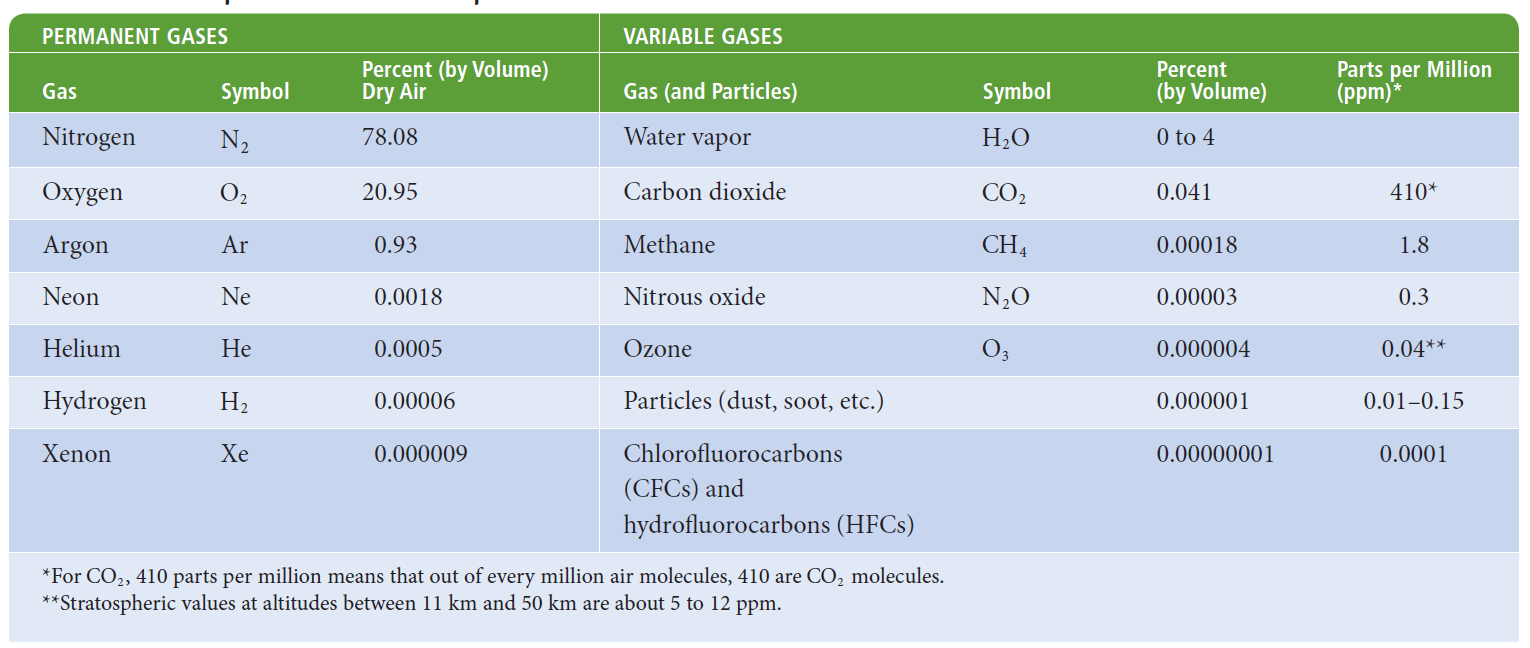
\includegraphics[width=0.8\linewidth]{figures/Table11} \end{center}
\end{center}

\begin{figure}

{\centering 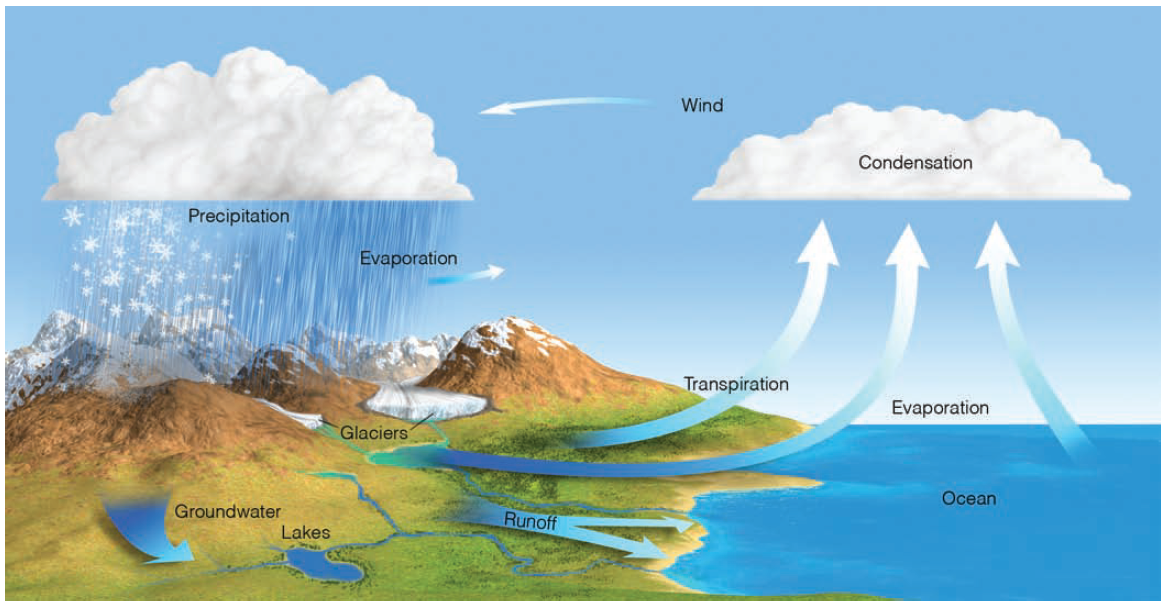
\includegraphics[width=0.8\linewidth]{figures/Figure11} 

}

\caption{XX}\label{fig:intro}
\end{figure}

\textbf{Aerosols} are all tiny solid and liquid suspended particles in
the atmosphere which play a very important role as condensation nuclei
for cloud formation but also have an impact on radiation balance. They
can originate from anthropogenic (e.g.~industry) sources and natural
sources (e.g.~volcanic eruptions). They cause the so-called global
dimming effect. Generally, they are present in low concentrations but
these concentrations vary strongly in space and time depending on
different individual events or trends such as volcanic eruptions or
industrial activities (the latter is cause cleaner air in Europe and
more aerosols over China over the past decade).

\subsection{The atmosphere's layers}\label{the-atmospheres-layers}

Because of gravity almost all air particles are in the first km above
the earth surface. The air becomes very thin very fast. The \textbf{air
density} will decrease exponentially with height. The \textbf{air
pressure} will decrease exponentially because air pressure is the weight
of the air above it. If you are on top of the mount Everest (5.5 km
high) you are above 50\% of the air molecules. In this way we can look
at the atmosphere vertically.

\begin{figure}

{\centering 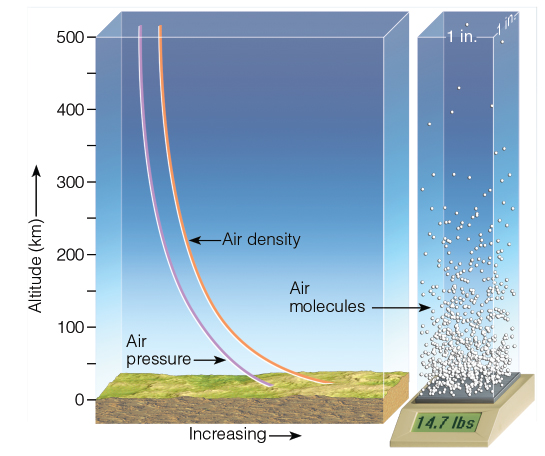
\includegraphics[width=0.4\linewidth]{figures/Figure12a} 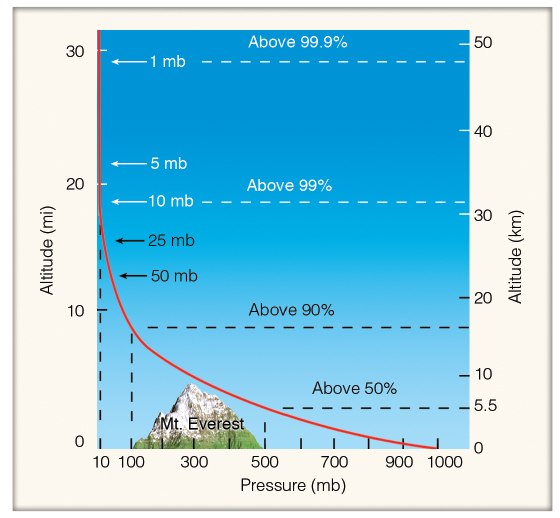
\includegraphics[width=0.4\linewidth]{figures/Figure12b} 

}

\caption{Caption}\label{fig:Layers}
\end{figure}

However, in meteorology we mostly look at \textbf{the vertical
temperature profile}. Based on this profile the atmosphere is divided in
layers. One of the only ways to measure a vertical temperature profile
is to use a radiosonde (i.e.~weather balloon). Typically, the
temperature declines when the balloon goes higher till it reaches -50°C
at an altitude of around 10 km (airplanes fly at this height). The
temperature declines in this first layer (the \textbf{troposphere})
because the sun heats the surface, so the further from the surface the
colder it gets. The altitude where the temperature eventually stops
decreasing is called the \textbf{tropopause}. Above the tropopause there
is a \textbf{permanent temperature inversion} where the temperature will
increase with height, which is called the \textbf{stratosphere}. The
inversion is caused by the ozone layer, where ozone captures
UV-radiation of the sun, heating up the layer from the top to the
bottom. The stratosphere is a very stable layer with cold air the bottom
and warm air at the top (no turbulence, no transfer between layers --
lid on the troposphere, see chapter on atmospheric stability).
Troposphere is most important for us because this is where the weather
is. Everything we will discuss in this course are variations in the
troposphere. You don't have any cloud formation above the tropopause.
The stratosphere/inversion reaches till 50 km high where there is again
a stabilisation and the temperature will decrease with the height again
(\textbf{mesosphere}). Eventually we reach the \textbf{thermosphere}
where the temperature increases very quickly because molecules will
react very strongly with incoming solar radiation, and solar winds.
Dependent on the solar activity the temperature curve will look
differently (there is no buffer effect from the stratosphere here).

\begin{figure}

{\centering 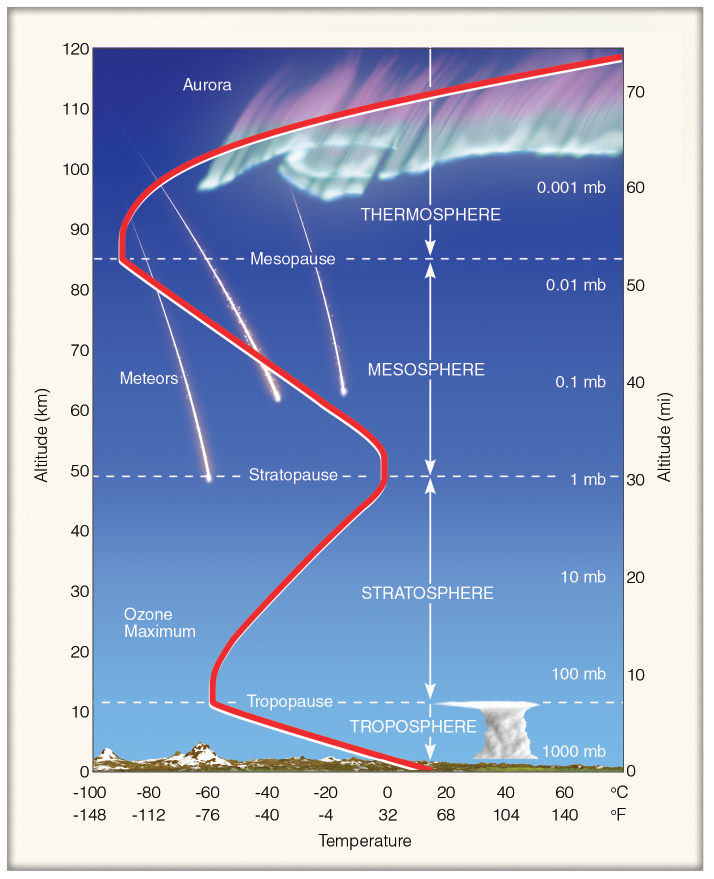
\includegraphics[width=0.8\linewidth]{figures/Figure13} 

}

\caption{Caption}\label{fig:Layer2}
\end{figure}

\textbf{Homosphere} is the lower part of the atmosphere where the
chemical composition is very constant (except ozone in ozone layer)
while in the \textbf{heterosphere} is very variable because of the
interaction with solar radiation.

\begin{figure}

{\centering 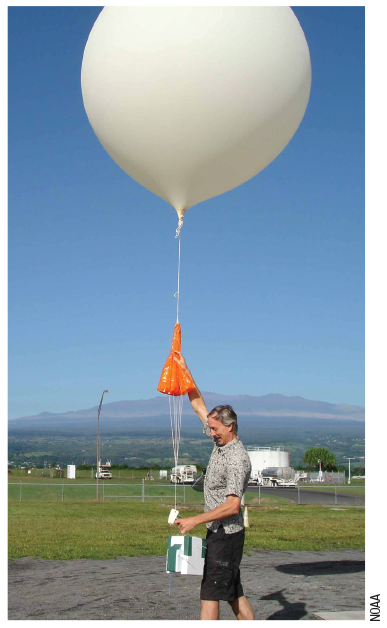
\includegraphics[width=0.4\linewidth]{figures/Figure14a} 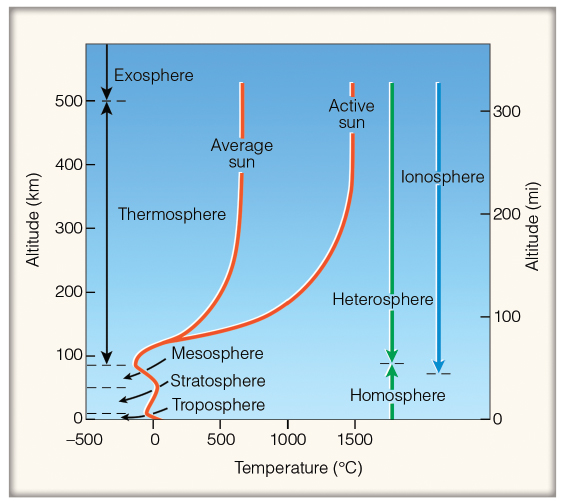
\includegraphics[width=0.4\linewidth]{figures/Figure14b} 

}

\caption{Caption}\label{fig:Homosphere}
\end{figure}

10 km is the average \textbf{thickness of the troposphere}. Because of
the earth rotation the height of the tropopause is highest at the
equator (18 km) and lowest at the poles. This thickness also varies with
the seasons, in the summer (in the NH) there is an expansion of the
lower layer because there is more warming of the earth surface.
Therefore, the highest clouds found in Belgium are at around 10 km high
while in the tropics this will be almost double the height (till 18 km
high) and at the poles only 6 or 7 km high.

\begin{figure}

{\centering 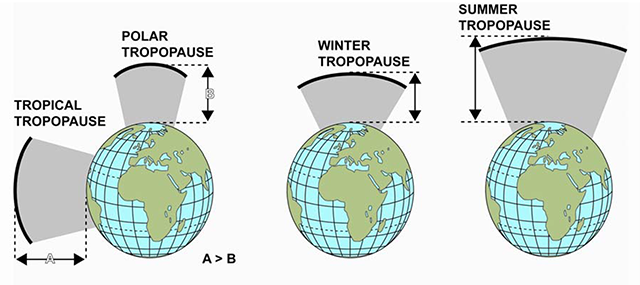
\includegraphics[width=0.5\linewidth]{figures/Figure15} 

}

\caption{Caption}\label{fig:Thickness}
\end{figure}

\section{Meteorology and
ecoclimatology}\label{meteorology-and-ecoclimatology}

\subsection{Difference bteween weather and
climate}\label{difference-bteween-weather-and-climate}

What is the difference between weather \& climate? Both terms are
pointing at the condition of the atmosphere, the difference lies in the
temporal perspective. \textbf{Weather} is about the short term, the
variation in the atmosphere from day to day, within days.
\textbf{Climate} is average weather (e.g. ``what is the average
temperature in September in Belgium'', ``How will this climate vary from
month to month, over the years''). Climate change is a directional
change of the average weather (e.g. ``Is our climate becoming on average
warmer?'') within timescales of decades, centuries.

If the figure below presents the probability function of temperature (or
wind speed or air humidity), then in meteorology we want to know where
we are on this curve next Tuesday for example. We want to predict or
understand why it was 25 °C yesterday and will be 15°C next Tuesday.
Climatology is what is the shape of this curve for our city, where is
the average for our city and how do the tails look for our city. If we
study climate change, then we want to know if the curve will shift, will
the shape change, will the average T be higher in our city, will the
chance to have extreme temperatures change in time? So, there is a
difference in perspective. Weather models want to predict where exactly
we are on this curve, while climate models want to predict how this full
curve will look at the end of the century, and not where we will be on
the curve on the 25 of October 2098.

\begin{figure}

{\centering 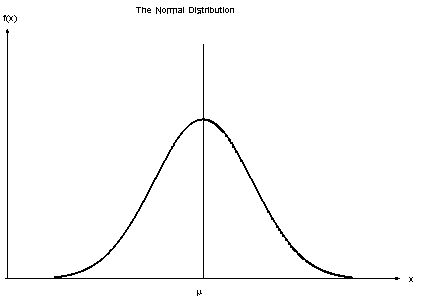
\includegraphics[width=0.4\linewidth]{figures/Figure16a} 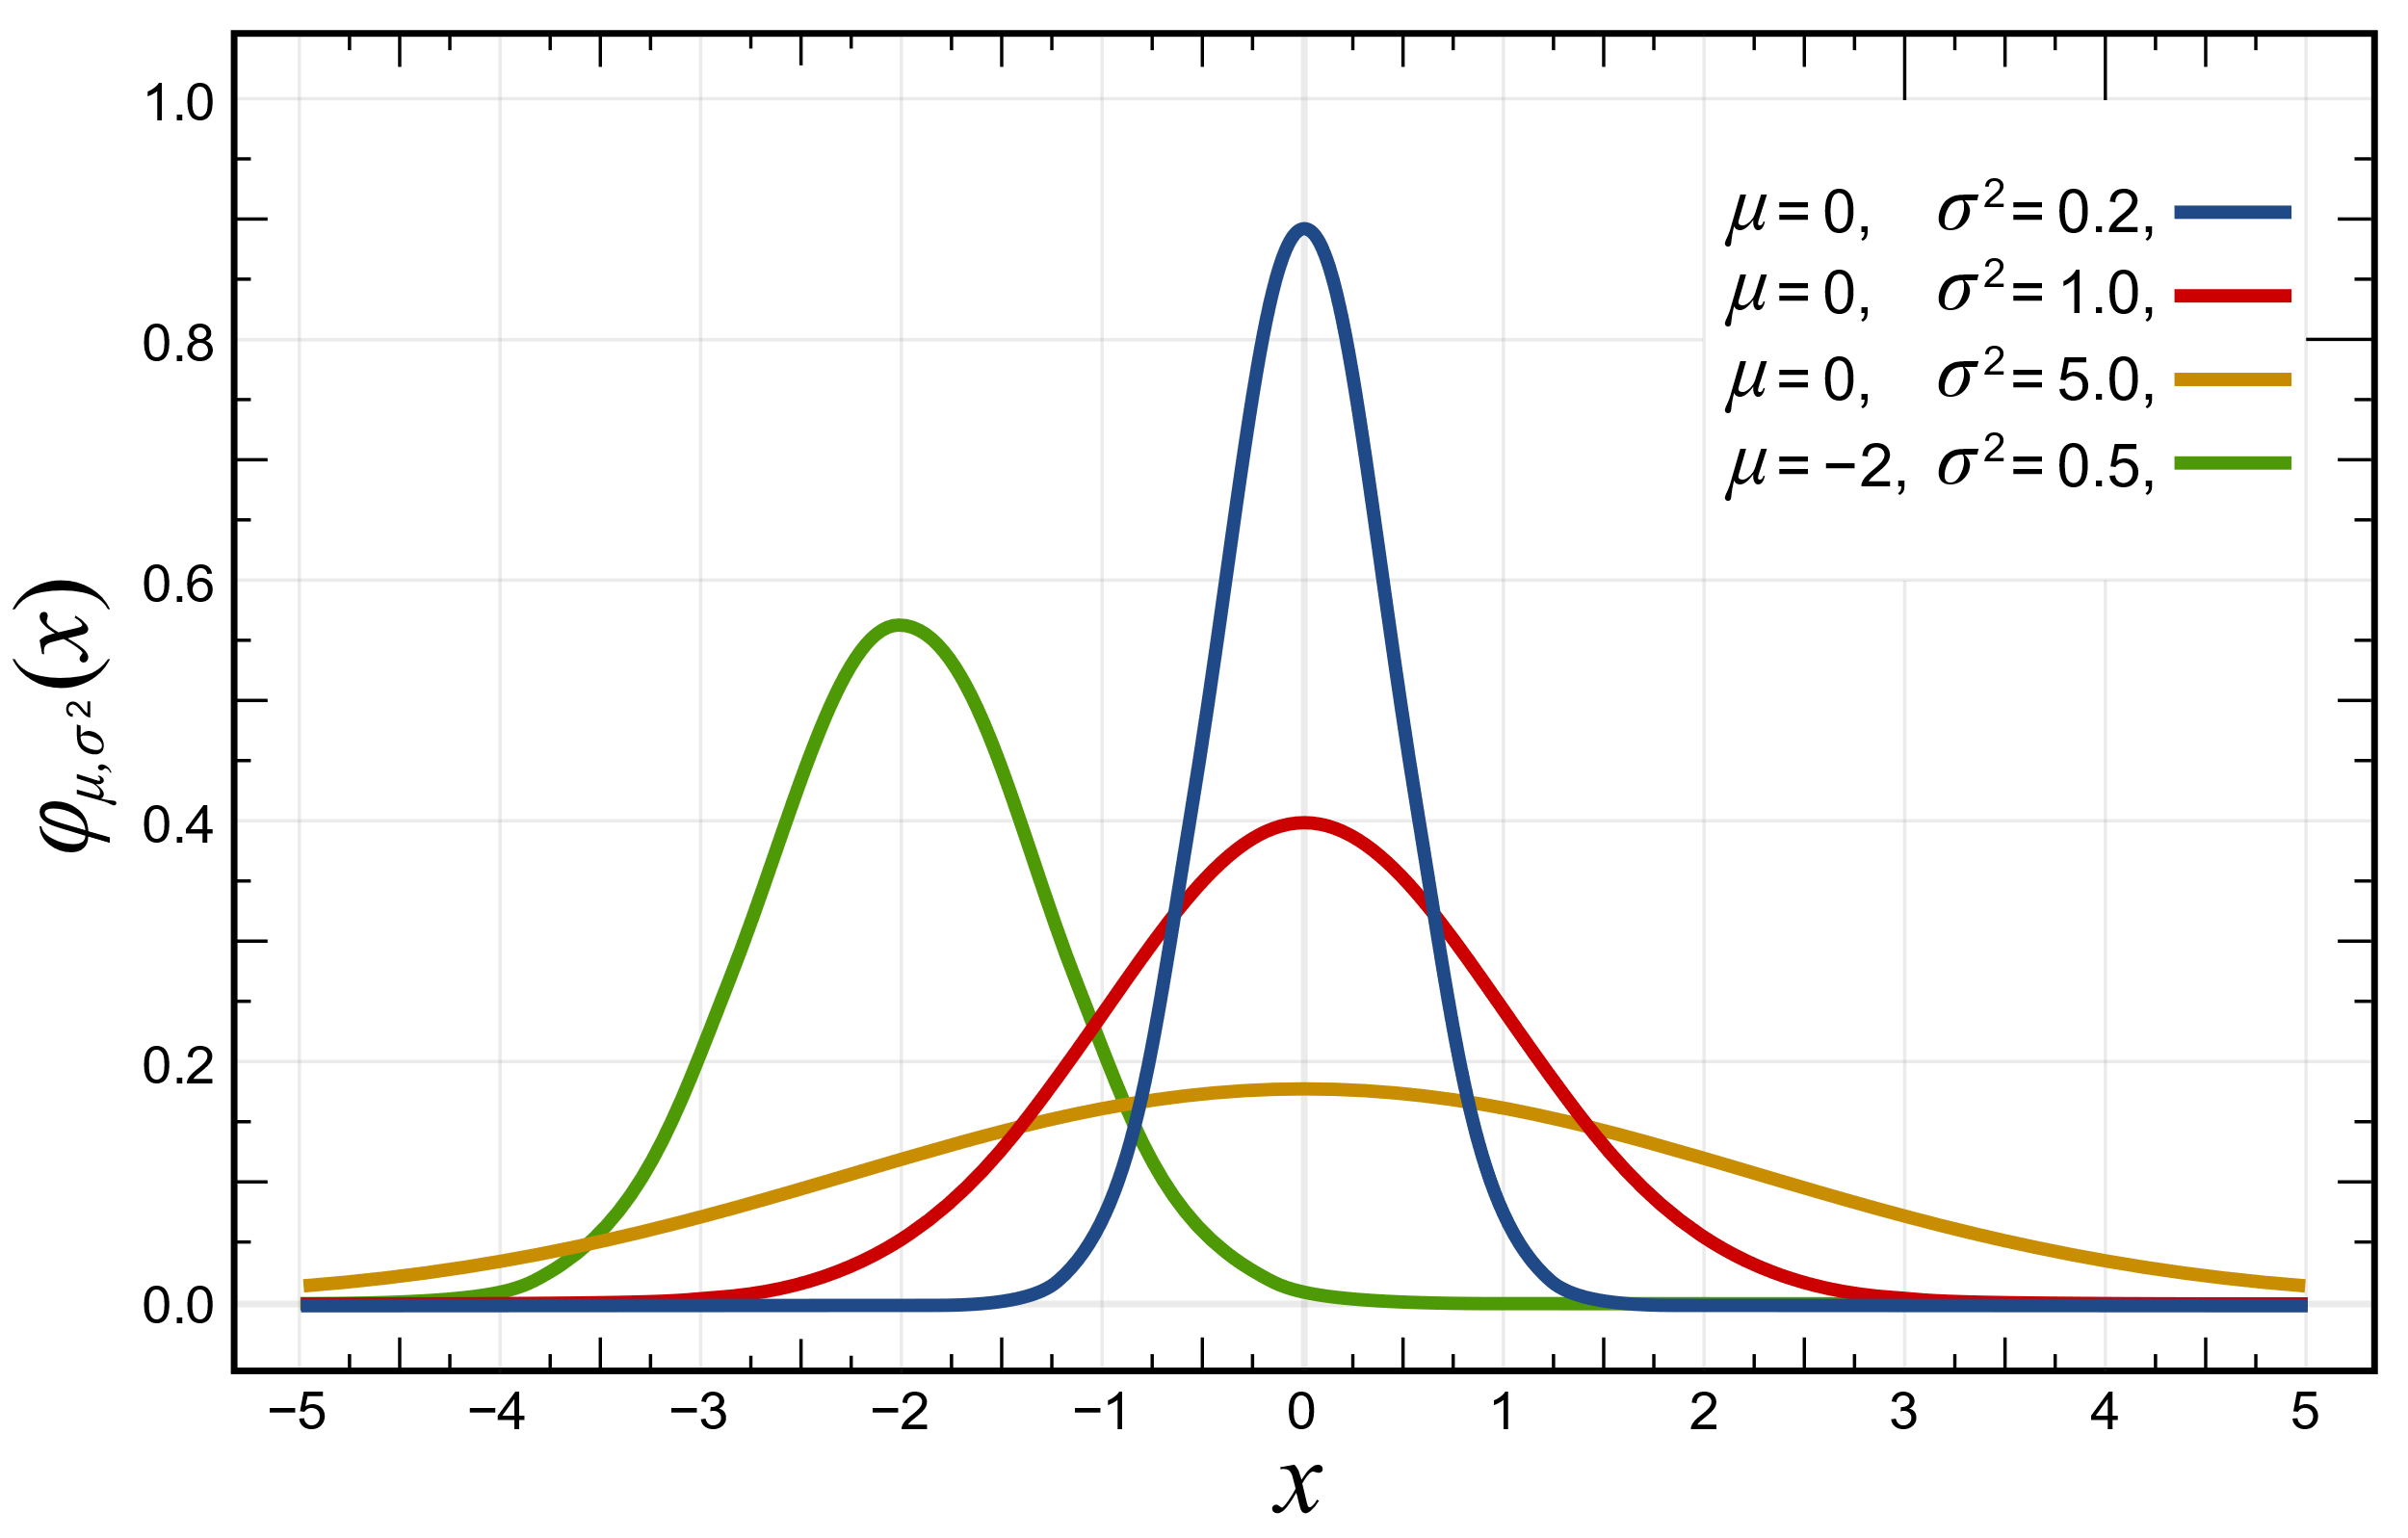
\includegraphics[width=0.4\linewidth]{figures/Figure16b} 

}

\caption{Caption}\label{fig:Climatedef}
\end{figure}

\subsection{History of meteorology}\label{history-of-meteorology}

\textbf{Aristotle} was a philosopher but also the first meteorologist
who wrote a \textbf{descriptive book} (Meteorologica -- ``everything
that happens in the air'') about clouds but also about falling stars and
celestial bodies. The \textbf{next step} happened more than one thousand
years later with the invention of \textbf{measuring equipment}. Galilei
was the first person who made an instrument to measure the temperature,
the thermoscope (bubbles that rise or descend in liquids depending on
the temperature). Several decades later the barometer was invented. This
evolved till we had a set of instruments to measure weather variables
and we could start to continuously measure weather (first observations
in Ukkel in 1833). Then the first \textbf{computers} evolved to super
computers and were used quite rapidly for weather predictions and
climate modelling. After the second world war the first \textbf{radars}
were used for cloud observation and \textbf{weather satellites} were
launched. Today, ground observations are still key and are combined with
remote sensing and simulation models. What we see in weather reports is
based on the combination of these different components (e.g.~weather
stations, remote sensing, climate models). Finality of the part
meteorology in this course is reading and interpreting weather maps that
synthesize al key weather elements.

\begin{figure}

{\centering 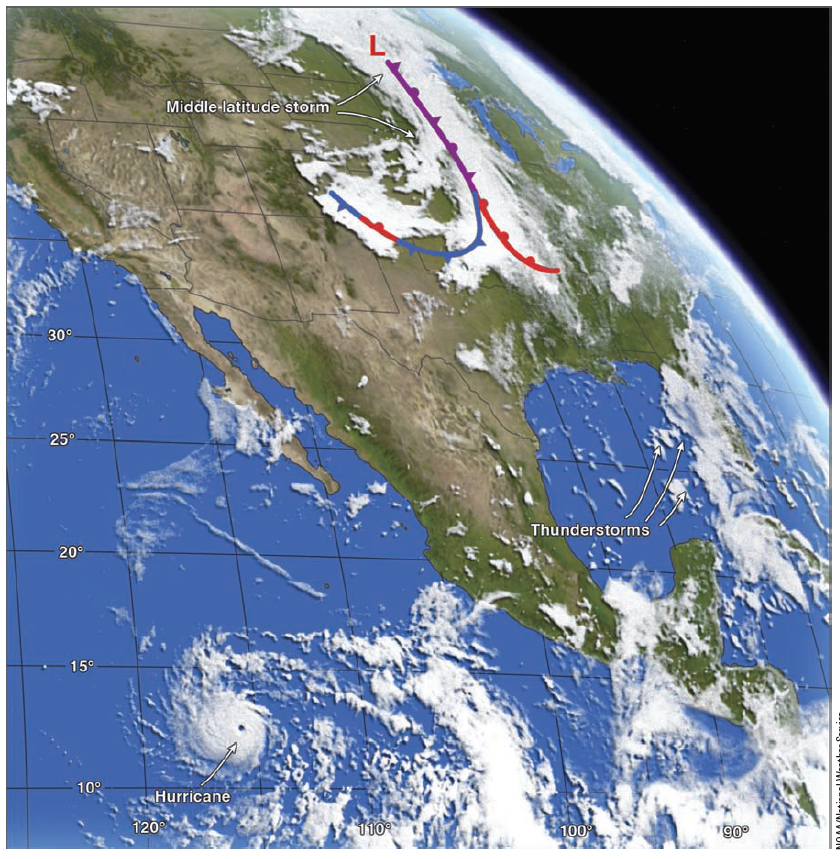
\includegraphics[width=0.5\linewidth]{figures/Figure17} 

}

\caption{Caption}\label{fig:History1}
\end{figure}

\begin{figure}

{\centering 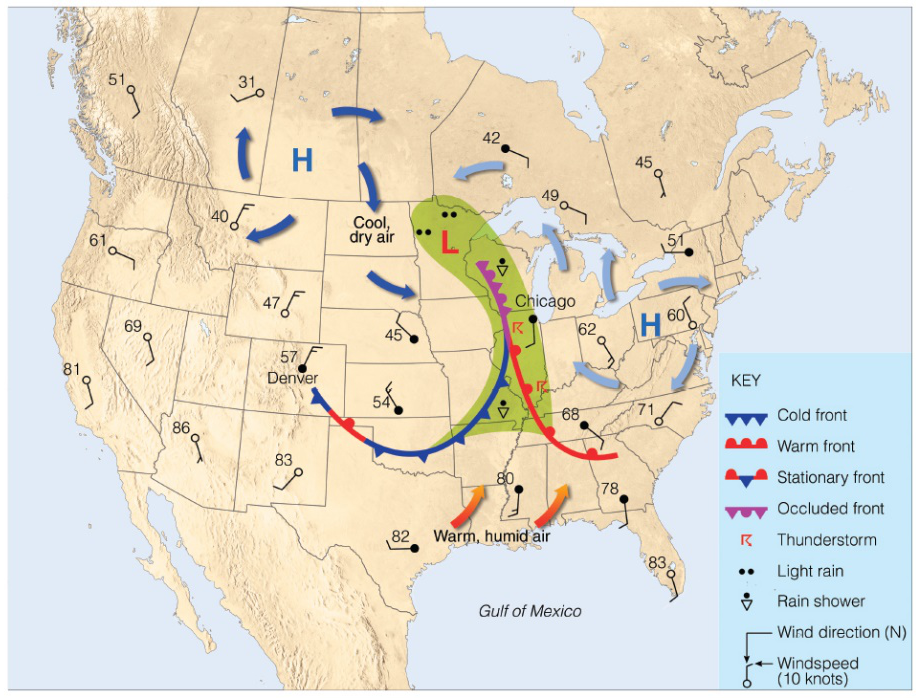
\includegraphics[width=0.5\linewidth]{figures/Figure18} 

}

\caption{Caption}\label{fig:History2}
\end{figure}

\subsection{Weather and climate in our daily
lives}\label{weather-and-climate-in-our-daily-lives}

Weather and climate are very important and determine a lot of aspects in
our lives (e.g.~agriculture, forestry, environmental issues, housing,
economy, clothing) especially extreme events as well as day to day
weather.

\subsection{Ecoclimatology}\label{ecoclimatology}

\textbf{Ecoclimatology} is an interdisciplinary science which links
ecology and climatology. It is about the link between ecosystems and the
climate, between the biosphere and the atmosphere and especially it is
about the interactions. These interactions are determined by fluxes of
energy, water and chemical elements which are exchanged between the
vegetation on the earth surface and the atmosphere.

In the ecoclimatology part of the course, we are going to talk about
biogeography, how does the climate determine which vegetation occurs on
certain places on the planet, but also about the impact of climate
variations on crops, plants, natural ecosystems and what are the
feedbacks (how do ecosystems affect the climate in their term). We will
also discuss and use vegetation models, which are important tools to
study these interactions.

\subsection{History of Ecoclimatology}\label{history-of-ecoclimatology}

\textbf{Ecoclimatology} is a younger and less developed scientific
branch which started with Theoprasthus (student of Aristotle) who wrote
a descriptive, observational book about plants and where they were
found, linked with weather patterns of that place. In the 1800s (when
measurements were possible), Alexander \textbf{von Humboldt} was the
first one who really made the link between climate and the presence of
certain plants. Later, others continued his work (e.g.~vegetation zones,
Köppen classification) and now there is also a lot of modelling.

\subsection{Biogeoscience}\label{biogeoscience}

\textbf{Biogeoscience} is closely related to ecoclimatology and is
situated on the intersection of the different spheres and studies
interactions between the different spheres. A lot of the current
environmental issues/problems have to be studied within the
biogeosciences, especially when we want to look at the anthropogenic
impact.

\begin{figure}

{\centering 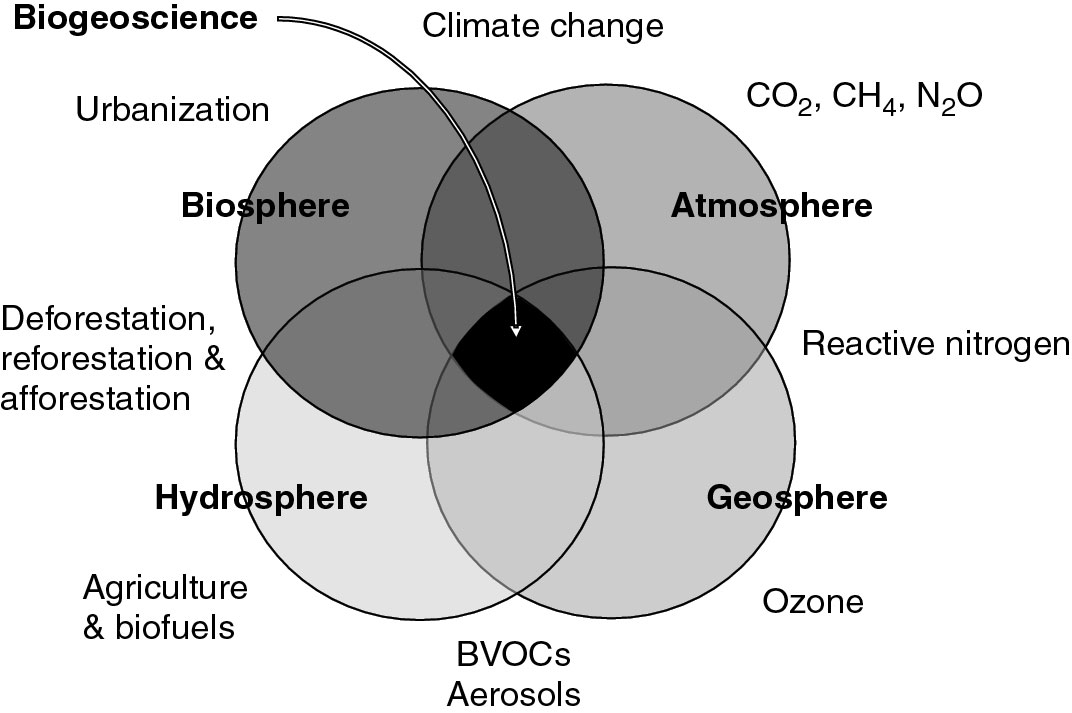
\includegraphics[width=0.5\linewidth]{figures/Figure19} 

}

\caption{Caption}\label{fig:Biogeoscience}
\end{figure}

\begin{figure}

{\centering 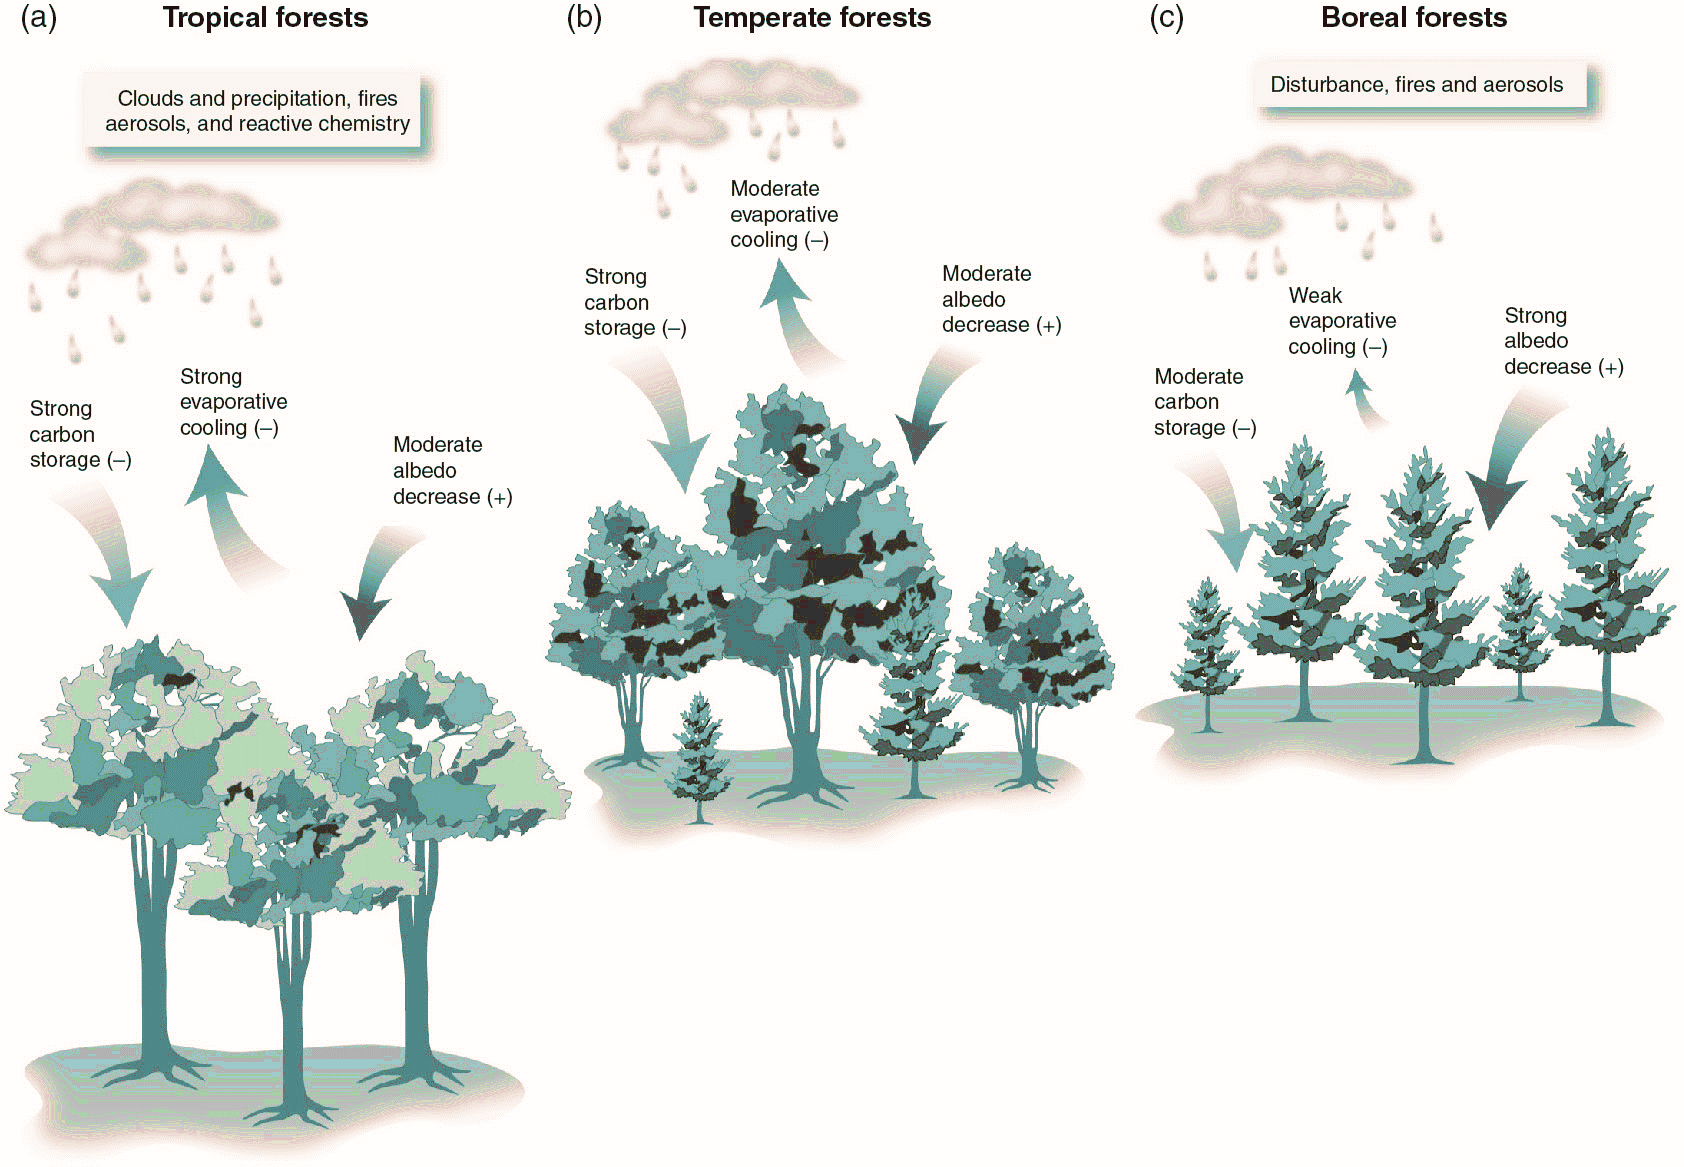
\includegraphics[width=0.8\linewidth]{figures/Figure110} 

}

\caption{Caption}\label{fig:Biogeoscience2}
\end{figure}

A good example of the role of vegetation in land-atmopshere interactions
is the given by forests. Forest provide ecosystem services, but these
are dependent on the type of forest (e.g.~a tropical rainforest versus a
boreal forest will affect the climate in different ways). For example,
the impact on the albedo (reflectivity earth surface) will be greater
when a boreal forest grows than the contribution of a tropical forest.
In the contrary, the evaporation and carbon storage of one hectare of
tropical forest will be greater than one hectare of boreal forest ((-)
cooling effect (+) warming effect).

\subsection{Key land-atmosphere
interactions}\label{key-land-atmosphere-interactions}

Interaction between land and climate has an influence on a lot of
biophysical processes. The reflectivity (\textbf{albedo}) of the earth
surface will influence the energy balance. The \textbf{roughness} of the
earth surface is determined by the type of vegetation, causing different
wind patterns and turbulence, which in its turn impacts the \textbf{heat
and gas exchange}. The physiology of the stomata of plants will have an
influence on \textbf{water exchange}. Soil moisture will also have an
impact. The \textbf{carbon cycle} has an impact on the CO2 in the
atmosphere and will depend on the type of vegetation. \textbf{Nitrogen
exchange} (N-deposition from industry or N2O as greenhouse gas from
soils) will be different in an agricultural area compared to a forest.
\textbf{Aerosols} will determine the solar radiation a forest gets which
has an impact on photosynthesis and the carbon balance. Forests will
also emit \textbf{volatile organic carbons} (e.g.~isoprene a lot in
tropical forests) which are precursors of aerosols, so forests have an
impact on the amount of aerosols in the atmosphere (also when a forest
burns this brings a lot of particles in the air). Ecoclimatology studies
many of these elements.

\begin{figure}

{\centering \includegraphics[width=0.8\linewidth]{figures/Figure112} 

}

\caption{Caption}\label{fig:Land}
\end{figure}

\begin{figure}

{\centering \includegraphics[width=0.8\linewidth]{figures/Figure113} 

}

\caption{Caption}\label{fig:Land2}
\end{figure}

\section{Energy, temperature and
heat}\label{energy-temperature-and-heat}

\subsection{Definitions}\label{definitions}

\textbf{Energy} is defined as the capacity to do work. Potential
(static) and kinetic energy (dynamic) are types of energy. Energy can
take on different forms. \textbf{Temperature} is a measure for kinetic
energy (e.g.~air temperature is the kinetic energy of the air molecules
in our atmosphere). Therefore, making an energy balance is essential to
understand the climate. \textbf{Heat} is the exchange, transfer of
energy from one medium to another, it is a flux of energy.

\subsection{Temperature}\label{temperature}

Temperature is a \textbf{measure for kinetic energy} (e.g.~how much will
the molecules collide with each other and against the edges of the
volume it is confined in). Temperature is measured in ° Celsius,
Fahrenheit, Kelvin (most scientific scale). The average temperature on
earth is typically 15 °C, but weather stations typically measure
variations between -30 °C up to 40 °C.

\begin{figure}

{\centering 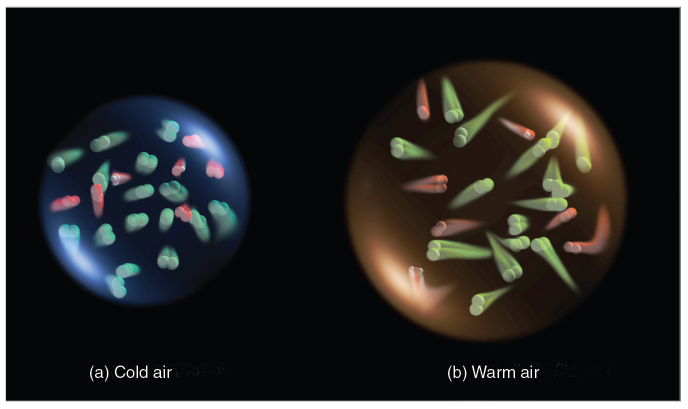
\includegraphics[width=0.5\linewidth]{figures/Figure114} 

}

\caption{Caption}\label{fig:Temperature}
\end{figure}

\begin{figure}

{\centering 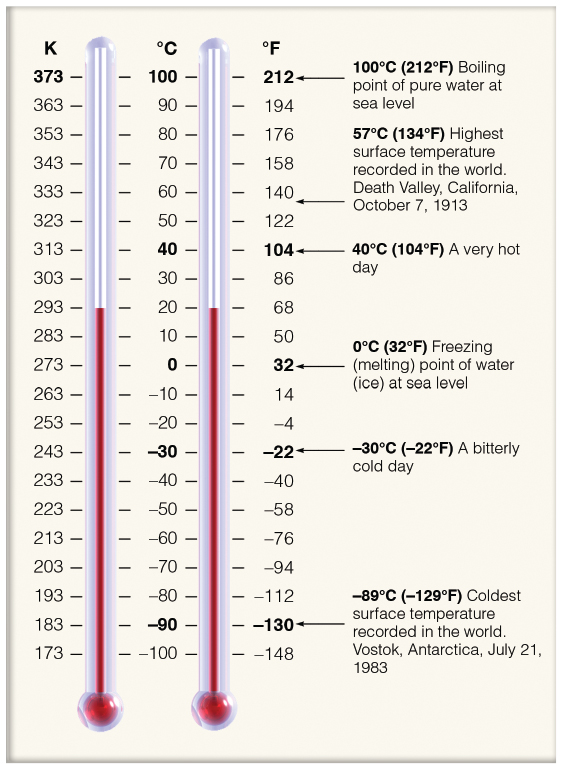
\includegraphics[width=0.5\linewidth]{figures/Figure115} 

}

\caption{Caption}\label{fig:Temperature2}
\end{figure}

\subsection{Specific heat}\label{specific-heat}

Different media which exist in natural systems can have very different
specific heats expressed as J per kg per °C, it is the amount of energy
needed to increase the temperature of 1 kg of a substance with 1 °C
(e.g.~a rock or sand will heat up faster than ice or wet soil -- see
table x). Water needs a very high amount of energy to heat up 1 °C (you
need four times more energy to heat up a kg of water than a kg of air).
Ice needs less energy than liquid water which is important for the
climate system (e.g.~oceans heat up slower than land and humid areas
have a large buffering capacity). This is also why there is so much heat
transfer involved with evaporation and condensation of water (latent
heat).

\begin{center}
\captionof{table}{Specific heat of various substances}
\label{table:Sheat}

\begin{center}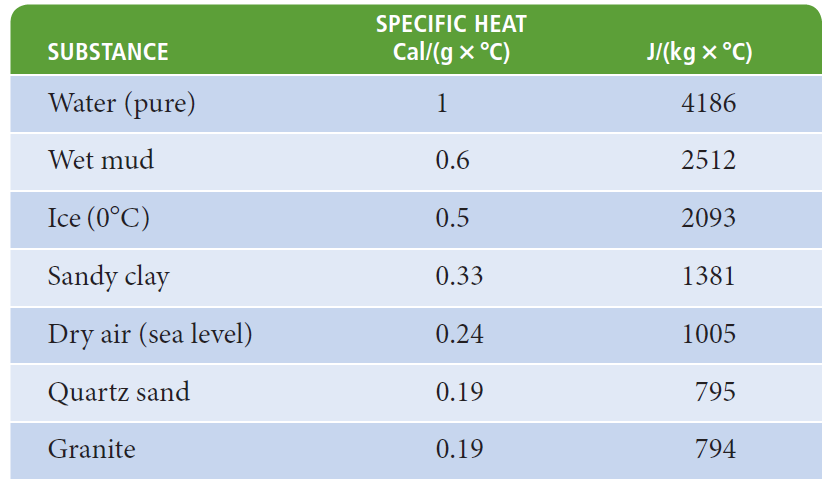
\includegraphics[width=0.8\linewidth]{figures/Table12} \end{center}
\end{center}

\subsection{Latent and sensible heat}\label{latent-and-sensible-heat}

\textbf{Sensible heat} is the energy used to change the temperature of
the air. Sensible heat flux can be measured by a temperature change.
\textbf{Latent heat} is the energy used to change the phase of a
substance while the temperature does not change (e.g.~energy needed to
evaporate water or melt ice). \textbf{Evaporation is a cooling process}
for the environment because the substance takes up heat from the
environment to evaporate while \textbf{condensation is a warming
process} for the environment because the process releases heat to the
environment. Important to understand these concepts to understand the
climate system (e.g.~when a cloud forms water vapor will condensate to
form water droplets which is accompanied by a release of energy to the
environment.)

\begin{figure}

{\centering 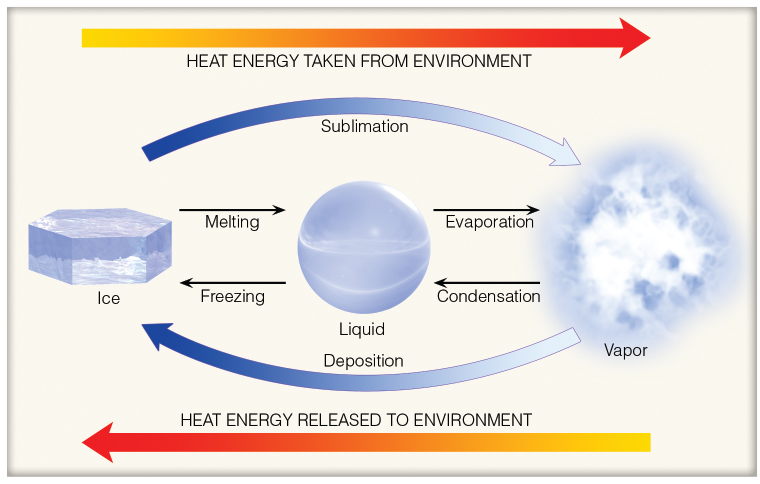
\includegraphics[width=0.7\linewidth]{figures/Figure116} 

}

\caption{Caption}\label{fig:LSheat}
\end{figure}

\subsection{Heat transfer in the
atmosphere}\label{heat-transfer-in-the-atmosphere}

There are three ways in which heat is transferred in the atmosphere:
\textbf{convection, conduction and radiation}. Radiation is based on
radiation from the sun or other objects (every object with a temperature
higher than 0 K emits radiation). Radiation does not heat the medium,
air (imagine feeling the radiative heat of the sun on your skin on a
cold winter day). Convection is the transfer heat via a fluid which is
typically air in meteorology (hot air bubbles which are moving to
transfer energy in the atmosphere). Convection does heat the medium.
Conduction is heat transfer through a solid substance. This can be
neglected in meteorology because air has a really low heat conductivity.
There is only a small amount of heat that is transferred via conduction
from the soil to the first layers of air above it. The largest heat
fluxes on earth are governed by radiation and convection.

\begin{figure}

{\centering 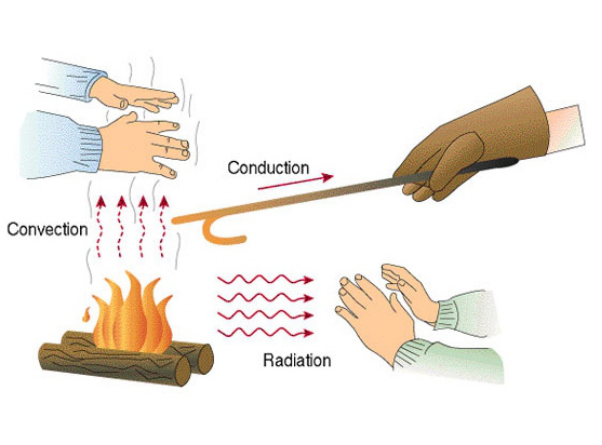
\includegraphics[width=0.5\linewidth]{figures/Figure117} 

}

\caption{Caption}\label{fig:Heattransfer}
\end{figure}

\begin{figure}

{\centering 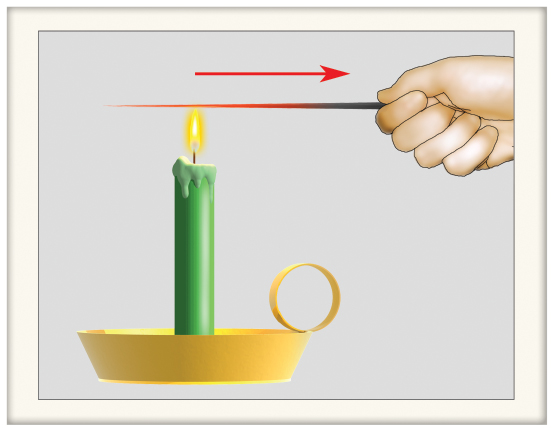
\includegraphics[width=0.5\linewidth]{figures/Figure118} 

}

\caption{Caption}\label{fig:Heattransfer2}
\end{figure}

\textbf{Convection} happens when the sun heats a specific spot on the
earth (for example a dark plowed field that heats up more than the
grassland surrounding it), the air above this hot surface heats up and
this hot air bubble rises and moves in the atmosphere
(\textbf{thermal}). A lot of the energy transfer on earth happens
through these thermals, through convection. This is not the same as
\textbf{advection} which is the horizontal transfer of any property,
this can be energy a gas or pollutants (e.g.~cold air or pollutant
sliding of a mountain) while convection is the three dimensional
transfer of heat through hot air bubbles.

\begin{figure}

{\centering 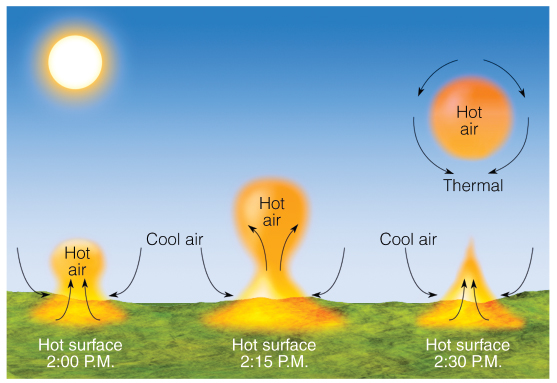
\includegraphics[width=0.7\linewidth]{figures/Figure119} 

}

\caption{Caption}\label{fig:Heattransfer3}
\end{figure}

\section{Radiation}\label{radiation}

Radiation is electromagnetic waves which don't heat the medium (air).
Direct sun rays lose almost no energy before reaching earth. The
\textbf{wavelength} of radiation determines its energy. A quantum of
light with a high frequency (short wavelength) has more energy than one
with a high wavelength.

\begin{figure}

{\centering 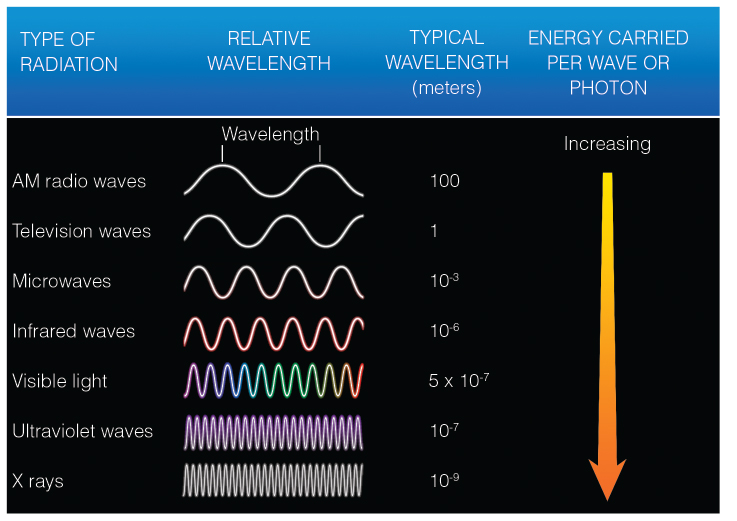
\includegraphics[width=0.8\linewidth]{figures/Figure120} 

}

\caption{Caption}\label{fig:Radiation}
\end{figure}

\subsection{Important laws}\label{important-laws}

A first important law describes the energy of a photon (ep) with a
certain wavelength (lambda):

\begin{equation} 
  e_p = h  \frac{c}{\Lambda}
  \label{eq:Eq1}
\end{equation}

h = 6.626 x 10-34 J s (planck's constant) c = 3 x 108 m s-1 (speed of
light)

Secondly, \textbf{Planck's law} relates the radiant flux density per
unit wavelength emitted by a black body (W m-2 m-1) to the wavelength
(lambda) and temperature (T) (e.g.~spectrum of the sun when you fill in
T of the sun):

\begin{equation} 
  E(\Lambda) =\frac{2 \pi h c^2}{\Lambda^5\left(exp(hc/k\Lambda T) - 1 \right)}
  \label{eq:Eq2}
\end{equation}

Thirdly, \textbf{Wien's displacement law} relates the wavelength of
maximum emission to the temperature of a black body:

\begin{equation} 
  \Lambda_{max} = 2897 \mu m K / T 
  \label{eq:Eq3}
\end{equation}

Lastly, the \textbf{Stefan-Boltzmann law} relates the radiant flux
density emitted by an object (E) to its temperature obtained by
integrating over all wavelengths:

\begin{equation} 
  E = \epsilon \sigma T^4
  \label{eq:Eq4}
\end{equation}

E = Emittance \(W \cdot m^{-2}\)\\
\(\sigma\) = 5.67 x \(10^{–8}\) \(W \cdot m^{–2} \cdot K^{–4}\)
(Stefan--Boltzmann constant)\\
\(\epsilon\) (broadband emissivity)

These laws are summarized in the figure which gives the spectrum of
emitted energy for the sun and the earth (unit:
\(W \cdot m^{-2} \cdot µm^{-1}\) -- the energy intensity per spectral
band spectral intesity). The curve is determined by the temperature of
the sun (6000 K) and earth (288 K) (Planck's law). The colder the object
the longer the wavelength at which this maximum energy intensity is
reached (Wien's law). The amount of total radiation is given by the
surface under the curve (Stefan-Boltzmann law). The sun emits
\textbf{shortwave} radiation (\(\lambda_{max}\) at 0.5 µm) while the
earth emits \textbf{longwave} (invisible) radiation (lambda max at 10
µm) (both short and longwave radiation are important radiation
components). Thus, the sun emits compared to the earth, radiation of a
different quality and quantity.

\begin{figure}

{\centering 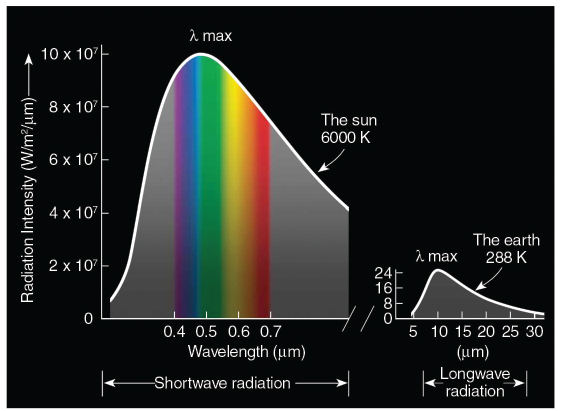
\includegraphics[width=0.5\linewidth]{figures/Figure121} 

}

\caption{Caption}\label{fig:Laws}
\end{figure}

\subsection{The sun's EM spectrum}\label{the-suns-em-spectrum}

This figure shows the percentages of solar-energy in the different
wavelength bands. Almost everything is infrared (37+11) and visible
light (44). Only a few percentages are UV light, however, containing a
lot of energy (ozon layer protects us from this). This is the spectrum
that reaches the earth before entering the atmosphere.

\begin{figure}

{\centering 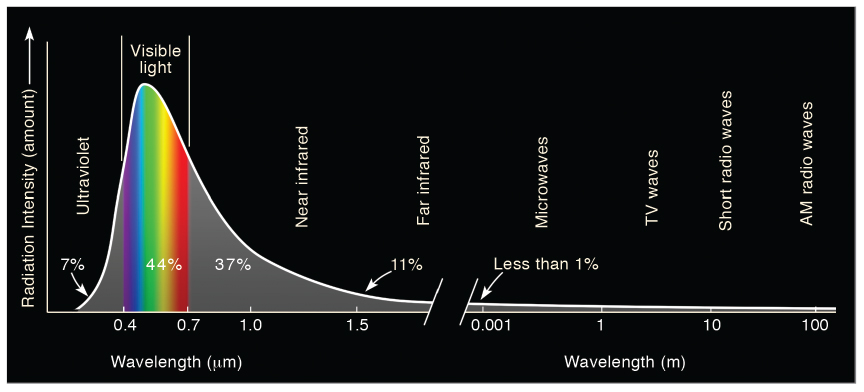
\includegraphics[width=1\linewidth]{figures/Figure122} 

}

\caption{Caption}\label{fig:Spectrum}
\end{figure}

\subsection{Absorption, reflection and
transmission}\label{absorption-reflection-and-transmission}

Once the radiation enters the atmosphere, there is a lot of interaction
of the radiation with the molecules in the atmosphere and the earth
surface (this changes the nice curve from before). The radiation can be
reflected, absorbed or transmitted (e.g.~light transmitted through the
leaves of a tree).

\begin{figure}

{\centering 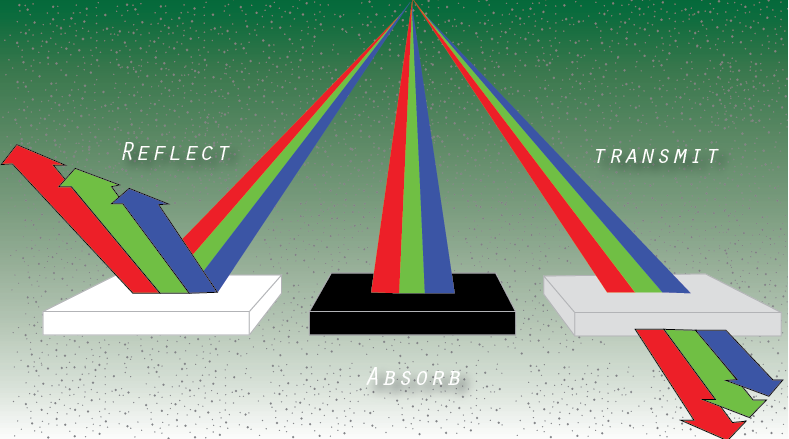
\includegraphics[width=0.5\linewidth]{figures/Figure123} 

}

\caption{Caption}\label{fig:Spectrum2}
\end{figure}

\subsection{Scattering}\label{scattering}

Scattering happens when the sun rays collide with molecules and are
reflected resulting in diffuse radiation. There are two mayor ways of
diffusion. Firstly, \textbf{Rayleigh scattering} is the scattering of
light by gas molecules which have a smaller diameter than the wavelength
of the light. This is a continous form of scattering of which the
intensity is inversely proportional to the wavelength (
\textasciitilde{} \(\lambda^{-4}\)). So, short wave lengths (high
energy) will be scattered more than long wavelengths. This is the reason
blue light is scattered more and the sky looks white at noon looking
straight at the sun, blue when not looking straight at it and red in the
evening (looking straight at the sun) as all the blue light is already
scattered away. Secondly there is \textbf{Mie scattering}, which is the
scattering of light by molecules with a diameter larger than the
wavelength of the light (e.g.~aerosols, water droplets in clouds, ice,
smoke). For Mie scattering, the intensity is not proportional to the
wavelength, every wavelength is scattered equally in all directions
(this is why clouds look white or grey).

\begin{figure}

{\centering 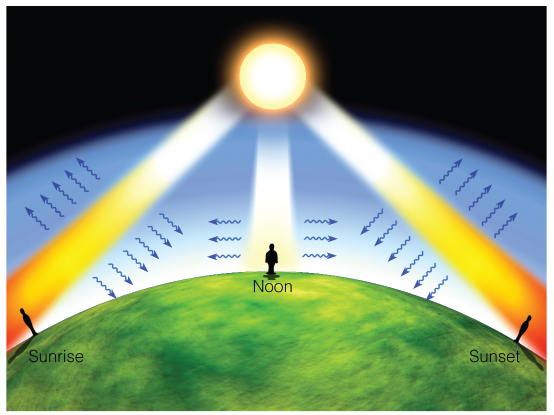
\includegraphics[width=0.5\linewidth]{figures/Figure124} 

}

\caption{Caption}\label{fig:Scattering}
\end{figure}

\begin{figure}

{\centering 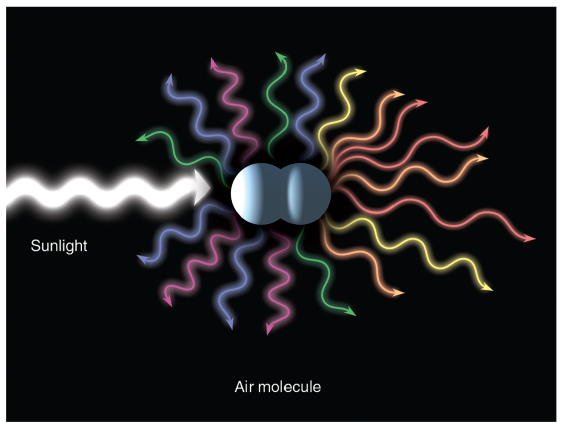
\includegraphics[width=0.5\linewidth]{figures/Figure125} 

}

\caption{Caption}\label{fig:Scattering2}
\end{figure}

\begin{figure}

{\centering 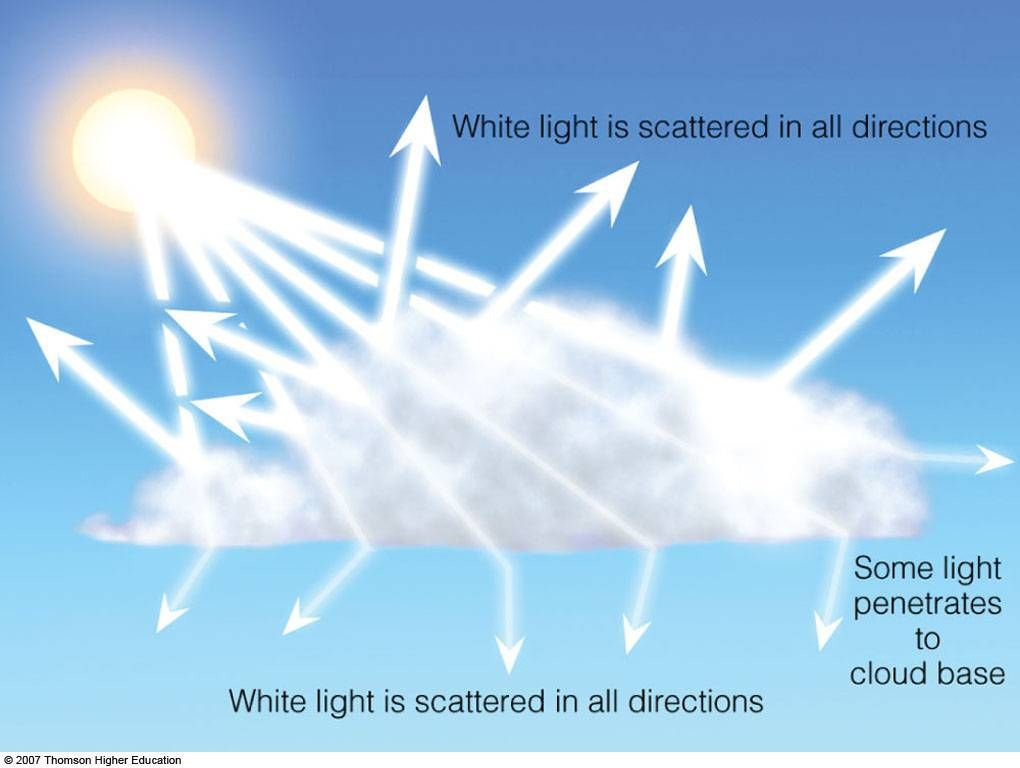
\includegraphics[width=0.5\linewidth]{figures/Figure126} 

}

\caption{Caption}\label{fig:Scattering3}
\end{figure}

\subsection{Direct and diffuse
radiation}\label{direct-and-diffuse-radiation}

The \textbf{shortwave direct} (Sh) and \textbf{diffuse} (Sd)
\textbf{radiation} coming from the sun are measured with a
\textbf{pyranometer}. This sensor measures the total shortwave radiation
(St=Sh+Sd) in watts per square meter, so the radiation measured is also
dependent on the solar angle (low angles, greater spread over the
surface). When using a pyranometer which tracks the solar activity and
always measures the direct shortwave radiation perpendicular (Sb), we
correct for the solar elevation (β): Sh=Sb x sinβ. On average we would
measure 740 Watt/m2 at noon on a sunny day in Belgium.

\begin{figure}

{\centering 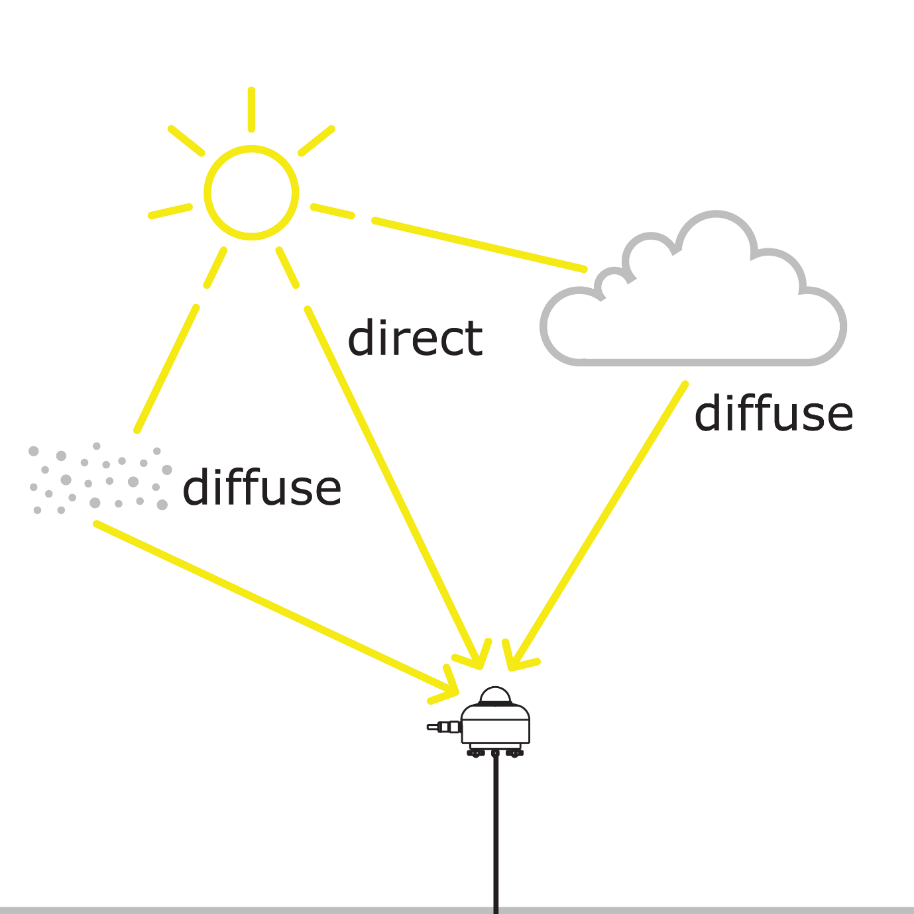
\includegraphics[width=0.5\linewidth]{figures/Figure127} 

}

\caption{Caption}\label{fig:Diffuse}
\end{figure}

This figure shows the shortwave radiation coming from the sun measured
at the earth surface (during a cloudy day). Compared to the radiation
measured at the top of the atmosphere certain wavelengths have vanished.
These wavelengths were absorbed by molecules in the air. The energy
quantity coming from diffuse radiation is typically less than the energy
coming from direct radiation. The quality is also different, the peak in
diffuse radiation can be found in the shorter wavelengths (blue light).
Plants can efficiently use these wavelengths present in diffuse
radiation.

\begin{figure}

{\centering 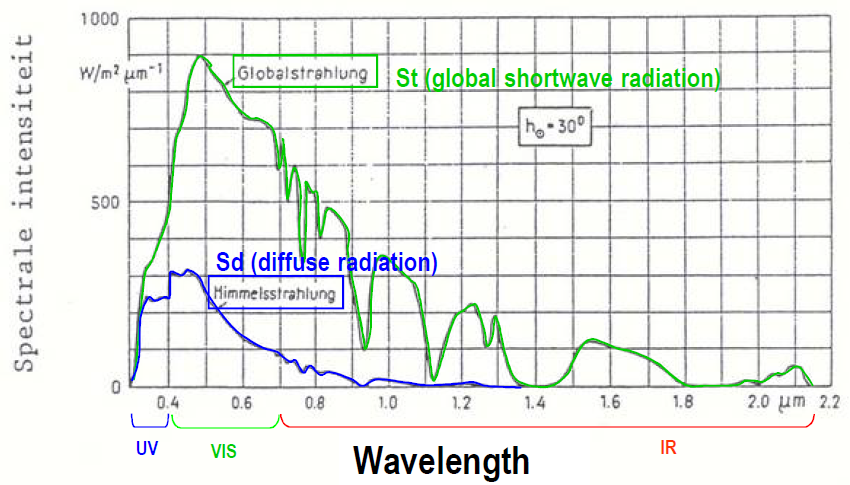
\includegraphics[width=0.9\linewidth]{figures/Figure128} 

}

\caption{Caption}\label{fig:Diffuse2}
\end{figure}

These figures present the sensitivity of the human eye and the
sensitivity of plants to light. Plants typically absorb (pigments in the
leaf) blue and red light and less green light which is why they look
green. This total spectrum is slightly different than the spectrum which
the human eye is sensitive to but it spans the same wavelengths (400 nm
-700 nm). \textbf{PAR (photosynthetic active radiation)} is the
radiation within these wavelengths which plants can use for
photosynthesis (\(\mu mol \, photons \cdot m^{-2} \cdot s^{-1}\)). This
is approximately half of the incoming shortwave radiation. However, this
also depends on whether the radiation is direct or diffuse and the solar
elevation. In diffuse radiation there is relatively more PAR radiation
and at lower solar elevations there is relatively less PAR radiation. On
a sunny day there can be 2000 \(µmol \cdot m^{-2} \cdot s^{-1}\) PAR
radiation. The PAR fraction in diffuse and direct light depends on the
solar elevation (Table) at lower solar elevation the path length through
the atmosphere of (especially direct) light is longer, blue light is
scatter out, less PAR remains.

\begin{figure}

{\centering 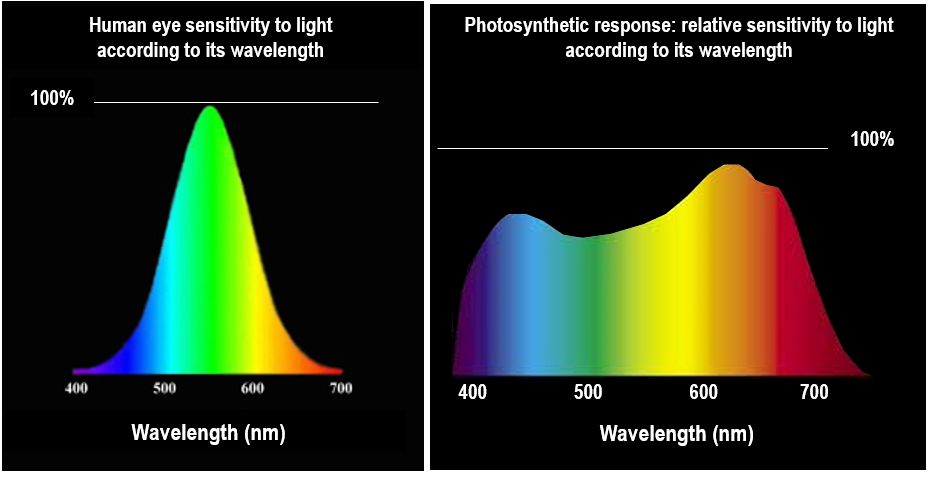
\includegraphics[width=0.8\linewidth]{figures/Figure129} 

}

\caption{Caption}\label{fig:PAR}
\end{figure}

\begin{figure}

{\centering 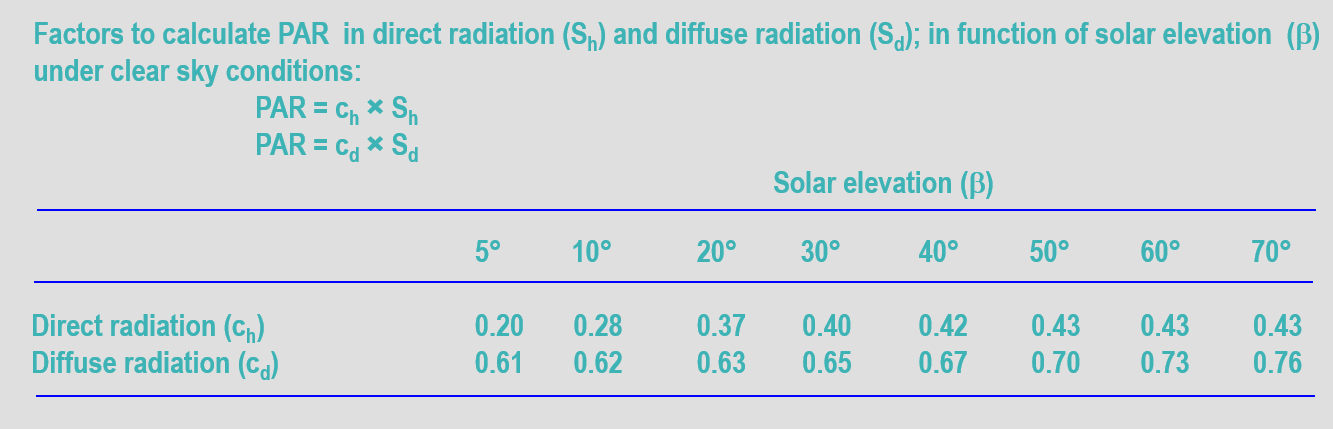
\includegraphics[width=0.9\linewidth]{figures/Figure130} 

}

\caption{Caption}\label{fig:PAR2}
\end{figure}

\subsection{Selective
absorbers/emitters}\label{selective-absorbersemitters}

The spectrum of light that we receive at the surface of the earth looks
different than the spectrum received at the top of the atmosphere
because of selective absorbers. This figure shows the different
\textbf{absorption spectra} for different gas molecules in the
atmosphere. Ozon mainly absorbs UV light but also infrared light (making
it a greenhouse gas). \textbf{Greenhouse gases} typically absorb
infrared light. CO2, N2O but also water vapor and methane absorb a lot
of infrared radiation. When we look at the total spectrum we see that a
lot of wavelengths are filtered out before they can reach the earth
surface. The visible light does reach the earth surface while UV (short
wavelengths) and a lot of infrared radiation (coming from the sun but
also from the earth) are absorbed. The \textbf{atmospheric window} (a
zone with little absorption) is the group of infrared wavelengths that
can leave the earth surface and the atmosphere again (this is how the
earth loses energy via longwave radiation). However, this atmospheric
window can be closed by clouds which is why a clear night is cooler than
a cloudy night.

\begin{figure}

{\centering 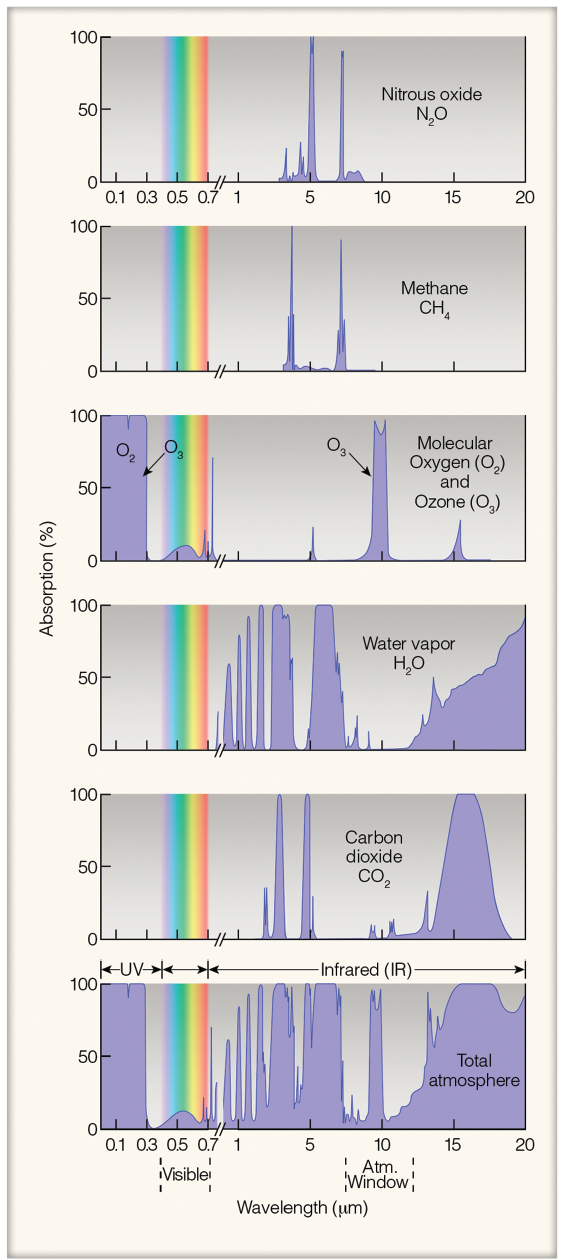
\includegraphics[width=0.5\linewidth]{figures/Figure131} 

}

\caption{Caption}\label{fig:atmwindow}
\end{figure}

\subsection{Greenhouse effect}\label{greenhouse-effect}

When there would be no greenhouse effect (no selective absorbers), the
earth would lose a lot of infrared radiation and the average temperature
on earth would be -18°C. Luckily, there are greenhouse gases which cause
this greenhouse effect resulting in a livable temperature (15°C on
average) on earth. However, the problem is the increased greenhouse
effect and not the greenhouse gases as such.

\begin{figure}

{\centering 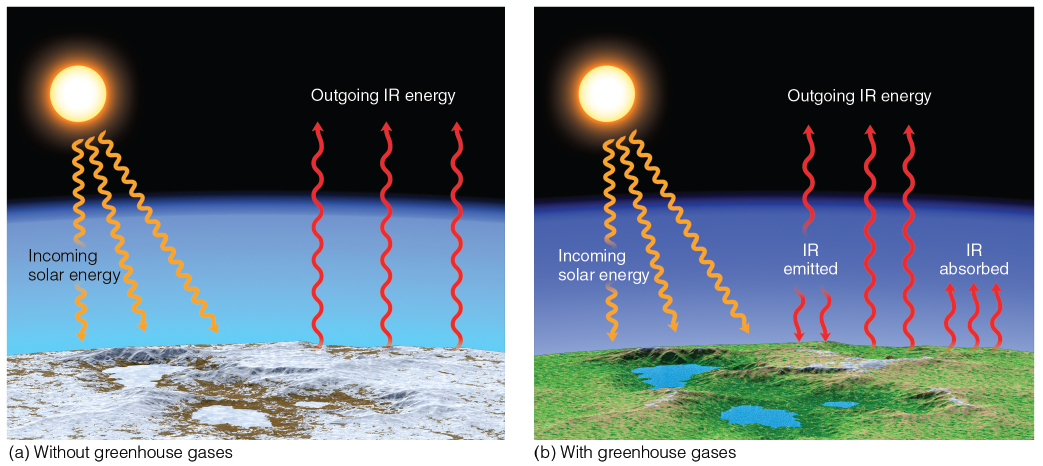
\includegraphics[width=1\linewidth]{figures/Figure132} 

}

\caption{Caption}\label{fig:GHG}
\end{figure}

\section{Energy balance}\label{energy-balance}

\subsection{Radiation balance}\label{radiation-balance}

When making an energy balance of the planet, we consider the solar
constant. This is the energy that we continuously receive from the sun
at the top of the atmosphere (= on average during the day we would
measure at the top of the atmosphere 1360 W per square meter).

\begin{figure}

{\centering 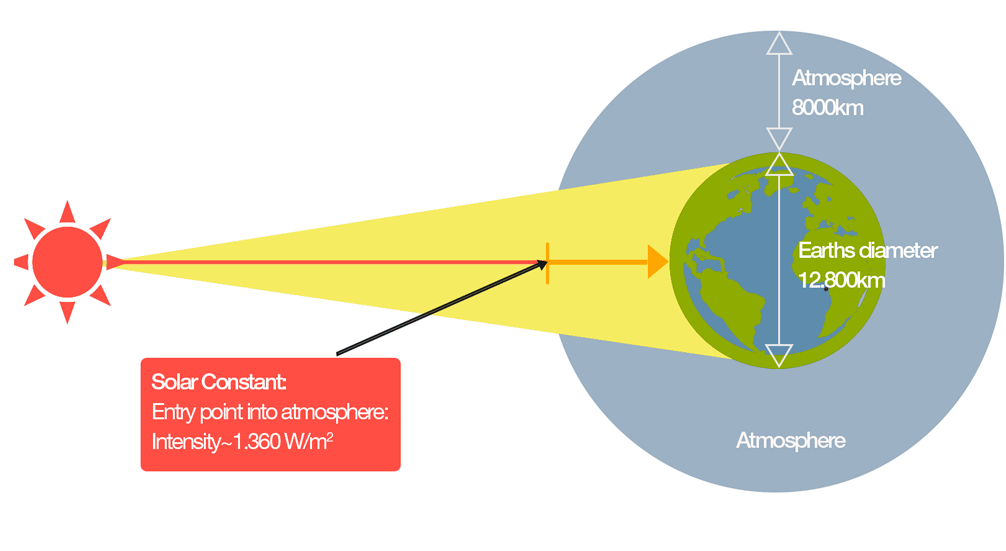
\includegraphics[width=0.6\linewidth]{figures/Figure133} 

}

\caption{Caption}\label{fig:RadBalance}
\end{figure}

As we have seen before, when this energy from the sun enters our
atmosphere there is interaction with molecules in the atmosphere
(diffusion, reflection, etc). Firstly we make a radiation balance and
secondly we make an energy balance. When making the radiation balance we
calculate how much radiation energy the earth, or for example a
grassland, receives and loses. We are calculating the \textbf{net
radiation}, what is left at the earth surface. The radiation balance is
made up off a shortwave (\((1-α) S_t\)) and a longwave radiation balance
(\(L_d – σ T^4\)). The shortwave balance is the total shortwave
radiation you measure with a pyranometer minus the reflected shortwave
radiation. The reflected shortwave radiation is determined by the
\textbf{albedo} (α), the reflectivity of the earth surface. The longwave
balance is the balance of infrared longwave radiation. There is longwave
radiation because objects with a temperature higher than 0 K emit
radiation and relatively cold objects (such as the clouds and molecules
in the atmosphere (\(L_d\)) and the earth surface (\(σ T^4\))) emit
longwave radiation. Finally, the net radiation balance is:

\begin{equation} 
  R_n = (1 - \alpha)S_t + L_d - \sigma T_0^{4}
  \label{eq:EqNetRadiation}
\end{equation}

The net radiation (the energy the system receives -- energy the system
loses) is the radiation which is available for the system to for example
heat the air or for evaporation.

\begin{figure}

{\centering 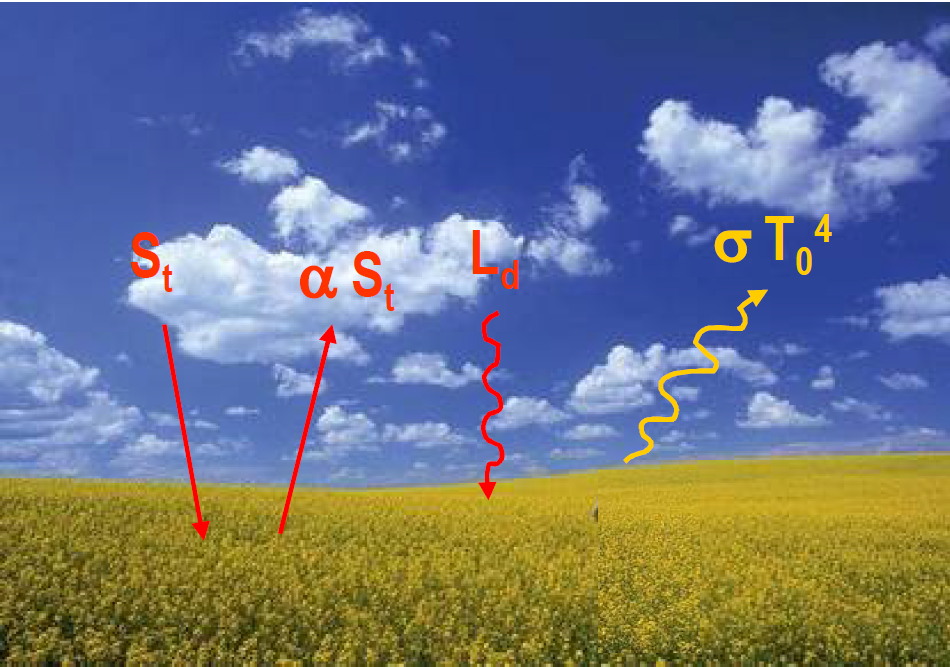
\includegraphics[width=0.5\linewidth]{figures/Figure134} 

}

\caption{Caption}\label{fig:RadiationAlbedo}
\end{figure}

The \textbf{albedo}, the reflectivity of the earth surface, is variable
and depends on the color of a surface. Forests (dark) and water surfaces
have a low albedo (they absorb a lot) while snow has a really high
albedo (reflects a lot). Albedo measured with satellites (e.g.~MODIS
albedo) show us that the highest albedos can be found in places covered
with snow and ice or in the desert, while places with a lot of
vegetation like forests in the tropics or temperate areas have a low
albedo.

\begin{figure}

{\centering 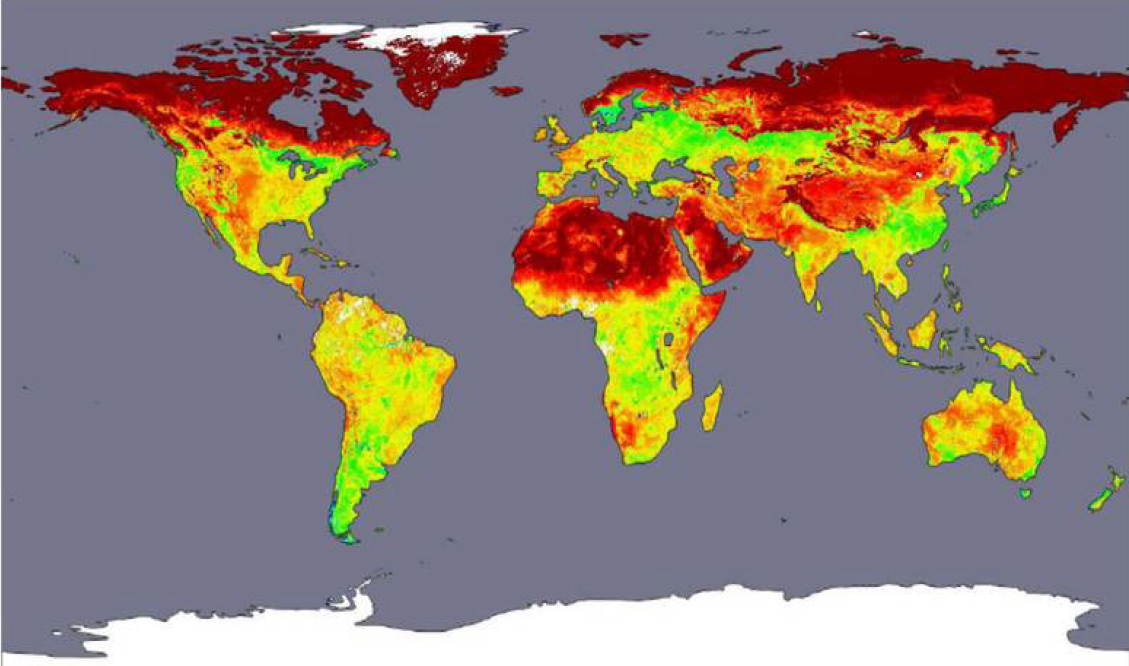
\includegraphics[width=0.5\linewidth]{figures/Figure135} 

}

\caption{Caption}\label{fig:albedo}
\end{figure}

\pagebreak

\begin{center}
\captionof{table}{Typical albedo of various surfaces*}
\label{table:albedos}

\begin{center}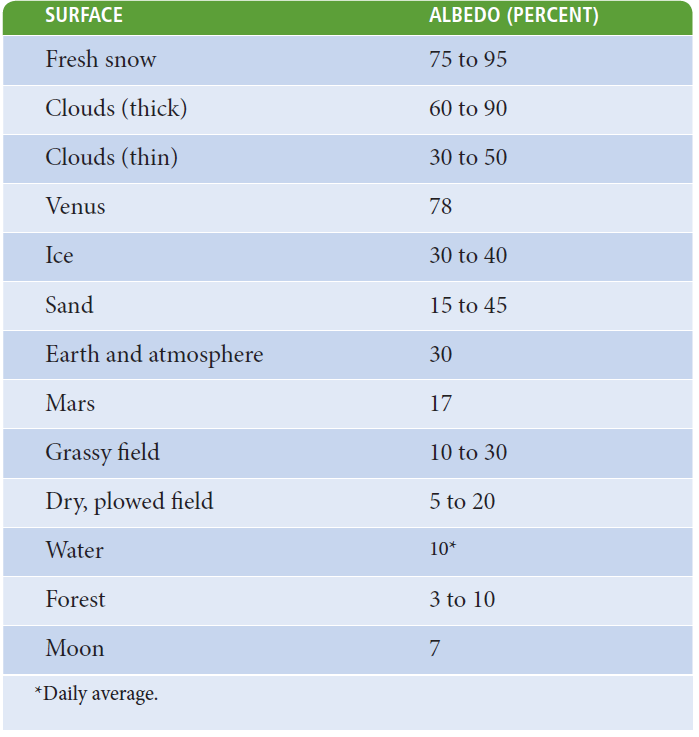
\includegraphics[width=0.8\linewidth]{figures/Table13} \end{center}
\end{center}

The next two figures are examples of the diurnal cycle of the components
of the radiation balance, where we can see the different components
change during the day. At night there is no shortwave radiation from the
sun. When the sun rises the incoming shortwave radiation increases
reaching a maximum at noon. The reflected shortwave radiation is a
fraction (α) of the incoming shortwave radiation. The outgoing and
incoming longwave radiation are quite constant (increasing a little bit
when the surface and air heat up during the day). Most importantly,
there is a \textbf{longwave deficit}, which means less longwave
radiation is received than lost. So, during the night the earth is
losing energy (no incoming shortwave, only longwave deficit) while
during the day energy is won, when the net shortwave radiation (surface
between the two shortwave curves) is larger than the longwave deficit.

\begin{figure}

{\centering 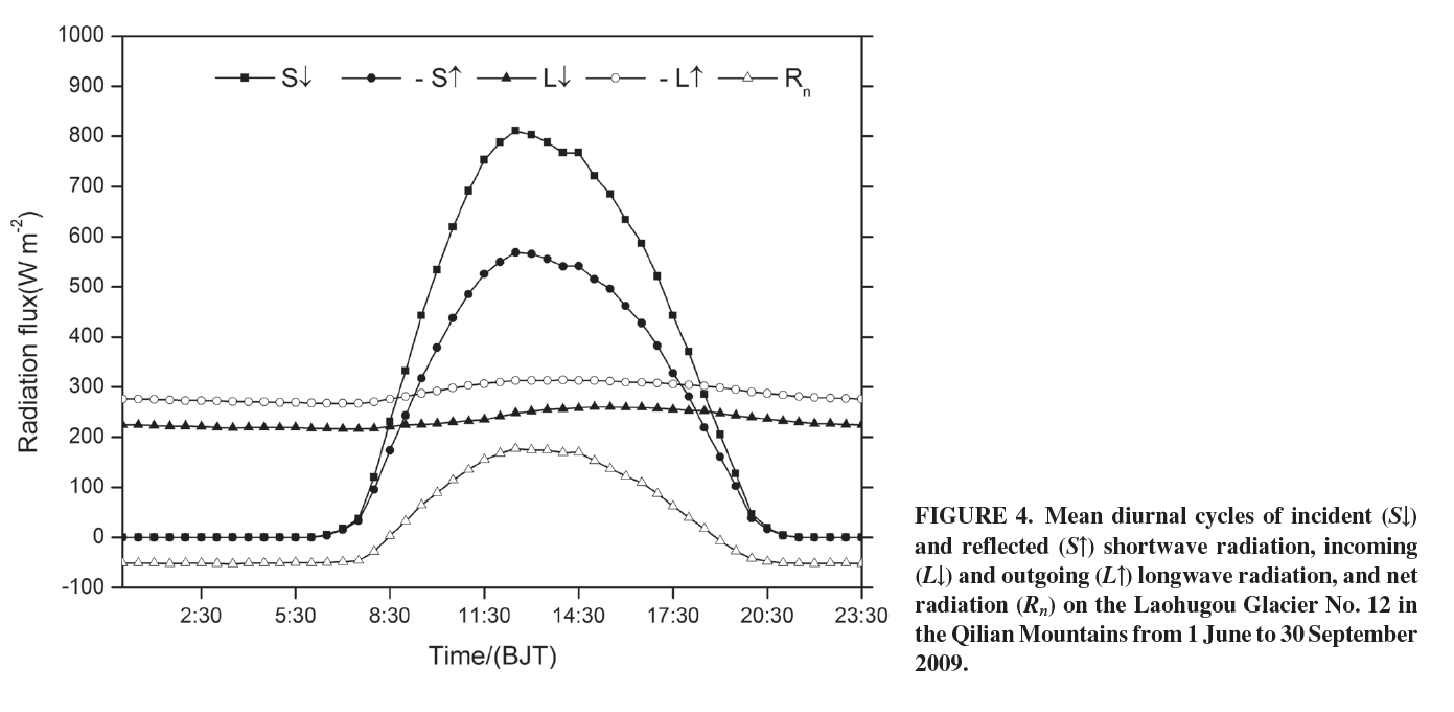
\includegraphics[width=0.77\linewidth]{figures/Figure136} 

}

\caption{Caption}\label{fig:RadiationCycle}
\end{figure}

\begin{figure}

{\centering 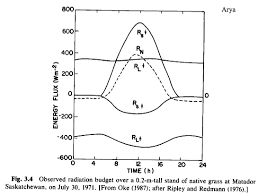
\includegraphics[width=0.9\linewidth]{figures/Figure137} 

}

\caption{Caption}\label{fig:RadiationCycle2}
\end{figure}

When we make the \textbf{radiation balance} for the planet with incoming
solar constant equalling 100 units, we see that only 51 units will reach
the earth because 30 units are reflected in the atmosphere, by clouds or
the earth surface and 19 units are absorbed by the atmosphere and
clouds. This is the average radiation balance of the earth (because
there is a large variation in local rardiation balances for different
places and at different moments in time).

\begin{figure}

{\centering 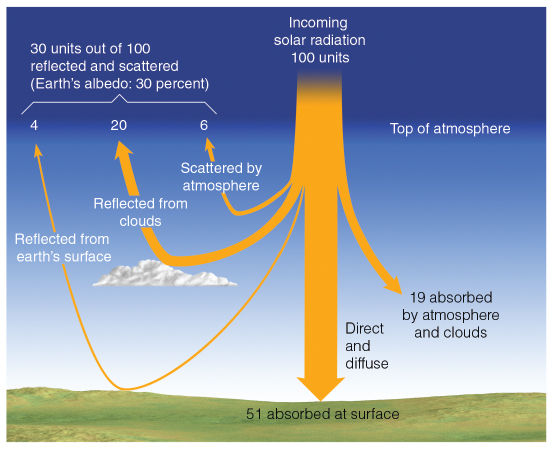
\includegraphics[width=0.65\linewidth]{figures/Figure138} 

}

\caption{Caption}\label{fig:RadiationBal}
\end{figure}

\subsection{Energy balance}\label{energy-balance-1}

The net radiation we calculate from the radiation balance is part of the
input of the energy balance.

\begin{equation} 
  R_n + \cancel{M} = \lambda E + H + G + S
  \label{eq:EqEnergyBalance}
\end{equation}

The \textbf{energy balance of the earth} describes what happens with the
\textbf{net radiation} that the earth receives from the sun. So on the
left side we have the energy gain and on the right side we have the
energy loss. You can make this energy balance for an object (house, the
hman body, \ldots{}), an ecosystem, for a region or for the whole
planet. Another energy input could be metabolism but this is neglected
in an ecosystem because the metabolic energy (for example from
photosynthesis and respiration reactions) is only a small fraction of
the total energy. The energy input is measured with a \textbf{net
radiation sensor}. Energy is lost through \textbf{latent heat} (λE,
evaporation), \textbf{sensible heat} (H, increasing air temperature),
through the \textbf{ground heat flux} (G, increasing soil temperature)
or it is \textbf{stored} in the system (S, residual storage term because
difficult to measure). These components are expressed in Watt per square
meter or energy flux per second (\(W m^{-2}\) or \(J s^{-1} m^{-2}\)).
The latent and sensible heat are measured using the eddy covariance (see
later in this course). Depending on the vegetation and water
availability more energy will go to evaporation or increasing the air
temperature. This is why a forest is cooler as more energy goes to
evaporation than heating the forest compared to other systems with less
vegetation. So, the energy balance is based on the conservation of
energy (energy gained has to go somewhere). On the long term the ground
heat flux and the storage term can be neglected in the energy balance as
everything that is taken up during the summer is released during the
winter.

This figure shows the average energy balance of the planet which is more
or less in balance. It is not in balance in certain places or on certain
points of time, this is why we continuously have temperature and weather
variations. But on average the system is quite stable with a net balance
at different levels (at the top of the atmosphere, at the earth
surface). The shortwave balance is the shortwave energy received and
reflected (like in the radiation balance) but the longwave balance also
includes the latent and sensible heat in addition to the longwave
radiation.

\begin{figure}

{\centering 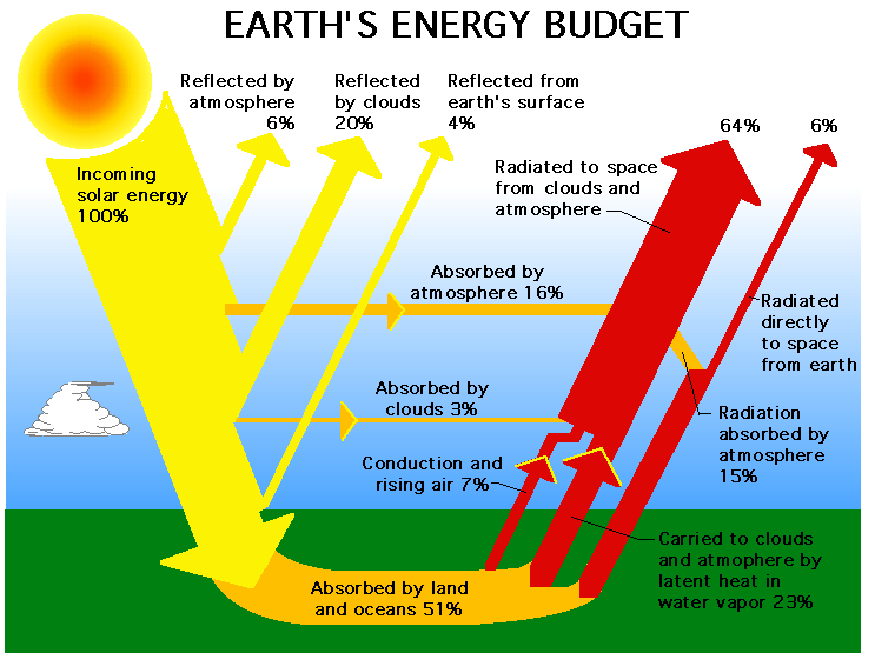
\includegraphics[width=0.7\linewidth]{figures/Figure139} 

}

\caption{Caption}\label{fig:EnergyBudget}
\end{figure}

The energy budget can be considered in different ways (see figures, say
the same thing but with different numbers). The last figure is not based
on 100 units of solar radiation coming in, but on 341 \(W m^{-2}\) which
is the average incoming solar radiation over a full year globally.

\begin{figure}

{\centering 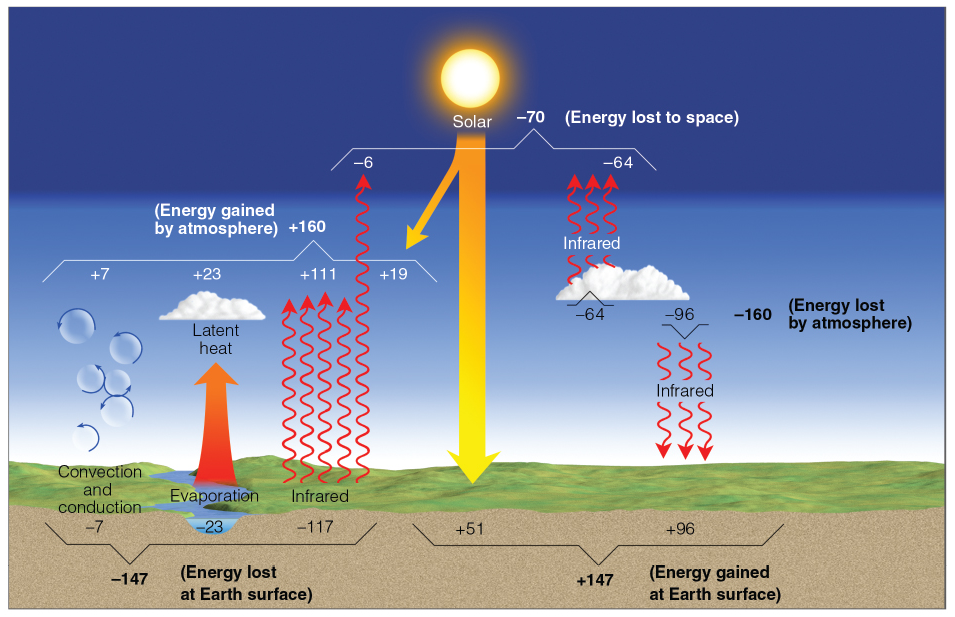
\includegraphics[width=0.8\linewidth]{figures/Figure140} 

}

\caption{Caption}\label{fig:EnergyBudget2}
\end{figure}

\begin{figure}

{\centering 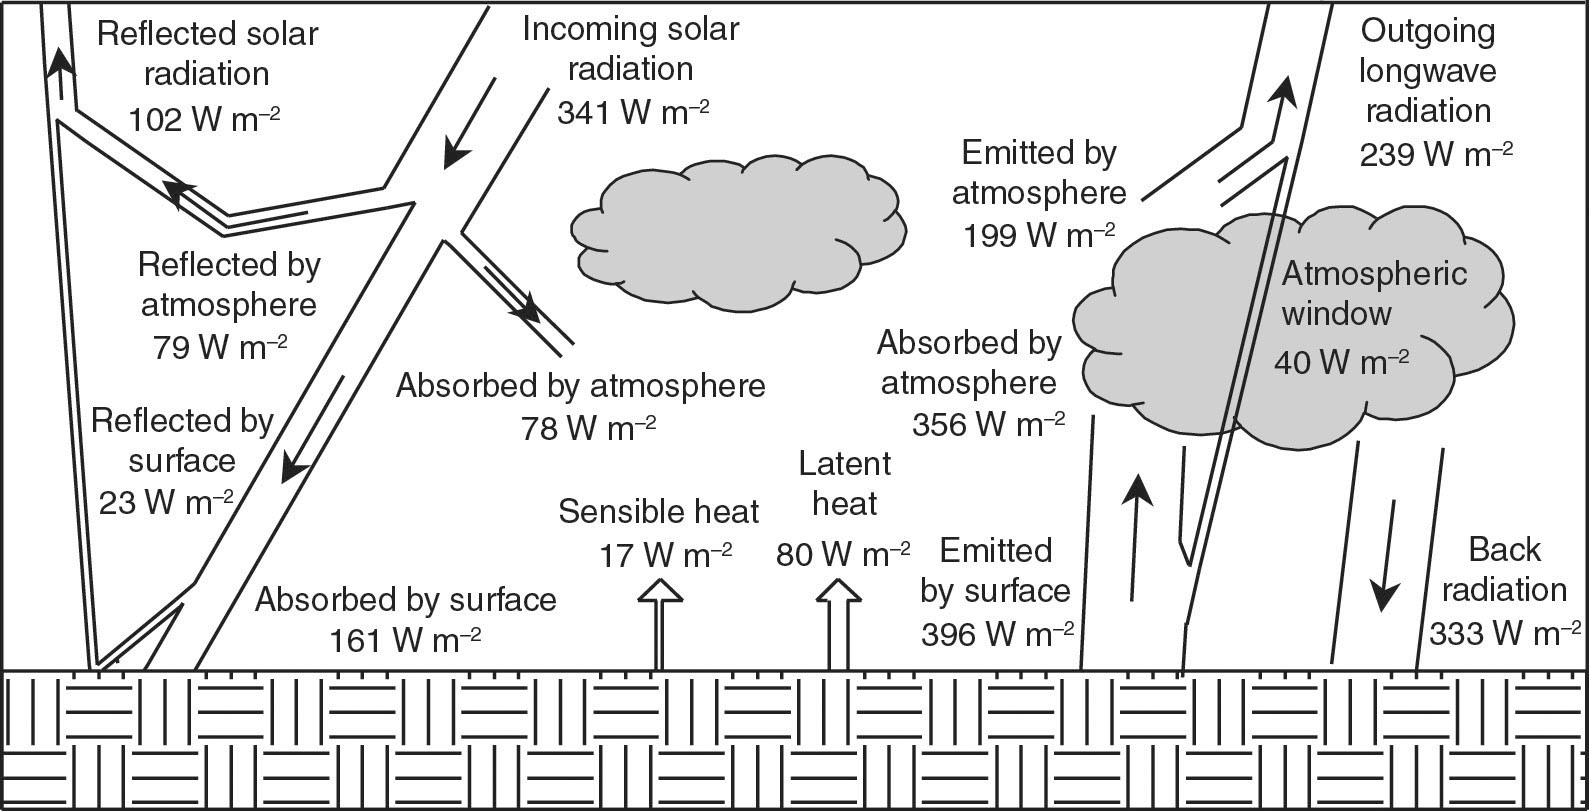
\includegraphics[width=0.7\linewidth]{figures/Figure141} 

}

\caption{Caption}\label{fig:EnergyBudget3}
\end{figure}

So the energy balance of the earth is on average in balance but this
\textbf{balance can shift (Climate change)}. Climate change (natural or
anthropogenic) is always related to one of three factors:
\textbf{radiation, atmospheric chemistry and albedo}. Solar radiation
(the input of the energy balance) can change in time when the sun is
more or less active, or because of changes in the geometry of the earth
and the sun (i.e.~Milankovich cycles). The atmospheric composition can
change which is mainly related to anthropogenic factors, greenhouse
gases, but also aerosols. The albedo, the reflectivity of the earth
surface, can change in time (vegetation cover, urbanisation, melting
polar ice caps). So the energy balance is in balance when considering
years but can change on the long term.

\begin{figure}

{\centering 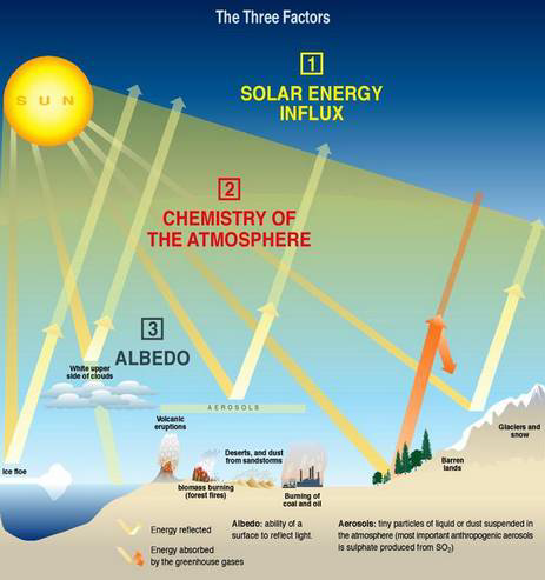
\includegraphics[width=0.6\linewidth]{figures/Figure142} 

}

\caption{Caption}\label{fig:EnergyBudget4}
\end{figure}

However, locally there is no balance (there is an \textbf{imbalance
according to latitude}). Locally, we receive more energy at the tropics
and less at the poles. Long wave deficit is larger at the equator
because the surface is hotter but net we still get more energy at the
equator and lose energy at the poles. So there is a continuous surplus
at the tropics and deficit at the poles. Therefore, there are continuous
heat transfers from the equator to the poles which drives the climate
system.

\begin{figure}

{\centering 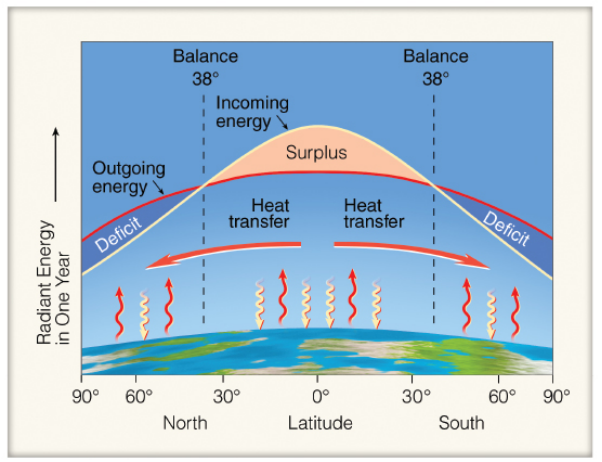
\includegraphics[width=0.7\linewidth]{figures/Figure143} 

}

\caption{Caption}\label{fig:EnergyBudget5}
\end{figure}

\section{Extra: Aurora borealis}\label{extra-aurora-borealis}

Polar light is a phenomenon which you can observe in northern areas
(aurora borealis) or on the south pole (aurora australis). It is a
visual effect related to the magnetic field of the earth. Solar storms
emit charged particles. These particles are deflected and reach the
atmosphere near the poles. They react with molecules in the atmosphere
which then are excited. When the electrons fall back, they emit light
(polar light).

\begin{figure}

{\centering 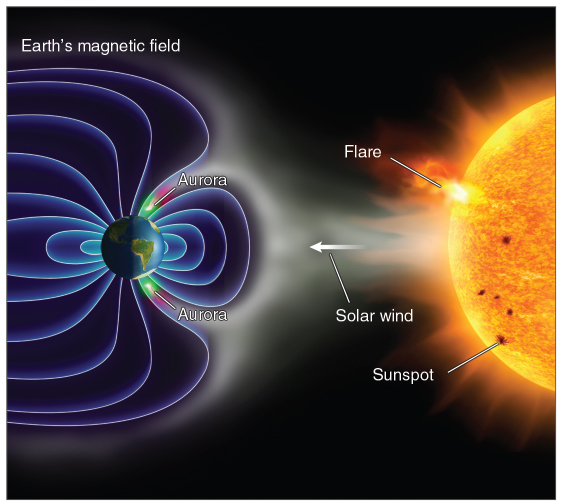
\includegraphics[width=0.5\linewidth]{figures/Figure144} 

}

\caption{Caption}\label{fig:borealis}
\end{figure}

\begin{figure}

{\centering \includegraphics[width=0.5\linewidth]{figures/Figure145} 

}

\caption{Caption}\label{fig:borealis2}
\end{figure}

\begin{figure}

{\centering \includegraphics[width=0.5\linewidth]{figures/Figure146} 

}

\caption{Caption}\label{fig:borealis3}
\end{figure}

\chapter{Temperature, humidity and
clouds}\label{temperature-humidity-and-clouds}

\chaptermark{Temp}

\section{Seasonal temperature
variation}\label{seasonal-temperature-variation}

Temperature is a measure for the \textbf{kinetic energy} of the
atmosphere (more energy in the atmosphere, means a higher temperature).
We're going to talk about the variations in temperature, the seasonal,
diurnal and spatial temperature variations.

\subsection{Seasons: why?}\label{seasons-why}

There are seasons on earth because of the variation in solar radiation
in time. The main driving factor is the \textbf{tilted axis of the
earth} (the earth's axis is not perpendicular to the plane of the
earth's orbit around the sun, but is tilted). This results in a
variation of the amount of solar radiation throughout the year but also
depending on the location on earth. The amount of solar radiation
depends on the \textbf{solar angle} (lower sun, solar radiation is
spread over a larger surface, lower solar intensity and more scattering)
and on the \textbf{day light hours}. Both of these factors are
determined by the tilt of the earth's axis and the geometry of the
earth's path around the sun. This path is elliptical (so the earth is
not always at a same distance from the sun). It is the tilt which causes
the seasons e.g.~during summer here (northern hemisphere), we are
furthest away from the sun but tilted towards the sun which causes a
higher insolation (due to the solar angle and day light hours). During
the spring and autumn we are closer to the sun. The figure here is an
exaggeration of the elliptical path, in reality it looks more like a
circle which is compressed just a little. Moreover, the sun is not
located in the center of the ellipse so during the winter we are closer
to the sun than during the summer (in NH). This might all be
counterintuitive but shows that this distance to the sun is less
important than the inclination of the earth's axis. You would expect
that in the southern hemisphere the seasons are more pronounced because
they are closer to the sun during summer and further away during the
winter, however, this is compensated by the fact that the
\textbf{southern hemisphere is covered by a larger amount of water which
acts as a buffer}. Therefore, seasonality in temperature is less
pronounced in the Southern hemisphere.

\begin{figure}

{\centering \includegraphics[width=1\linewidth]{figures/Figure21} 

}

\caption{Caption}\label{fig:Seasons}
\end{figure}

\begin{figure}

{\centering \includegraphics[width=1\linewidth]{figures/Figure22} 

}

\caption{Caption}\label{fig:Seasons2}
\end{figure}

If the earth axis wouldn't be tilted, there wouldn't be any seasons.
Every day would be the same, would be like 20th of March or the 22nd of
September. But this is not the case, there is an inclination of about
23,5° which can vary a little over the years (see course Climate Change
Processes).

\begin{figure}

{\centering \includegraphics[width=1\linewidth]{figures/Figure23} 

}

\caption{Caption}\label{fig:Seasons3}
\end{figure}

On the 21st of June the angle of 90° is above the tropic of Cancer while
on the 22nd of September it is above the equator and on the 21st of
December it is above the tropic of Capricorn causing the dynamics of the
seasons.

\begin{figure}

{\centering \includegraphics[width=1\linewidth]{figures/Figure24} 

}

\caption{Caption}\label{fig:Seasons4}
\end{figure}

\begin{figure}

{\centering \includegraphics[width=1\linewidth]{figures/Figure25} 

}

\caption{Caption}\label{fig:Seasons5}
\end{figure}

Above the polar circles there is also a special situation where during
the summer the north pole has 24 hours daylight while during the winter
it has none. So exactly on the poles there's six months of day and six
months of night but going further away from the poles the shorter the
polar night.

\begin{figure}

{\centering \includegraphics[width=0.5\linewidth]{figures/Figure26} 

}

\caption{Caption}\label{fig:Seasons6}
\end{figure}

\subsection{Impact on insolation}\label{impact-on-insolation}

The above described variations have an impact on the total solar
radiation which is available. This is calculated from the intensity
multiplied by the daylength. The \textbf{intensity depends on the solar
angle and the daylength} also depends on the solar geometry. The figure
presents the insolation throughout the year for different locations on
earth (different latitudes). At 60°N (a little more north than Belgium)
we can see a typical strong \textbf{seasonal pattern} of insolation.
When going to the north pole (90°N) this pattern is more extreme (six
month with and without insolation). At 30°N (region around the Sahara),
there is also strong seasonality but there is not a deep decline in
winter due to the high solar angles. On the equator (0°N), and
everywhere between the tropic of Cancer and the tropic of Capricorn (=
the \textbf{tropics}), there is a completely different pattern, a
\textbf{bimodal pattern}, because the sun is perpendicular to the
equator at two times (September and March). On the equator the two peaks
are nicely divided but going to the tropics the peaks come closer to the
21st of June. This is the resulting seasonality in insolation but this
does not mean the temperatures will follow the same pattern. The
temperature is not only determined by the incoming solar radiation but
also by all the other factors of the radiation balance.

\begin{figure}

{\centering \includegraphics[width=0.8\linewidth]{figures/Figure27} 

}

\caption{Caption}\label{fig:Insolation}
\end{figure}

This figure shows the situation on the 21st of June (summer solstice).
The blue line presents the insolation at the top of the atmosphere while
the red line presents the insolation at the earth's surface, for the
different latitudes. At the top of the atmosphere the insolation
increases from the equator to 23.5°N where the sun is perpendicular to
the earth (so mainly the solar angle is the driving factor here). Going
further north the solar angle decreases again but the length of the day
increases causes the total insolation to keep increasing. At the poles
there is an extra increase because there is 24 hours sun there.
Therefore the highest insolation over a day is reached at the north
pole. However, at the earth surface the insolation decreases after the
initial peak because with a lower solar angle comes longer paths through
the atmosphere and a lot of scattering. At the poles there is also a lot
of reflection from the polar caps (losing insolation). Clouds also play
a role, they are the reason why the insolation increases between 23.5°N
and 30°N, because there are no clouds above the deserts lying in between
these latitudes while at 23.5°N there were clouds.

\begin{figure}

{\centering \includegraphics[width=0.8\linewidth]{figures/Figure28} 

}

\caption{Caption}\label{fig:Insolation2}
\end{figure}

The \textbf{radiation balance} is in balance globally but not locally
and not \textbf{according to latitude}. The net shortwave radiation is
shown in blue which is high at the equator and decreases to the poles.
The longwave radiation loss is shown in red and has two peaks at 23.5°N
and 23.5°S as these are the warmest regions (see Stefan-Boltzmann). This
results in a net \textbf{surplus at the equator} and a \textbf{deficit
at the poles}. To compensate, a continuous flux of energy is needed from
the equator to the poles which is realised through \textbf{ocean
currents, wind circulation and latent heat} (more evaporation at the
equator and more condensation at the poles). These three component each
transport 1/3 of the energy.

\begin{figure}

{\centering \includegraphics[width=0.9\linewidth]{figures/Figure29} 

}

\caption{Caption}\label{fig:Insolation3}
\end{figure}

\begin{figure}

{\centering \includegraphics[width=0.8\linewidth]{figures/Figure210} 

}

\caption{Caption}\label{fig:Insolation4}
\end{figure}

\subsection{Apparent path of the sun}\label{apparent-path-of-the-sun}

If we look at the geometry of the path of the earth around the sun from
the perspective of someone standing on the earth surface, we can see the
apparent path of the sun. If you stand on the north pole you see the sun
going in a circle, with this circle descending when winter is coming
closer. The closer to the equator the more perpendicular the sun will
relative to the earth. At the equator the sun will apparently rise
straight up with a little variation to the north or south depending on
the time of the year. This also causes the fact that in the tropics the
transition between day and night will be very fast.

\begin{figure}

{\centering \includegraphics[width=0.9\linewidth]{figures/Figure211} 

}

\caption{Caption}\label{fig:Path}
\end{figure}

\subsection{Solar geometry}\label{solar-geometry}

We can also quantify solar elevation by using the \textbf{zenith angle},
this is the angle between the zenith (line perpendicular on the earth
surface) and the Sun. The \textbf{altitude angle}, the angle between the
horizontal and the line to the Sun is also used. The \textbf{azimuth
angle} is measured as the angular distance from the north. These angles
can be calculated with the help of several formulas.

\begin{figure}

{\centering \includegraphics[width=0.8\linewidth]{figures/Figure212} 

}

\caption{Caption}\label{fig:SolarGeom}
\end{figure}

\begin{equation} 
  cos Z = sin B = sin \phi \cdot sin \delta + cos \phi \cdot cos \delta \cdot cos h
   \label{eq:Eqangles}
\end{equation}

\begin{itemize}
\tightlist
\item
  Z is the zenith angle
\item
  B is the altitude angle
\item
  φ is the latitude
\item
  ∂ is the solar declination of the earth (varies around 23°)
\item
  H is the solar hour angle (the angle between the solar noon and where
  it is at the moment of observation, it is expressed in ° or in hours,
  1 hour before solar noon the hour angle is -1 or -15°)
\end{itemize}

\begin{equation} 
  cos A_{sun} = \frac{\left(sin \delta \cdot cos \phi - cos \delta \cdot sin \phi \cdot cos h \right)} {sin Z}
   \label{eq:EqAsun}
\end{equation}

Asun is the azimuth angle.

The total amount of radiation received at the atmosphere is the
\textbf{solar constant} of 1370 Watt per square meter (seen before). We
can correct this for solar angle and the radius vector rv, relative
distance between the earth and sun, the relative ratio between the
current and average distance to the sun.

\begin{equation} 
   S_H = S_p cos Z
   \label{eq:Eqdist1}
\end{equation}

\begin{equation} 
   S_H = \frac{S_c}{r_v^{2}} cos Z
   \label{eq:Eqdist2}
\end{equation}

We can also calculate the total daylength, defined as the period during
which the sun is above the horizon. See more details during the
practical.

\begin{equation} 
   \frac{24}{\pi} cos^{-1}\left(-tan\phi \cdot tan \delta \right)
   \label{eq:Eqdaylength}
\end{equation}

\section{Daily (diurnal) temperature
variation}\label{daily-diurnal-temperature-variation}

The daily temperature variation is driven by the rotation of the earth
and the day-night pattern. The rotation of the earth causes the
alternation of day and night but also the rising and falling solar
elevation.

\subsection{Temperature profiles}\label{temperature-profiles}

When we measure the temperature at different heights above the ground we
see an \textbf{exponential profile} during a calm day while on a windy
day a \textbf{linear profile} is obtained because of the
\textbf{turbulence} and mixing of the different layers due the wind. On
a calm day this exponential profile is caused mainly by convection (hot
air bubbles are created at the earth surface due to the heating of the
ground by the sun, but very slow process) and a little bit by conduction
(only in the very low layers).

\begin{figure}

{\centering \includegraphics[width=1\linewidth]{figures/Figure213} 

}

\caption{Caption}\label{fig:TempProfile}
\end{figure}

During the night, cooling is strong at the earth surface (long wave
radiation is leaving the surface = radiational cooling), causing a
\textbf{nocturnal inversion}. This results in an increasing temperature
profile with the coolest, heaviest air at the surface (which does not
have the tendency to mix with the upper layers) and thus causes a stable
atmosphere. Therefore, when comparing day and night the
\textbf{temperature variation at the surface will be very large} (at
night, the lowest temperatures are reached while during the day the
hottest temperatures are obtained). This is why we don't measure the
temperature at the surface but at \textbf{1.5 m high in a thermometer
hut} (above the diurnal variation), so we can measure the variation from
day to day. The temperature also depends on humidity, wind, albedo,
vegetation, which is also why a thermometer is placed in a hut with
shielding so it is not determined by direct radiation. Also during the
night the profile is linear for a windy night and exponential when it is
a calm night.

\begin{figure}

{\centering \includegraphics[width=0.5\linewidth]{figures/Figure214} 

}

\caption{Caption}\label{fig:TempProfile2}
\end{figure}

\subsection{Temperature--radiation
link}\label{temperatureradiation-link}

This figure shows how the temperature will vary during a sunny day
(diurnal pattern of 24 hours) but it also shows the net radiation
balance (net shortwave incoming \& net long wave outgoing). The highest
temperatures on a sunny day are not reached at the solar noon but a few
hours later. The peak of temperature is not at the same time as the peak
of solar energy because the temperature is the result of the total
energy balance. During the day the incoming energy will be larger than
the outgoing energy (positive net energy), which means that also after
the solar noon the systems is receiving energy and thus keeps warming
the atmosphere. Only when the incoming solar energy is lower than the
outgoing energy (in the afternoon), there is a energy deficit and the
atmosphere starts cooling. The temperature will decline as long as the
outgoing energy is larger than the incoming energy, which is until a few
moments after the sun rises (the first moments after the sun rises the
incoming solar radiation is not yet enough to compensate the long wave
deficit). In the early morning the coolest temperature is measured. The
temperature profile is determined by the difference between incoming
solar energy and outgoing energy but the outgoing long wave energy
profile is also determined by the earth surface temperature. Therefore,
the peak in long wave deficit will also be in the afternoon when the
surface is hottest. In conclusion, temperature and radiation are linked
in both directions. On a cloudy day the incoming solar energy will
fluctuate more, causing the temperature (and thus the long wave deficit)
not to follow this nice, theoretic pattern.

\begin{figure}

{\centering \includegraphics[width=0.8\linewidth]{figures/Figure215} 

}

\caption{Caption}\label{fig:TempRad}
\end{figure}

\subsection{Thermal belt in valleys}\label{thermal-belt-in-valleys}

The temperature profile has an impact on agriculture. For example, at
night there will be advection (horizontal transport) of cold air
downhill in the valley while warm air is stays on top. But because the
temperature also decreases with height there will be a combination of
these two effects and the highest temperatures are reached in the
middle. This is called a \textbf{thermal belt}, a zone on hillsides
where there is a moderate climate (it doesn't really cool off that much
here) and where certain plants can grow which cannot grow below or above
this zone. Vineyards will typically be located in these zones (not on
the bottom of these valleys). Another consequence is that there is cold
and stable air on the bottom of the valley where smoke and pollution
will linger increasing the environmental and \textbf{pollution problem
of cities located in valleys}.

\begin{figure}

{\centering \includegraphics[width=0.8\linewidth]{figures/Figure216} 

}

\caption{Caption}\label{fig:ThermalBelt}
\end{figure}

\subsection{Crop protection}\label{crop-protection}

The peak of low temperature in the early morning can be a problem for a
lot of crops, especially in spring when the crops are growing.
Therefore, there are several methods to deal with this spring frost.
Firstly, there are \textbf{orchard heaters} which blow warm air but are
not energy efficient. Secondly, a smarter method is the use of
\textbf{wind generators} which cause turbulence and mixing of the cold
air with the warmer air above (changing the exponential temperature
profile into a linear profile with warmer temperatures near the ground).
Thirdly, there is a method where you spray the crops with water just
before the temperatures drop below freezing, which creates an
\textbf{ice coating} and releases latent heat. Lastly, \textbf{plastic
foils} are used to keep the heat inside (green house effect).

\section{Regional temperature
variation}\label{regional-temperature-variation}

\subsection{Main temperature controls}\label{main-temperature-controls}

The temperature varies worldwide (see world map which shows the average
temperature over 30 years). From this map we can derive the \textbf{four
main temperature controls} on earth. Firstly, the most important control
is the \textbf{latitude} (\textasciitilde{} solar angle, higher
latitudes are colder). However, this map is not linear with latitude
because of the three other temperature controls. Secondly, \textbf{land
and water} transition also play an important role (lines deflect near
land water transitions). Thirdly, \textbf{ocean currents} play an
important role and explain for example why it is warmer in Europe than
on the same latitude in North America. Lastly, \textbf{elevation}
explains some anomalies such as the one near the Himalayas, Alpes, Rocky
mountains and Andes. These four factors determine for the most part
which temperatures there are on earth. But of course, there are also
local factors which determine the temperature locally and regionally.

\begin{figure}

{\centering \includegraphics[width=1\linewidth]{figures/Figure217} 

}

\caption{Caption}\label{fig:MAT}
\end{figure}

\subsection{Global isotherm maps (°F)}\label{global-isotherm-maps-f}

On this global isotherm map for January we can see the highest
temperatures south of the equator. We see the \textbf{isotherms are
closer to each other in the northern hemisphere} (e.g.~strong
temperature gradients and thus very variable weather). In the contrary
in July, the isotherms have shifted up but also the isotherms are
further away from each other meaning weather will be more stable.

We can also see that near \textbf{water-land transitions}, there are
kinks in the isotherms. This is caused by the different energy balance
between land and water due to the higher heat capacity of water. But
these kinks are also related to the \textbf{ocean currents} (e.g.~higher
temperatures near Europe caused by the golf stream). Lastly, we see that
in the \textbf{southern hemisphere the situation is stable throughout
the year} (the isotherms are practically parallel and not close
together). This is because there is significantly less land mass in the
southern hemisphere.

\begin{figure}

{\centering \includegraphics[width=1\linewidth]{figures/Figure218} 

}

\caption{Caption}\label{fig:Isotherm}
\end{figure}

\begin{figure}

{\centering \includegraphics[width=1\linewidth]{figures/Figure219} 

}

\caption{Caption}\label{fig:Isotherm2}
\end{figure}

\section{Air temperature data}\label{air-temperature-data}

\subsection{Temperature scales}\label{temperature-scales}

\begin{equation} 
   K = ^{\circ}C + 273.13
   \label{eq:EqK}
\end{equation}

\begin{equation} 
   ^{\circ}C = 5/9 \left(^{\circ}F - 32 \right)
   \label{eq:EqF}
\end{equation}

\begin{figure}

{\centering \includegraphics[width=1\linewidth]{figures/Figure220} 

}

\caption{Caption}\label{fig:TempScale}
\end{figure}

\subsection{Thermometer huts}\label{thermometer-huts}

How do we measure these air temperatures? In standard circumstances,
temperature is measured in a thermometer hut which is well ventilated
and cut off from radiation. This thermometer hut is also placed on a
standard height to be above the diurnal temperature variations. In the
past this was done manually (someone went out two times a day to measure
the temperature). With a minimum-maximum thermometer the minimum and
maximum temperature of the last 24 hours can also be measured.

\begin{figure}

{\centering \includegraphics[width=0.7\linewidth]{figures/Figure221} 

}

\caption{Caption}\label{fig:Huts}
\end{figure}

\subsection{MAT (Mean annual temperature) vs
seasonality}\label{mat-mean-annual-temperature-vs-seasonality}

What do we do with this data? Often the mean annual temperature (MAT) of
a location is used. But this does not say everything about the climate.
For example, two different locations can have the same mean annual
temperature but completely different climates.

\begin{figure}

{\centering \includegraphics[width=0.7\linewidth]{figures/Figure222} 

}

\caption{Caption}\label{fig:MAT1}
\end{figure}

\subsection{Growing degree days}\label{growing-degree-days}

Growing degree days is a cumulative temperature sum. You choose a basis
temperature (for example 0°) and measure the maximum temperature
everyday (for example 5° today, 10° tomorrow, 6° the day after that).
Then you make the cumulative sum of the differences between the maximum
temperatures and the basis temperature (so 5+10+6=21 degree days).
During the growing season you can further accumulate this temperature
sum which is used to study or estimate different phenological phenomena
of plants (for example, you need a sum of 1200-1300 to harvest certain
crops).

\begin{center}
\captionof{table}{Estimate Growing degree days for certain naturally grown agricultural crops to reach maturity}
\label{table:GDD}

\begin{center}\includegraphics[width=0.8\linewidth]{figures/Table21} \end{center}
\end{center}

\subsection{Wind chill index (WCI)}\label{wind-chill-index-wci}

The temperature we feel depends on the wind and is determined through
the wind chill index. Higher wind speeds gives us lower wind chill index
(so it feels colder when there is more wind).

\begin{center}
\captionof{table}{Wind-chil equivalent temperature}
\label{table:WC}

\begin{center}\includegraphics[width=0.8\linewidth]{figures/Table22} \end{center}
\end{center}

\section{Atmospheric moisture
(psychometry)}\label{atmospheric-moisture-psychometry}

The study of air humidity is also called psychometry.

\subsection{Three phases of water}\label{three-phases-of-water}

Water is present in the air in three phases: solid (ice), liquid (water
droplets), gas (water vapor). Above a water surface there is a dynamic
equilibrium, where water evaporates and condensates continuously.

\begin{figure}

{\centering \includegraphics[width=0.7\linewidth]{figures/Figure223} 

}

\caption{Caption}\label{fig:Phases}
\end{figure}

\begin{figure}

{\centering \includegraphics[width=0.7\linewidth]{figures/Figure224} 

}

\caption{Caption}\label{fig:Phases2}
\end{figure}

\subsection{Saturation and
condensation}\label{saturation-and-condensation}

If you have a closed jar with water and air, an equilibrium will be set,
where there will be and equal amount of evaporation and condensation. In
this situation, the air will be \textbf{saturated} with water vapour
(100\% relative humidity). Condensation happens on a surface, typically
\textbf{condensation nuclei} (so when water vapor collides with these
particles they could condense on them).

\begin{figure}

{\centering \includegraphics[width=0.7\linewidth]{figures/Figure225} 

}

\caption{Caption}\label{fig:Saturation}
\end{figure}

This condensation will happen more easily in cold air because in warm
air there is more kinetic energy and the water vapor won't stick as
easily to the nuclei.

\begin{figure}

{\centering \includegraphics[width=0.7\linewidth]{figures/Figure226} 

}

\caption{Caption}\label{fig:Saturation2}
\end{figure}

\subsection{Humidity terminology}\label{humidity-terminology}

How do we define air humidity? There are several definitions when
looking at a parcel of air to define how much water is present. Firstly,
there is \textbf{absolute humidity}, this is the mass of water vapour
per volume of air (g/m³). But if the air warms, the volume of the parcel
will increase and the absolute humidity will decrease while the amount
of water molecules stays the same. Secondly, the \textbf{specific
humidity}, is the mass of water per total mass of air (g/kg). In
contrary to the absolute humidity the specific humidity stays the same
when the temperature increases (and is therefore preferred in
meteorology). Thirdly, the \textbf{mixing ratio} is the mass of water
per mass of dry air and is mainly used in atmospheric chemistry
(studying pollutants).

\begin{figure}

{\centering \includegraphics[width=0.7\linewidth]{figures/Figure227} 

}

\caption{Caption}\label{fig:Humidityterm}
\end{figure}

\begin{figure}

{\centering \includegraphics[width=1\linewidth]{figures/Figure228} 

}

\caption{Caption}\label{fig:Humidityterm2}
\end{figure}

\begin{figure}

{\centering \includegraphics[width=1\linewidth]{figures/Figure229} 

}

\caption{Caption}\label{fig:Humidityterm3}
\end{figure}

This figure shows the specific humidity on earth in g/kg air per
latitude. Typically, there is a latitudinal pattern with high specific
humidity at the equator and decreasing specific humidity to the poles.
It tells us something about the exact amount of moisture there is in the
air, so also above dry areas (e.g.~savannas) high values are obtained
even though the air doesn't feel humid. How we perceive humidity is
better presented with the relative humidity (see later).

\begin{figure}

{\centering \includegraphics[width=0.5\linewidth]{figures/Figure230} 

}

\caption{Caption}\label{fig:Humidityterm4}
\end{figure}

This figure shows the global pattern of specific humidity and shows the
areas with more moisture in the air, typically more above oceans
compared to land and typically more above the equator than further away
from it. This is the situation in July (summer in northern hemisphere),
in the winter it will be shifted downwards because then there is more
evaporation above the oceans in the southern hemisphere.

\begin{figure}

{\centering \includegraphics[width=0.9\linewidth]{figures/Figure231} 

}

\caption{Caption}\label{fig:Humidityterm5}
\end{figure}

\subsection{Vapour pressure}\label{vapour-pressure}

Vapour pressure is the partial pressure of water in a gas mixture (in
this case, the air). The \textbf{actual vapour pressure} is the vapour
pressure we observe at the moment. \textbf{Saturated vapour pressure} is
the vapour pressure in saturated air (closed container) and depends on
the temperature. At different temperatures there will be different
saturated vapour pressures. At lower temperatures, condensation is
slower (lower flux) so you also need less evaporation to be in
equilibrium. The saturated vapour pressure increases exponentially with
temperature (see figure). Below 0°C (above ice or above super cooled
water) there is also a vapour pressure. The curve is different for ice
compared to super cooled water because sublimation of ice to gas is
slower than evaporation of water to gas. The current vapour pressure is
also the pressure measured in an open container (see figure).

\begin{figure}

{\centering \includegraphics[width=0.9\linewidth]{figures/Figure232} 

}

\caption{Caption}\label{fig:VP}
\end{figure}

The \textbf{Mollier diagram} (psychrometric chart) shows the saturated
vapour pressure as a function of the temperature (line at RH = 100). It
also shows different relative humidities which are equal to the current
vapour pressure divided by the saturated vapour pressure and thus, also
depends on the temperature. If you have a closed container with a
certain actual vapour pressure, and if you increase the temperature, the
actual vapour pressure stays the same but the relative humidity
decreases. This is because the saturated vapour pressure increases (warm
air can hold more water vapour than cold air). On a Mollier diagram you
can also determine the \textbf{dry and wet bulb temperature}. The wet
bulb temperature is the temperature you measure with a thermometer which
is covered with a wet cloth. The dry bulb temperature is what you
measure with a normal thermometer. If you know these two temperatures
you can determine the (\textbf{relative}) \textbf{air humidity} using
the Mollier diagram. Also the \textbf{dew point}, the temperature at
which condensation happens, can be determined.

\begin{figure}

{\centering \includegraphics[width=0.9\linewidth]{figures/Figure233} 

}

\caption{Caption}\label{fig:Mollier}
\end{figure}

\begin{figure}

{\centering \includegraphics[width=0.6\linewidth]{figures/Figure234} 

}

\caption{Caption}\label{fig:Mollier2}
\end{figure}

\subsection{Relative humidity and
dewpoint}\label{relative-humidity-and-dewpoint}

On a sunny day without rain (no water input) there is an inverse
relationship between the temperature and the relative humidity. Relative
humidity is important in meteorology because it really tells something
about how we experience the air humidity. It is not only how we
experience it but also how plants experience it. It also determines
evapotranspiration. Typically, the highest relative humidity is obtained
when the temperature is lowest (early in the morning).

\begin{figure}

{\centering \includegraphics[width=1\linewidth]{figures/Figure235} 

}

\caption{Caption}\label{fig:dewpoint}
\end{figure}

Dew point is the temperature to which air would have to be cooled for
saturation/condensation to occur (with no change in air pressure or
moisture content). Dew point is also a measure for absolute water vapour
content in the air because the higher the dew point the faster
condensation will occur when the air cools. A higher dew point means
more humid air, a higher water content in the air. This is why dew point
is also important in meteorology. In the desert where there is a dew
point of 10°C there is more water in the air in absolute terms than at
the poles where there is a dew point of -2°C although it may feel the
other way around.

\begin{figure}

{\centering \includegraphics[width=1\linewidth]{figures/Figure236} 

}

\caption{Caption}\label{fig:dewpoint2}
\end{figure}

\subsection{Heat index}\label{heat-index}

The air humidity also determines how we experience temperature. So how
we experience temperature is not only determined by the wind chill but
also by the air humidity. A higher humidity results in a higher
temperature experience (see heat index) because your body has more
difficulty to transpire in humid air.

\begin{figure}

{\centering \includegraphics[width=1\linewidth]{figures/Figure237} 

}

\caption{Caption}\label{fig:HI}
\end{figure}

\section{Condensation: dew, fog and
clouds}\label{condensation-dew-fog-and-clouds}

\subsection{Condensation on surface}\label{condensation-on-surface}

Condensation always happens on a surface, when the dew point is reached
(and thus depends on the air humidity). When the temperature cools till
the dew point condensation, \textbf{deposition or rime} formation
occurs. Condensation on the earth surface can result for example in the
formation of \textbf{dew}. This happens in the morning because the loss
of long wave radiation can cool down the air till the dew point and
condensation happens. This cooling (and thus dew formation) is typically
strong on clear calm nights (no clouds so a lot of longwave radiation
loss and no turbulence which creates the exponential temperature
decrease). \textbf{Frozen dew} are droplets which form and subsequently
freeze while rime is water vapour which freezes onto the surface
directly.

\begin{figure}

{\centering \includegraphics[width=1\linewidth]{figures/Figure238} 

}

\caption{Caption}\label{fig:Condew}
\end{figure}

\subsection{Condensation nuclei}\label{condensation-nuclei}

In the atmosphere, condensation happens on \textbf{condensation nuclei}
(e.g.~aerosols, small particles in the air). These condensation nuclei
can be \textbf{hygroscopic} (attract water) resulting in faster
condensation. They can also be \textbf{hydrophobic} (repel water) but
then it has to be even colder in order for condensation to take place on
the particle. Condensation nuclei are typically particles which are
\textbf{smaller than 0.1 µm} and are present in the atmosphere in a
density of 100 - 1000 particles/cm³. They can be classified according to
size but the majority are the smallest particles (\textless{}0.1 µm).

\begin{figure}

{\centering \includegraphics[width=0.8\linewidth]{figures/Figure239} 

}

\caption{Caption}\label{fig:Nuclei}
\end{figure}

\begin{center}
\captionof{table}{Characteristic sizes and concentration of condensation nuclei and cloud droplets}
\label{table:droplet}

\begin{center}\includegraphics[width=0.8\linewidth]{figures/Table23} \end{center}
\end{center}

\subsection{Haze}\label{haze}

These condensation nuclei induce condensation, water droplets that
linger in the atmosphere. If these are low above the ground, there is
\textbf{haze and fog}. The difference is determined by the visibility.
If you cannot see farther than 1 km then we talk about fog. If you can
see farther than 1 km then we talk about haze. Haze is also split up in
dry and wet haze according to the relative humidity which is less than
75\% and more than 75\% respectively. Fog and haze are also typically
formed in the morning when a cold layer of air is obtained due to
radiational cooling and the dew point is reached.

\begin{figure}

{\centering \includegraphics[width=0.8\linewidth]{figures/Figure240} 

}

\caption{Caption}\label{fig:Haze}
\end{figure}

\subsection{Fog types}\label{fog-types}

Fog can be classified into four groups. The phenomenon is the same,
condensation in the air layer above the earth surface, but the cause is
different.

\begin{figure}

{\centering \includegraphics[width=0.8\linewidth]{figures/Figure241} 

}

\caption{Caption}\label{fig:Fog}
\end{figure}

The most important type is \textbf{radiation fog} (ground fog) which is
caused by radiational cooling (longwave cooling at night). This is
typically fog where we can see above it (e.g.~radiational fog in a
valley due to advection). This fog typically disappears during the
morning because the droplets evaporate again to the sun.

\begin{figure}

{\centering \includegraphics[width=0.8\linewidth]{figures/Figure242} 

}

\caption{Caption}\label{fig:Fog2}
\end{figure}

The second type of fog is \textbf{advection fog} (horizontal transport)
which is formed when humid air moves over a cold surface and cools down
and condenses. In Europe this can typically be found above the British
isles, Ireland and Scotland. In winter the land is colder than the ocean
and relatively warm moist air moves over Ireland/Scotland which then
cools down and condensates forming advection fog. The best-known example
of advection fog is the fog in the bay of San Francisco. This bay
receives rivers that come from inland/mountains with cold water. If warm
ocean air goes over this bay this air cools off and forms a fog.

\begin{figure}

{\centering \includegraphics[width=0.8\linewidth]{figures/Figure243} 

}

\caption{Caption}\label{fig:Fog3}
\end{figure}

The third type of fog is \textbf{upslope fog} which is found in mountain
areas, where the wind pushes air up the mountain and the air cools off
and condenses.

\begin{figure}

{\centering \includegraphics[width=0.8\linewidth]{figures/Figure244} 

}

\caption{Caption}\label{fig:Fog4}
\end{figure}

The last type of fog is \textbf{evaporation fog}/\textbf{mixing fog} and
is the result of the mixing of hot humid air and cold air. The humid air
cools off and condenses. This fog is typically formed after a heavy rain
fall in summer when water evaporates from the wet road and mixes with
the colder air above and condenses. Evaporation fog also arises above
geysers where the warm humid air above the geyser mixes with the colder
air around it and condenses. Evaporation fog is typically a local
phenomenon.

\begin{figure}

{\centering \includegraphics[width=0.8\linewidth]{figures/Figure245} 

}

\caption{Caption}\label{fig:Fog5}
\end{figure}

\subsection{Cloud types}\label{cloud-types}

The first classification of clouds was done by Luke Howard (1803). He
classified clouds in four types: stratus (``layer''), cummulus
(``heap''), cirrus (``curl of hair''), nimbus (``violent rain''). This
classification evolved in \textbf{10 basic types in four groups
according to height} (+ special clouds). The high clouds are cirrus
clouds, the middle clouds start with ``alto'', there is also different
low clouds and the last group consists of clouds with vertical
development.

The high clouds (Ci, Cs, Cc) are present in the upper part of the
troposphere around 5 km - 13 km high. Middle clouds are present around 2
- 7 km while low clouds are found under 2 km. The high clouds are
typically cold (thus consist of ice crystals) and dry clouds (rain never
falls from these clouds). Middle clouds are a mixture of water droplets
and ice crystals while low clouds mostly consist of water droplets. When
clouds consist only of ice crystals they are white. When they only
consist of water droplets they are grey.

\begin{center}
\captionof{table}{The four major cloud groups and their types}
\label{table:clouds}

\begin{center}\includegraphics[width=0.8\linewidth]{figures/Table24} \end{center}
\end{center}

\subsubsection{High clouds}\label{high-clouds}

\textbf{Cirrus} clouds (Ci), which are a type of high clouds, are very
common. These clouds look like mare's tales, feathers, fringes and are
formed by geostrophic winds (winds high in the atmosphere) which can
bend the clouds in the same direction. These clouds are typical for nice
weather, high pressure areas but can also be a first messenger for
fronts (they indicate the weather will change).

\begin{figure}

{\centering \includegraphics[width=0.8\linewidth]{figures/Figure246} 

}

\caption{Caption}\label{fig:CLOUD}
\end{figure}

A second type of high clouds are \textbf{cirrocumulus} clouds (Cu) which
look like small, rounded white puffs and are seen less frequently. They
can be present individually but are typically seen in long rows
(mackerel sky). These clouds are formed when there is some convection,
locally, at high altitudes.

\begin{figure}

{\centering \includegraphics[width=0.8\linewidth]{figures/Figure247} 

}

\caption{Caption}\label{fig:CLOUD2}
\end{figure}

More common is the third type of high clouds, \textbf{cirrostratus} (Cs)
which is extended blanket of clouds. It is a thin layer of clouds high
in the air which is present at stable weather. It is typically
recognized by the halo (ring of rainbow colours) seen around the sun
when looking straight at the sun. This halo is caused by the ice
crystals in these clouds which reflect the sunlight. Cirrostratus clouds
are also typically the second messenger of a storm or a change in
weather.

\begin{figure}

{\centering \includegraphics[width=0.8\linewidth]{figures/Figure248} 

}

\caption{Caption}\label{fig:CLOUD3}
\end{figure}

\subsubsection{Middle clouds}\label{middle-clouds}

\textbf{Altocumulus} clouds (Ac) are middle clouds which typically a
mixture of grey (water droplets on the bottom) and white (ice crystals
on the top). They are quite thick cloud blanket but not always easy to
differentiate from a stratocumulus (see later). Also these clouds can be
a messenger for a strong weather change.

\begin{figure}

{\centering \includegraphics[width=0.8\linewidth]{figures/Figure249} 

}

\caption{Caption}\label{fig:CLOUD4}
\end{figure}

More common and more easily recognized is the second type of middle
clouds, \textbf{altostratus} (As). This is a stratus clouds at middle
heights (2-5 km) and is thicker and greyer than cirrocumulus. There is
no halo because the layer is too thick but you can see a ``watery sun''
like looking at the reflection of the sun in a lake. When you see this
altostratus after seeing cirrus and cirrostratus you know it is going to
rain soon.

\begin{figure}

{\centering \includegraphics[width=0.8\linewidth]{figures/Figure250} 

}

\caption{Caption}\label{fig:CLOUD5}
\end{figure}

\subsubsection{Low clouds}\label{low-clouds}

The first type of low clouds is \textbf{nimbostratus} (Ns) which is are
dark grey clouds from which rain falls. This is the typical cloud for a
long rainy day. It looks wet and dark grey and is typical for a drizzly
day where there is light or moderate rain or snow. Small clouds seen on
the picture are called stratus fractus and are pieces of clouds which
are below the nimbostratus.

\begin{figure}

{\centering \includegraphics[width=0.8\linewidth]{figures/Figure251} 

}

\caption{Caption}\label{fig:CLOUD6}
\end{figure}

The second type of low clouds is \textbf{stratocumulus} (Sc) which are
rows or patches of large grey cumulus clouds with blue sky in between.

\begin{figure}

{\centering \includegraphics[width=0.8\linewidth]{figures/Figure252} 

}

\caption{Caption}\label{fig:CLOUD7}
\end{figure}

A third type of low clouds is \textbf{stratus} (St) which is a uniform
greyish cloud through which you can not see the sun anymore. Sometimes
it is called lifted fog when it was originally fog which was lifted
instead of disappeared. Fog is actually a stratus clouds which is near
the surface (\textless{} 1 km high). No rain comes from stratus clouds,
when it does it is actually a nimbostratus cloud.

\begin{figure}

{\centering \includegraphics[width=0.8\linewidth]{figures/Figure253} 

}

\caption{Caption}\label{fig:CLOUD8}
\end{figure}

\subsubsection{Clouds with vertical
development}\label{clouds-with-vertical-development}

Clouds with vertical development, \textbf{cumulus} clouds (Cu), are
individual (detached) clouds which have a variety of shapes but always a
flat base. A small cumulus cloud (cumulus humilis) can also evolve in a
larger cumulus cloud (cumulus congestus) with a different shape. Cumulus
humilis, also called fair weather clouds, are typically formed on a
sunny afternoon and show only a slight vertical growth.

\begin{figure}

{\centering \includegraphics[width=1\linewidth]{figures/Figure254} 

}

\caption{Caption}\label{fig:CLOUD9}
\end{figure}

Cumulus congestus clouds, on the other hand, are more vertically
developed and have a ``cauliflower-like'' shape.

\begin{figure}

{\centering \includegraphics[width=0.8\linewidth]{figures/Figure255} 

}

\caption{Caption}\label{fig:CLOUD10}
\end{figure}

Eventually a cumulus congestus cloud can evolve to a
\textbf{cumulonimbus} cloud (Nb). Cumulonimbus clouds are clouds which
grow to the top of the atmosphere and are thus about 8 km in height
(bottom at 2 km and the top at 10 km). Clouds cannot grow higher than
the stratosphere which is a very stable layer so they spread out
horizontally at the top and become anvil shaped. This anvil top can also
be reshaped by the geostrophic winds. Cumulonimbus clouds have a dark
base with rain droplets and a white top with ice crystals. These are the
clouds which cause storms due to strong convection on hot days for
example.

\begin{figure}

{\centering \includegraphics[width=0.8\linewidth]{figures/Figure256} 

}

\caption{Caption}\label{fig:CLOUD11}
\end{figure}

\subsubsection{Summary}\label{summary}

\begin{figure}

{\centering \includegraphics[width=1\linewidth]{figures/Figure257} 

}

\caption{Caption}\label{fig:CLOUDSUM}
\end{figure}

\subsubsection{Unusual clouds}\label{unusual-clouds}

In addition, there are also other (unusual clouds) which are less
relevant to study the weather because they are formed under special
circumstances. Lenticular clouds are typically seen in mountain areas
and are waves formed by air crossing a mountain barrier. Pileus cloud is
a kind of tower-like cumulus cloud. Banner cloud is a cloud which
typically can be found around an isolated mountain peak. Mammatus clouds
are exceptional clouds which have no flat base but have bulges at the
base which can only be formed under special circumstances. Contrails are
the condensation trails of air planes (anthropogenic origin) and are
important because they influence the radiation balance.

\begin{figure}

{\centering \includegraphics[width=0.8\linewidth]{figures/Figure258} 

}

\caption{Caption}\label{fig:CLOUD12}
\end{figure}

\begin{figure}

{\centering \includegraphics[width=0.8\linewidth]{figures/Figure259} 

}

\caption{Caption}\label{fig:CLOUD13}
\end{figure}

\begin{figure}

{\centering \includegraphics[width=0.8\linewidth]{figures/Figure260} 

}

\caption{Caption}\label{fig:CLOUD14}
\end{figure}

\begin{figure}

{\centering \includegraphics[width=0.8\linewidth]{figures/Figure261} 

}

\caption{Caption}\label{fig:CLOUD15}
\end{figure}

\begin{figure}

{\centering \includegraphics[width=0.8\linewidth]{figures/Figure262} 

}

\caption{Caption}\label{fig:CLOUD16}
\end{figure}

\subsection{Cloud observation}\label{cloud-observation}

Cloud observation can be done in the field with the scale of eighths.
With this method you divide the sky into eight parts and determine how
many are parts are clouded. Cloud measurements can also be done
automatically by ASOS (automated surface observing system) which use
ground-based weather station.

\begin{center}
\captionof{table}{Description of sky conditions}
\label{table:skycond}

\begin{center}\includegraphics[width=0.8\linewidth]{figures/Table25} \end{center}
\end{center}

Most cloud observations are done on a larger scale with satellites.
Geostationary satellites are fixed above one point at about 36000 km
high and are typically the weather satellites. Polar orbiting satellites
orbit around the earth at 850 km high and give more detailed
information.

\chapter{Atmospheric stability, cloud development,
precipitation}\label{atmospheric-stability-cloud-development-precipitation}

\chaptermark{Atm}

Stability is the basis for understanding cloud formation (and many other
meteorological processes).

\section{Stable, unstable and neutral atmospheric
conditions}\label{stable-unstable-and-neutral-atmospheric-conditions}

Stable, unstable or neutral conditions exist in the atmosphere which are
determined by the temperature trend with altitude.

\subsection{Stable \& unstable
equilibria}\label{stable-unstable-equilibria}

A \textbf{stable equilibrium} (situation A on the figure) would be when
the rock is in a valley and when you move the rock up the hill, it rolls
back to where it first was, downhill. Therefore, in a stable equilibrium
when you deviate from the equilibrium you eventually always come back to
the initial situation. An \textbf{unstable equilibrium} (situation B on
the figure) would be when the rock is on top of the mountain and when
you move it downhill, it keeps rolling away further away from its
original state. A such, in an unstable equilibrium when you deviate from
the equilibrium it goes further away from it without having to exert any
additional force. In the atmosphere we see something similar with air
bubbles which tend to return to their initial situation or tend to rise
and keep rising. This equilibrium depends on the temperature variation
with altitude.

\begin{figure}

{\centering \includegraphics[width=0.8\linewidth]{figures/Figure31} 

}

\caption{Caption}\label{fig:Stable}
\end{figure}

\subsection{Dry and moist adiabatic
rate}\label{dry-and-moist-adiabatic-rate}

To further understand atmospheric stability we need two quantities, the
dry and the moist adiabatic rate. An \textbf{adiabatic process} is a
process where we assume there is no mass or energy exchange with the
surroundings (so here no exchange between an air bubble and its
surroundings). The \textbf{dry adiabatic lapse rate} (\(\Gamma_{dry}\))
applies to dry air (unsaturated air). If we bring a volume of air (``air
in balloon'') manually higher in the air, the volume of the balloon will
increase (because the air pressure decreases). When adiabatic expansion
happens, the temperature of the parcel of air will decrease (ideal gas
law). For dry air the temperature will decrease with a constant speed of
\textbf{10°C per km} (\(\Gamma_{dry}\)). For example, a parcel of air
with a temperature of 30°C at the surface will expand and cool down till
20°C when brought up to 1 km above the surface. This is a reversible
process because we assume there is no energy and mass exchange with the
surroundings. So, if we bring this volume of air back to the surface,
the volume will shrink and the temperature will increase again with the
dry adiabatic lapse rate.

When we have a volume of moist air (RH=100\%), and do the same thing
under the same assumptions, the temperature of the air parcel will also
decrease when it is rising but it will decrease slower. The temperature
will decrease according to the \textbf{moist adiabatic lapse rate}
(\(\Gamma_{moist}\)), which is \textbf{6°C per km} on average. The
temperature decrease is slower because when the air parcel of already
saturated air rises and cools down, \textbf{condensation} happens which
releases heat (and thus compensates part of the temperature decrease).
Assuming that we are dealing again with a reversible adiabatic process,
the reversed situation can also happen. Then the parcel of moist air and
water droplets descends, the temperature increases and the water
droplets evaporate, taking up energy and slowing down the temperature
increase. When the air in general is warmer, the moist adiabatic rate
will be even smaller than 6°C per km because warm air can hold more
moisture and thus compensates more through condensation heat which is
released. In reality there is exchange of mass and energy (e.g.~water
droplets would fall from the air parcel) but the theory does allow us to
describe stability in the atmosphere based on the temperature profile of
the atmosphere.

\begin{figure}

{\centering \includegraphics[width=0.6\linewidth]{figures/Figure32} 

}

\caption{Caption}\label{fig:Expand}
\end{figure}

\subsection{Stable atmosphere}\label{stable-atmosphere}

The stability of air is determined by the \textbf{environmental lapse
rate} (the real temperature pattern of the environment, what you would
measure with a weather balloon). When the environmental lapse rate lies
at the right side of the dry and moist adiabatic lapse rate the
atmosphere is stable. In this situation, if we bring up a parcel of dry
or moist air, the parcel of air will have a lower temperature than its
environment at every height. This also means that the air parcel is
heavier than the surrounding air, so the parcel will sink back to it's
equilibrium. Therefore a stable atmosphere is a layer of air with a low
lapse rate (where the temperature declines slowly with height) causing
air parcels to stay where they are. In stable atmosphere's there is thus
practically no turbulence.

\begin{figure}

{\centering \includegraphics[width=1\linewidth]{figures/Figure33} 

}

\caption{Caption}\label{fig:Turbulence}
\end{figure}

Example of stable air are situations where it is foggy, calm weather
with stratus clouds (because clouds don't mix with higher air layers and
thus stay in the same horizontal plane). An extreme situation of stable
air is a \textbf{temperature inversion} (temperature increases with
height) such as in the stratosphere. This is also the case when fog
forms at night, when radiational cooling causes low temperatures (cold
heavy air) at the surface and higher temperatures (warm lighter air)
above the surface and therefore there is no mixing of the layers (no
turbulence). Besides night-time radiational cooling this situation is
also caused by cold advection. A stable atmosphere can also be
recognized at the straight horizontal plume (fanning plume) of smoke
coming from a chimney.

\begin{figure}

{\centering \includegraphics[width=1\linewidth]{figures/Figure34} 

}

\caption{Caption}\label{fig:chimney}
\end{figure}

\begin{figure}

{\centering \includegraphics[width=1\linewidth]{figures/Figure35} 

}

\caption{Caption}\label{fig:Fanning}
\end{figure}

In a high-pressure zone, where air layers are sinking, stability and
even a temperature inversion can arise which is then called a
\textbf{subsidence inversion}. An air layer (xy) that is sinking will
warm at the dry adiabatic rate. This warming is caused by the
compression of the layer as the air pressure increases when the layer
sinks closer to the earth surface. This compression results in a smaller
resulting layer depth (x'y'). So, the top of the layer (y) will travel a
longer distance due to the compression of the layer and thus will warm
up more. Due to that, the temperature profile within the layer will
invert and result in a subsidence inversion. The stable layer will not
necessarily sink to the earth surface.

\begin{figure}

{\centering \includegraphics[width=0.8\linewidth]{figures/Figure36} 

}

\caption{Caption}\label{fig:adiabatic}
\end{figure}

\subsection{Neutral atmosphere}\label{neutral-atmosphere}

Neutral atmospheric conditions occur when the environmental lapse rate
equals the dry or wet adiabatic lapse rate. In such conditions an air
parcel does not have the tendency to rise neither to sink. The air
parcels will stay where they are pushed towards because they have the
same temperature as the surrounding air. You can compare it with a rock
(see 3.1.1) on a flat surface. In neutral conditions we can observe
`coning' smoke plumes. Neutral conditions are exceptional and occur
around sunrise and sunset when net radiation is zero. Neutral condition
are often assumed in mathematical (weather/atmospheric) models, because
in such conditions wind profiles are have a logarithmic shape.

\begin{figure}

{\centering \includegraphics[width=0.9\linewidth]{figures/Figure37} 

}

\caption{Caption}\label{fig:Dadiabatic}
\end{figure}

\begin{figure}

{\centering \includegraphics[width=1\linewidth]{figures/Figure38} 

}

\caption{Caption}\label{fig:coning}
\end{figure}

\subsection{Unstable atmosphere}\label{unstable-atmosphere}

Unstable conditions occur when rising air parcels cool down slower than
the surrounding air. The environmental lapse rate is in that case
steeper then the moist and dry adiabatic lapse rate. These
\textbf{absolutely unstable conditions} are rare. However, they
typically form during the day when the environmental lapse rate steepens
due to heating of the earth surface. If the lapse rate is higher than
3.4°C per 100 m (autoconvective lapse rate) we speak of spontaneous
convection. In this case there is a spontaneous rising of air bubbles,
comparable to a ``boiling atmosphere'', which can happen during forest
fires.

\begin{figure}

{\centering \includegraphics[width=1\linewidth]{figures/Figure39} 

}

\caption{Caption}\label{fig:heli}
\end{figure}

\textbf{Conditionally unstable conditions} occur when the environmental
lapse rate is in between the dry and the wet adiabatic lapse rate. Here,
saturated air parcels will rise, but dry air parcels will sink. This
situation is a lot more common than absolutely stable conditions. Under
the same temperature conditions the wet air above a forest will be
unstable while the dry air above a city will be stable.

\begin{figure}

{\centering \includegraphics[width=1\linewidth]{figures/Figure310} 

}

\caption{Caption}\label{fig:heli2}
\end{figure}

Unstable conditions are characterised by windy, noisy conditions with a
higher chance on the formation of cumulus clouds. In unstable conditions
we can see looping plumes. Unstable conditions can arise due to surface
warming. Surface warming happens during the day due to solar heating of
the surface but can also be the result of warm advection and air moving
over a warm surface (ocean air moving over warm land). Unstable
conditions can also arise due to the cooling of the air aloft. This can
be the result of cold advection or radiational cooling of clouds.

\begin{figure}

{\centering \includegraphics[width=1\linewidth]{figures/Figure311} 

}

\caption{Caption}\label{fig:Looping}
\end{figure}

\subsection{Summary}\label{summary-1}

All the atmospheric conditions are summarised quite nicely in the figure
below. When the environmental lapse rate lies in the blue area, the
atmosphere is absolutely stable. When it lies in the green area the
atmosphere is conditionally unstable. When the environmental lapse rate
is in the red area the atmosphere is absolutely unstable. However, the
average lapse rate of the lower troposphere is 6.5 °C per km. Therefore,
commonly we have conditionally unstable conditions (green zone).

\begin{figure}

{\centering \includegraphics[width=1\linewidth]{figures/Figure312} 

}

\caption{Caption}\label{fig:Sumup}
\end{figure}

\subsection{Impact of mixing}\label{impact-of-mixing}

Stability is determined by the warming and the cooling of the surface,
advection, etc. But it also other elements play a role, such as mixing.
Temperature profiles are influenced by turbulence (see chapter 2) and
therefore, stability is influenced by it as well. Via turbulence warm
air (compression) is moving to the surface and cold air (expanding) is
moving upward. As such the environmental lapse rate becomes steeper.

\begin{figure}

{\centering \includegraphics[width=1\linewidth]{figures/Figure313} 

}

\caption{Caption}\label{fig:Mixing}
\end{figure}

\subsection{Lifting and convective
instability}\label{lifting-and-convective-instability}

There is another specific situation which can induce instability and is
called \textbf{lifting instability}. Similar to the situation where
stability can be created by sinking layers in a high-pressure zone, in
low pressure zones (L) instability can be created in rising air layers.
A rising air layer will cool down, but the air layer is also becoming
thicker due to decompression. As such, the top of the layer (x) is
travelling a longer distance and can cool down more. The result is an
unstable layer with a steeper lapse rate than the layer had in its
original position.

\begin{figure}

{\centering \includegraphics[width=0.9\linewidth]{figures/Figure314} 

}

\caption{Caption}\label{fig:Lifting}
\end{figure}

In case of a ``mixed'' air layer with a saturated bottom and a
unsaturated bottom, the result is even extremer because the top is
following the dry lapse rate and the bottom is following the moist lapse
rate. The top will not only travel a longer distance due to
decompression but it also cools down faster than the bottom layer which
follows the moist adiabatic rate. This situation results in an even
steeper lapse laps rate in the layer after rising up and is called
\textbf{convective instability}.

\begin{figure}

{\centering \includegraphics[width=0.9\linewidth]{figures/Figure315} 

}

\caption{Caption}\label{fig:Lifting2}
\end{figure}

\section{Cloud development}\label{cloud-development}

There are \textbf{four main types} of cloud formation:
\textbf{convective, orographic, convergence, frontal cloud formation}.
The principle is the same for all types: air rises and cools down until
it reaches the dewpoint temperature. At that moment condensation and
cloud formation takes place. Each of the four types of cloud formation
takes place at a difference scale. Convective cloud formation happens on
the local scale of about 5 km while orographic cloud formation happens
on a scale of a few 100 km. Convergence cloud formation happens on a
large scale of typically 500 km, while frontal cloud formation happens
at a continental scale of 1500 km. In this chapter we discuss the
convective and orographic cloud formations. The other two types will be
discussed in later chapters.

\begin{figure}

{\centering \includegraphics[width=0.9\linewidth]{figures/Figure316} 

}

\caption{Caption}\label{fig:Cloud}
\end{figure}

\subsection{Convective cloud
formation}\label{convective-cloud-formation}

The figure below summarises convective cloud formation quite nicely.
Convective cloud formation typically happens on a nice sunny afternoon
in a patchy landscape with different land covers. On certain spots (like
a dark ploughed field) there will be more radiation absorption than on
other spots. There will be local preferential heating of the surface
resulting in local heat bubbles at the surface. This \textbf{thermal}
bubble can break free from the surface at the \textbf{level of free
convection}. Subsequently, this hot air bubble will rise and its
temperature will decrease (dry adiabatic lapse rate) till the dew point
temperature (which decreases with 2°C per km) is reached at the
\textbf{condensation level}. The dewpoint has a lapse rate too, because
higher up in the atmosphere pressure is lower, air is less dense and it
becomes more `difficult' for water vapour to condensate, so we need to
cool down further to reach condensation.

Above the condensation level, there is formation of water droplets
(condensation) and the air keeps rising but in a different way and the
temperature will decrease at a different rate (moist adiabatic rate).
There is a continuous supply of warm air to the base of the cumulus
cloud and there is a continuous expansion at the top of the cumulus
cloud. This expansion is driven by the energy released during
condensation. A cumulus cloud is characterised by a flat base (at
condensation level) and a cauliflower top.

\begin{figure}

{\centering \includegraphics[width=1\linewidth]{figures/Figure317} 

}

\caption{Caption}\label{fig:ConvectiveCloud}
\end{figure}

Cumulus clouds are formed by the rising air above different preferential
spots. But because the sun shines on these cumulus clouds there will be
evaporation at the edges of the cumulus clouds. This, in combination
with the lapse rate, slows down the further expansion of the cumulus
clouds. This evaporation actually cools down the air at the edges of the
cloud resulting in the sinking of this cooler, heavier air. This is the
reason why there is still blue sky in between cumulus clouds. When
cumulus clouds grow they also shade the surface below them, which slows
down the supply of warm air, which slows down the further growing of the
cloud, the cloud starts eroding and dissipating but this results in more
sun on the surface again, inducing cloud formation and the cycle
continues.

\begin{figure}

{\centering \includegraphics[width=0.8\linewidth]{figures/Figure318} 

}

\caption{Caption}\label{fig:Cumulus}
\end{figure}

The figure below stresses the importance of the environmental lapse rate
for the vertical growth of the cumulus cloud. In (a) a cumulus humilis
cloud (fair weather cloud) is shown. This cloud is limited in its'
vertical growth by the stable layer above it. The cumulus congestus
cloud, which is shown in (b), is a strongly developed cumulus cloud
which can be several km high. (c) Shows the most extreme cumulus cloud,
the cumulonimbus cloud. This cloud develops till the top of the
troposphere as its' vertical growth is limited by the permanent
temperature inversion of the stratosphere. Because this cloud can't grow
further vertically, it will spread out horizontally, resulting in an
anvil shaped top. So, cumulonimbus clouds are formed under very unstable
conditions while cumulus humilis clouds are formed under rather stable
condition (e.g.~in high-pressure zones).

\begin{figure}

{\centering \includegraphics[width=0.9\linewidth]{figures/Figure319} 

}

\caption{Caption}\label{fig:Cumulus2}
\end{figure}

\textbf{Entrainment} is an additional process which takes place and
stops the development of the cumulus cloud (besides the environmental
lapse rate and the evaporation at the edges). Entrainment is the process
of mixing of the saturated air in the cloud with the dry air around the
cloud's periphery. This results in a stronger cooling within the cloud
and a changing of the environmental lapse rate towards more stable
conditions.

The height of the base of cumulus clouds can be determined quite easily
with this formula:

\begin{equation} 
   H_{meter} = 125 \left(T - T_d \right)
   \label{eq:EqHcloud}
\end{equation}

This formula is based on the fact that clouds form where the dry
adiabatic rate intersects with the dew point. So, where the air bubble
reaches the condensation level. Therefore, if you know the dewpoint and
the air temperature at the surface, you can calculate the height of the
cumulus cloud base.

\begin{figure}

{\centering \includegraphics[width=0.9\linewidth]{figures/Figure320} 

}

\caption{Caption}\label{fig:Hmeter}
\end{figure}

\subsection{Orographic cloud
formation}\label{orographic-cloud-formation}

\textbf{Orographic cloud formation} is cloud formation due to
topography. In this case, wind pushes up a mass of air over a
mountainside. On the \textbf{windward} and \textbf{leeward side of a
mountain} there's typically different conditions due to cloud formation
at the windward side. A mass of air of for example 20°C rises at the
windward side and starts to cool off till it reaches its dew point
temperature of 10°C at 1 km high. From this point, the temperature will
decrease with the wet adiabatic rate. Because rain falls from the clouds
the dew point temperature (which is equal to the air temperature) will
decrease faster as less moisture is present in the air. Once the top is
reached and the air starts to descend at the leeward side the air starts
to warm again according to the dry adiabatic rate (because all moisture
fell from the cloud as rain). Therefore, at the leeward side it barely
rains (\textbf{rain shadow}) and the air will be warmer than the
original air. The energy which is needed to have warmer air at the
leeward side comes from the condensation energy released during cloud
formation at the windward side. The dry, warm wind at the leeward side
is called the \textbf{Föhn} in the Alpes and the \textbf{Chinook} in the
Rocky Mountains. The type of clouds which are formed during orographic
cloud formation depend on the local air conditions (stability and
humidity). This process also influences vegetation. At the windward
side, where it is more humid, trees can grow higher on the mountain
(higher tree line) compared to the leeward side.

\begin{figure}

{\centering \includegraphics[width=0.9\linewidth]{figures/Figure321} 

}

\caption{Caption}\label{fig:Orographic}
\end{figure}

A very specific type of cloud formation is the formation of
\textbf{lenticular clouds}. Lenticular clouds are also formed above
mountains but under very specific conditions where there is an
alternation between dry and wet air layers. These clouds are also called
\textbf{standing wave clouds} or altocumulus standing lenticulars. These
are altocumulus clouds which visually seem as if they are standing still
above a mountain or a zone behind a mountain. But actually, it is a very
dynamic system where the clouds are continuously formed at one side and
eroded at the other side. This is the result of the dry and wet air
layers but also due to the topography which induces a wavy wind pattern.
In a moist air layer, when the air rises in one of the waves the air
condenses and there is cloud formation. But when it sinks again, there's
evaporation and the cloud erodes. There can be heaps of lenticular
clouds above each other, but separated from each other by dry air
layers. Rotor clouds are a very specific type of clouds which are very
turbulent and can be found just behind a mountain under the lenticular
clouds. Because of the high turbulence in these clouds there have been
accidents with helicopters and airplanes which have flown into these
clouds.

\begin{figure}

{\centering \includegraphics[width=0.7\linewidth]{figures/Figure322} 

}

\caption{Caption}\label{fig:Orographic2}
\end{figure}

\begin{figure}

{\centering \includegraphics[width=0.9\linewidth]{figures/Figure323} 

}

\caption{Caption}\label{fig:Orographic3}
\end{figure}

\section{Precipitation processes and
types}\label{precipitation-processes-and-types}

\subsection{Definition precipitation}\label{definition-precipitation}

\textbf{Precipitation} is any form of water (liquid or solid) that falls
from a cloud and reaches the ground. So, technically, water droplets
which fall from clouds but evaporate before they reach the ground don't
fall under this definition of precipitation. But we will also discuss
this type of ``precipitation'' during this chapter.

Precipitation (water that reaches the earth surface) is measured with a
pluviometer. In Belgium there is approximately 700 to 800 mm of
precipitation per year while in the tropics this is could be 2500 to
3000 mm per year and in the most extreme cases (e.g.~specific region in
Cameroon and India) it can be up to 11000 mm per year.

A \textbf{cloud droplet} is very small (20 µm), light and in suspension
in the atmosphere. These cloud droplets were formed on
\textbf{condensation nuclei} which are even smaller (0.2 µm). However, a
rain droplet (2000 µm) is a lot larger than a cloud droplet. Thus,
before a cloud droplet increases two orders of magnitude in size (and
produces rain) a lot has to happen. However, through condensation alone
it would take days before a cloud droplet becomes a rain droplet. So
other processes are at play.

\begin{figure}

{\centering \includegraphics[width=0.9\linewidth]{figures/Figure324} 

}

\caption{Caption}\label{fig:clouddroplet}
\end{figure}

Before we can understand the evolution from a cloud droplet to a rain
droplet we need to understand the \textbf{curvature effect}. The
curvature effect describes the fact that convex surfaces (such as cloud
droplets) need a greater vapor pressure to be in equilibrium. Water
molecules will evaporate more easily from a curved water surface. The
figure below gives the diameter of a droplet in relation to the relative
humidity needed to be in equilibrium. Smaller droplets need a more
saturated environment to be stable. These small droplets actually need a
\textbf{supersaturated environment} (relative humidity higher than
100\%). When the relative humidity of the air is above the blue line the
droplets will grow while if it is under the blue line the droplet will
shrink further.

\begin{figure}

{\centering \includegraphics[width=0.9\linewidth]{figures/Figure325} 

}

\caption{Caption}\label{fig:clouddroplet2}
\end{figure}

\begin{figure}

{\centering \includegraphics[width=0.9\linewidth]{figures/Figure326} 

}

\caption{Caption}\label{fig:clouddroplet3}
\end{figure}

The condensation nuclei on which water condenses can be
\textbf{hygroscopic} (for example salt particles). These nuclei attract
water and make it easier to condense and form a droplet. Moreover, the
more salt in the water, the lower the water vapour pressure has to be to
be in equilibrium (solute effect).

Two processes, other than condensation, are responsible for
precipitation formation.

\subsection{Collision and coalescence
process}\label{collision-and-coalescence-process}

The first process is the \textbf{collision and coalescence process}
where larger droplets in a cloud will mix with small droplets in a
cloud. This process is mainly present in warm clouds where the
temperature is above freezing temperature. In such convective clouds, a
large cloud droplet will due to an updraft rise and fall. In this way
the large droplet will collide with the smaller droplets and will slowly
grow into a raindrop. This process will mainly take place in warm clouds
which have a mixture of small and large droplets. When there are only
small droplets available, this process won't take place much.

\begin{figure}

{\centering \includegraphics[width=0.9\linewidth]{figures/Figure327} 

}

\caption{Caption}\label{fig:Collision}
\end{figure}

\begin{figure}

{\centering \includegraphics[width=0.9\linewidth]{figures/Figure328} 

}

\caption{Caption}\label{fig:Collision2}
\end{figure}

\subsection{Ice crystal (Bergeron)
process}\label{ice-crystal-bergeron-process}

The second process is the \textbf{ice crystal or Bergeron process}. This
process takes place in mixed clouds, clouds which are consist of both
ice crystals and water droplets. Ice is formed around ice nuclei of
which there are only a small number available in the atmosphere
(compared to `regualer' condensation nuclei). For example, the
cumulonimbus cloud (figure below) consist of only water at the base,
only ice crystals at the top and a mixture of ice and super cooled water
droplets in between. The Bergeron process happens in this middle area.

\begin{figure}

{\centering \includegraphics[width=0.9\linewidth]{figures/Figure329} 

}

\caption{Caption}\label{fig:Bergeron}
\end{figure}

The process is based on the principle that the water vapour pressure to
be in equilibrium in the air around ice crystals is lower than around
water droplets. So, the concentration of water molecules will be lower
around an ice crystal than around a water droplet. This is because
evaporation from an ice crystal is a lot slower (more difficult) than
from a water droplet. So, the compensating condensation flux is also
lower for an ice crystal. Because of this, there is a concentration
gradient between the air surrounding ice crystals and the air
surrounding water droplets and water molecules will \textbf{diffuse}
from the water droplet (which shrinks) to the ice crystal which can grow
due to contact freezing. The Bergeron process, which depends on this
diffusion process, depends on the temperature. The Figure below shows
the optimum temperature at which the vapor pressure difference between
water droplet and ice crystals is highest. If the temperature is higher
or lower the Bergeron process will be slower.

\begin{figure}

{\centering \includegraphics[width=0.9\linewidth]{figures/Figure330} 

}

\caption{Caption}\label{fig:Bergeron2}
\end{figure}

\begin{figure}

{\centering \includegraphics[width=0.9\linewidth]{figures/Figure331} 

}

\caption{Caption}\label{fig:Bergeron3}
\end{figure}

\begin{figure}

{\centering \includegraphics[width=0.9\linewidth]{figures/Figure332} 

}

\caption{Caption}\label{fig:Bergeron4}
\end{figure}

Once the ice crystals have grown, different processes can take place
(Figure below). Typically, the \textbf{snow pellets} (larger ice
crystals) will fall and grow due to contact freezing
(\textbf{accretion}). Often the ice particles will collide and
\textbf{fracture} into many (tiny) secondary ice crystals. When these
particles collide again and stick to each other (aggregation)
\textbf{snowflakes} are produced. A lot of precipitation will start with
snow formation and will for example melt and will reach the earth as
rain.

\begin{figure}

{\centering \includegraphics[width=0.9\linewidth]{figures/Figure333} 

}

\caption{Caption}\label{fig:Bergeron5}
\end{figure}

\textbf{Cloud seeding} is the process where ice particles or other
particles are injected into clouds to induce precipitation through the
Bergeron process. This cloud seeding process can be natural when for
example a large nimbostratus cloud receives ice crystals from cirrus
clouds above. In the regions where there are cirrus clouds above it,
there will be precipitation while in the regions where there aren't
there will be no precipitation from the nimbostratus cloud. The cloud
seeding process can also be artificial when people for example inject
dry ice (solid CO2) or AgI (same structure as ice crystals) into clouds
from a plane to induce rain.

\begin{figure}

{\centering \includegraphics[width=0.9\linewidth]{figures/Figure334} 

}

\caption{Caption}\label{fig:Seeding}
\end{figure}

The figure below shows how ice crystals can be at the basis of
precipitation formation but this can be a chain of reactions and
depending on the type of cloud it will result in a different type of
precipitation. For example, in a nimbostratus cloud (thick cloud with
low amount of liquid water), ice crystals will grow, aggregate and form
snowflakes which can melt and form rain when it is warm, or which can
produce snow when it is cold. In contrast, in a cumulonimbus cloud (high
amount of liquid water) ice crystals will grow through accretion to
rimed crystals which will further grow to rimed crystals, which will
melt and form rain when it's warm or will produce hail when it's cold.

\begin{figure}

{\centering \includegraphics[width=0.9\linewidth]{figures/Figure335} 

}

\caption{Caption}\label{fig:Seeding2}
\end{figure}

\subsection{Precipitation types}\label{precipitation-types}

Rain drops will never take that typical raindrop shape shown in the
Figure below (1). When raindrops are small (\textless{}2mm) they will be
round like (2) and when they are large (\textgreater{}2mm) they will
look like (3) due to the air resistance. When rain droplets are smaller
than 0.5 mm we talk about drizzle while when rain droplets are larger
than 0.5 mm it is called rain.

\begin{figure}

{\centering \includegraphics[width=0.9\linewidth]{figures/Figure336} 

}

\caption{Caption}\label{fig:RainDrop}
\end{figure}

\textbf{Virga} is rain that falls from clouds but evaporates before it
can reach the earth surface due to the sun or the because it is warm.
When the sun is low virga is most visible due to an optical effect which
shows the contrast between the virga and the cloud itself. \textbf{Fall
streaks} are dangling white streamers of ice crystals.

\begin{figure}

{\centering \includegraphics[width=0.9\linewidth]{figures/Figure337} 

}

\caption{Caption}\label{fig:Virga}
\end{figure}

\begin{figure}

{\centering \includegraphics[width=0.9\linewidth]{figures/Figure338} 

}

\caption{Caption}\label{fig:Virga2}
\end{figure}

The type of precipitation that reaches the earth surface will often
depend on the temperature profile of the air. For example, snow flakes
which fall from a nimbostratus cloud can stay frozen and reach the
surface as snow but they will often melt to rain drops. These rain drops
can stay raindrops when the temperature stays above freezing. However,
when these raindrops freeze again before they reach the surface due to a
deep freezing layer, it is called \textbf{sleet}. When these raindrops
pass through a shallow freezing layer but don't have the time to freeze,
it is called \textbf{freezing rain} which freezes when it comes into
contact with the earth surface.

\begin{figure}

{\centering \includegraphics[width=0.9\linewidth]{figures/Figure339} 

}

\caption{Caption}\label{fig:Sleet}
\end{figure}

\begin{figure}

{\centering \includegraphics[width=0.9\linewidth]{figures/Figure340} 

}

\caption{Caption}\label{fig:Sleet2}
\end{figure}

\begin{figure}

{\centering \includegraphics[width=0.9\linewidth]{figures/Figure341} 

}

\caption{Caption}\label{fig:Sleet3}
\end{figure}

\begin{figure}

{\centering \includegraphics[width=0.9\linewidth]{figures/Figure342} 

}

\caption{Caption}\label{fig:Sleet4}
\end{figure}

\begin{figure}

{\centering \includegraphics[width=0.9\linewidth]{figures/Figure343} 

}

\caption{Caption}\label{fig:Sleet5}
\end{figure}

\textbf{Snow pellets} and flakes are produced when the temperature
profile doesn't go above freezing. There are a lot of snow flake
variations (rimed snowflakes, graupel, etc.).

\begin{figure}

{\centering \includegraphics[width=0.9\linewidth]{figures/Figure344} 

}

\caption{Caption}\label{fig:Pellets}
\end{figure}

\begin{figure}

{\centering \includegraphics[width=0.9\linewidth]{figures/Figure345} 

}

\caption{Caption}\label{fig:Pellets2}
\end{figure}

\begin{figure}

{\centering \includegraphics[width=0.9\linewidth]{figures/Figure346} 

}

\caption{Caption}\label{fig:Pellets3}
\end{figure}

\textbf{Hail stones} are the largest type of precipitation, they can
form the largest particles. Hail stones are only produced from
cumulonimbus clouds, when there is a storm. Hail stones are balls of ice
formed in the cloud. Due to updrafts and downdrafts a hailstone embryo
will rise and fall several times and grow into a hail stone due to
contact freezing (layer ice over layer ice). At a certain point the hail
stone will be heavy enough to fall from the cloud. However, stronger
convective currents can keep the hailstone in the cloud for a longer
time, and thus produce larger hailstones. Extreme convection, which
mostly occurs during the summer, can produce hail stones with the size
of a golf or even a tennis ball.

\begin{figure}

{\centering \includegraphics[width=0.9\linewidth]{figures/Figure347} 

}

\caption{Caption}\label{fig:Hail}
\end{figure}

\begin{figure}

{\centering \includegraphics[width=0.9\linewidth]{figures/Figure348} 

}

\caption{Caption}\label{fig:Hail2}
\end{figure}

\subsection{Precipitation
measurements}\label{precipitation-measurements}

Basic precipitation measurements were done in the past using a measuring
cup. Nowadays, there are automatic systems to measure precipitation such
as the tipping bucket system, these systems also allow to measure
precipitation intensity (which is not possible with a manual measuring
cup that is only emptied twice a day). Precipitation observation are
also often done with radar, which is an active remote sensing technique.
Radar sends out waves which are bounced back by larger precipitation
particles, such as water droplets, ice, snowflakes, etc. In this way we
observe not clouds but precipitation.

\begin{figure}

{\centering \includegraphics[width=0.5\linewidth]{figures/Figure349} 

}

\caption{Caption}\label{fig:Precipmeas}
\end{figure}

\begin{figure}

{\centering \includegraphics[width=0.9\linewidth]{figures/Figure350} 

}

\caption{Caption}\label{fig:Precipmeas2}
\end{figure}

\begin{figure}

{\centering \includegraphics[width=0.9\linewidth]{figures/Figure351} 

}

\caption{Caption}\label{fig:Precipmeas3}
\end{figure}

\begin{figure}

{\centering \includegraphics[width=0.9\linewidth]{figures/Figure352} 

}

\caption{Caption}\label{fig:Precipmeas4}
\end{figure}

\chapter{Pressures and winds}\label{pressures-and-winds}

\chaptermark{PandW}

\section{Atmospheric pressure}\label{atmospheric-pressure}

\subsection{Gas law and air pressure
equation}\label{gas-law-and-air-pressure-equation}

Ideal gas law:

\begin{equation} 
  PV = nRT
   \label{eq:Eqgaslaw}
\end{equation}

The density of the air is directly depending on the pressure and the
temperature.

\begin{equation} 
  \rho_m = \frac{n}{V} = \frac{P}{RT}
  \label{eq:Eqairdensity}
\end{equation}

Molar density = mol per volume

\begin{equation} 
  density = \frac{m_j}{V} = \frac{nM_j}{V} = \frac{P}{RT}M_j = \rho_m M_j
   \label{eq:Eqdensity}
\end{equation}

Actual density : mass per volume, M = molecular mass

Hydrostatic equation Pressure change = gravitiation constant x density x
height difference = scale height, which is the height at which a certain
properties changes with factor e, this H is used to integrate the
equation to an exponential equation. H is constant for a gas under
standard conditions (fixed T and P) . Air pressure decreases
exponentially with height.

\begin{equation} 
  -dP = g \rho dz
   \label{eq:Eqhydrostatic}
\end{equation}

dP = change in pressure {[}Pa{]} dz = change in height {[}m{]} ρ =
density of air {[}kg/m³{]} g = gravitational constant= 9.81 m/s²

\begin{equation} 
  \frac{dP}{P} = \frac{-g}{RT / M_a}  dz = - \frac{dz}{H}
   \label{eq:Eqhydrostatic2}
\end{equation}

Integration of the previous equation gives the pressure at heigh z,
infunction of the pressure at the surface (Ps).

\begin{equation} 
  P = P_s e^{-z/H}
   \label{eq:Eqhydrostatic3}
\end{equation}

Rearranging the terms in the hydrostatic equation to relate change in
mass per unit area (dm, kg /m²) to change in pressure (dP):

\begin{equation} 
  dm = \rho dz = - dP / g
   \label{eq:Eqhydrostatic4}
\end{equation}

\subsection{Air density}\label{air-density}

Air density decreases exponentially with height (see chapter 1), also
air pressure decreases exponentially. Pressure is a force on a surface.
When the mass above a surface rises, the pressure will rise.

\subsection{Pressure variations}\label{pressure-variations}

\subsubsection{Horizontal pressure
variations}\label{horizontal-pressure-variations}

\textbf{Conceptual model} for air pressure variations and the creation
of winds and a convection cell. In this conceptual model homogeneous air
columns are assumed. A pressure difference aloft is created due to
temperature difference between two air columns. At that point there is
still equal pressure at the surface. As soon as air starts moving
between the two columns, an air pressure difference at the surface in
initiated, resulting in surface winds and the \textbf{creation of a
convection cell}.

\begin{figure}
\includegraphics[width=0.8\linewidth]{figures/Figure41andb} \caption{Figure caption}\label{fig:airpressure}
\end{figure}

\subsubsection{Daily Pressure
Variations}\label{daily-pressure-variations}

\textbf{Temperate areas} show pressure variations at the synoptic
scales, these are variations from day to day or over several days. This
is the time scale at which we experience weather variations in Belgium,
via the movement of H and L pressure zones.

In the \textbf{tropics} we see a typical diurnal pattern with high
pressure in the morning and lower pressure in the afternoon. This
pattern is called the `\textbf{atmospheric tides}'.

\begin{figure}

{\centering \includegraphics[width=0.8\linewidth]{figures/Figure42} 

}

\caption{Caption}\label{fig:dailyP}
\end{figure}

\subsection{Pressure measurements}\label{pressure-measurements}

\subsubsection{Pressure measurements}\label{pressure-measurements-1}

\textbf{Standard atmospheric pressure} is 1013,25 mbar or hPa. Weather
variations are induced by relatively small pressure differences between
980 and 1040 mbar. Extreme high pressures are found over lard landmasses
(e.g; Siberia), extreme low pressures are found in the centre of low
pressure zones, storms and hurricanes.

\begin{figure}

{\centering \includegraphics[width=0.8\linewidth]{figures/Figure43} 

}

\caption{Caption}\label{fig:Pmes}
\end{figure}

\subsubsection{Altiltude corrections}\label{altiltude-corrections}

Pressure observation are strongly influenced by the altitude. Without
correction a pressure map would just represent the topography. With
altitude corrections (on average 10 mb per 100 m first part of linear
pressure decay) we find a map representing the actual pressure gradient,
on which \textbf{isobars} represent points of equal pressure. Smoothing
of the isobars to get rid of local disturbances and get a clearer view
on the general trend in pressure.

\begin{figure}

{\centering \includegraphics[width=0.8\linewidth]{figures/Figure44} 

}

\caption{Caption}\label{fig:Altcorrec}
\end{figure}

\subsection{Weather charts}\label{weather-charts}

A \textbf{surface pressure map} represents the pressure at the earth
surface (with altitude corrections). Isobars are lines that connect
points with equal pressure. A map of surface pressure is very different
then the map of pressure at higher altitude at that same moment. Lower
pressures but also a different spatial pattern is found higher in the
troposphere, due to a complex 3D pattern. The \textbf{500mbar surface}
is a surface in the middle of the troposphere that connects the points
of 500mbar.

In cold areas, air is compressed and expanded in warm areas, resulting
in complex form of the 500mbar surface with \textbf{warm ridges} and
\textbf{cold throughs}. Cold throughs are typically areas with cloud
formation and precipitation. On the surface pressure map we can see l
pressure centres (cyclones) and H pressure centres (anticyclones).

A \textbf{contour plot} is a map that represents the altitude of the 500
mb surface which is a complex 3D surface situated around 5600 m altitude
(= around the middle of the troposphere). We observe that the wind
direction is parallel to the contour lines on the contour plot and that
on the surface pressure map the wind direction is crossing the isobars.
The reason for this will be explained in the next sections.

\section{Forces}\label{forces}

Fundamental laws of motion -- Newton's Laws: \textbf{Newton's second
law}.

According to the second law of newton wind (air movement) is an
acceleration resulting from a force. This is a net force which results
from underlying forces; In the next sections we describe these forces.
Different wind types are initiated by different combinations of these
forces. Pressure gradient force is the driving force of all winds.
Coriolis force plays a role for all winds. Friction only plays a role
for surface winds. The centripetal force only plays a role for gradient
winds.

\subsection{Pressure gradient force}\label{pressure-gradient-force}

This is the \textbf{driving force of all winds}. Wind is blowing from H
to L pressure. When isobars are close to each other, the PGF is higher.
Wind speed is not determined by the absolute pressure value in an area,
but by the gradient, thus by the density of the isobars.

\begin{figure}

{\centering \includegraphics[width=0.8\linewidth]{figures/Figure45a} \includegraphics[width=0.8\linewidth]{figures/Figure45b} 

}

\caption{Caption}\label{fig:Pgradforce}
\end{figure}

\subsection{Coriolis force}\label{coriolis-force}

The Coriolis force is rather an \textbf{observer effect} than an actual
force. It is therefore better to call it the `Coriolis effect'. It is
caused by the \textbf{rotation of the earth}. The direction of wind is
influenced by it, but not the speed. In the Northern hemisphere moving
objects are deviated to the right, while they are deviated to the left
in the Southern hemisphere. The Coriolis force is depending on the speed
and direction of the earth rotation (the faster the rotation, the
stronger the deviation, the latitude (the closer to the poles, the
greater the effect) and the speed of the object (the higher the wind
speed, the stronger the deviation).

\begin{figure}

{\centering \includegraphics[width=0.8\linewidth]{figures/Figure46} 

}

\caption{Caption}\label{fig:Coriolis}
\end{figure}

\subsection{Friction}\label{friction}

The friction force depends on the roughness of the surface and is only
having an influence in the \textbf{planetary boundary layer} (first
\textasciitilde{}1 km of the troposphere). More roughness results in
more turbulence and a stronger friction. Friction is working in the
opposite direction of the wind direction.

\begin{figure}

{\centering \includegraphics[width=0.8\linewidth]{figures/Figure47} 

}

\caption{Caption}\label{fig:Friction}
\end{figure}

\section{Geostrophic, gradient, surface
winds}\label{geostrophic-gradient-surface-winds}

\subsection{Geostrophic winds}\label{geostrophic-winds}

Geostrophic winds are the winds aloft, high in the troposphere, not
influenced by friction. Only two forces play a role here: the PGF and
the Coriolis effect. These winds are responsible for the feather-effect
of cirrus clouds and for the formation of the anvil top of a
cumulonimbus cloud.

\begin{figure}

{\centering \includegraphics[width=0.8\linewidth]{figures/Figure48} 

}

\caption{Caption}\label{fig:Geos}
\end{figure}

When a theoretical parcel of air is `released', there is only the PGF.
As soon as the parcels starts to move due to the PGF, there is a
deviation to the right (Coriolis). An equilibrium is reached when both
forces are equal and opposite, and the resulting force is zero. The
parcel will keep moving with constant speed in parallel to the isobars.

\begin{figure}

{\centering \includegraphics[width=0.8\linewidth]{figures/Figure49} 

}

\caption{Caption}\label{fig:PGF}
\end{figure}

Geostrophic winds are comparable to a river. The flow is faster when the
river is narrower, while the discharge is constant, the same happens for
geostrophic winds when the isobars are closer to each other. In the
Northern hemisphere the L pressure zone is always located left when
looking in the wind direction.

\subsection{Gradient winds}\label{gradient-winds}

Gradient winds are a specific type of geostrophic winds that rotate
around H and L pressure centres. We need to account for a small
\textbf{centripetal force} (= V/r²) that makes the wind to keep
rotating. This is the resulting force in the equilibrium state (not zero
like for geostrophic winds). The closer to the pressure centre, the
stronger the centripetal force needs to be to stay on the path. Gradient
winds around H pressure centres blow relatively faster then
corresponding gradient winds around L pressure centres with an equal
PGF. This is because in case of a H pressure zone the Coriolis force
(and thus the wind speed) needs to be higher to reach the necessary
centripetal force. However, in reality PGF is mostly stronger around L
pressure centres, so we typically observe higher wind speeds associated
with L pressure centres (cyclones).

\subsubsection{Cyclonic flox (NH)}\label{cyclonic-flox-nh}

\begin{figure}

{\centering \includegraphics[width=0.8\linewidth]{figures/Figure410} 

}

\caption{Caption}\label{fig:CF}
\end{figure}

\subsubsection{Anticyclonic Flow (NH)}\label{anticyclonic-flow-nh}

\begin{figure}

{\centering \includegraphics[width=0.8\linewidth]{figures/Figure411} 

}

\caption{Caption}\label{fig:ACF}
\end{figure}

\subsubsection{NH vs SH}\label{nh-vs-sh}

In the Northern hemisphere gradient winds rotate counter clockwise
around L pressure zone, while the opposite happens in the Southern
hemisphere.

\begin{figure}

{\centering \includegraphics[width=0.8\linewidth]{figures/Figure412} 

}

\caption{Caption}\label{fig:NHSH}
\end{figure}

\subsection{Surface winds}\label{surface-winds}

In the case of surface wind the equilibrium between the different forces
is reached earlier (in comparison to gradient winds). This is due to the
friction force that we have to consider. The friction force acts in the
opposite direction as the wind direction. And the Coriolis force works
perpendicular to the wind direction. As soon as the sum of the Coriolis
force and the friction force equals the PGF, the equilibrium is reached
and the acceleration becomes zero. Surface winds will then blow at a
constant speed in angle with the isobars. This angle is on average 30°,
but depends on the roughness of the terrain. The higher the roughness
the higher the angle alfa.

NH: winds are converging counter clockwise in a L pressure zone.

\begin{figure}

{\centering \includegraphics[width=0.8\linewidth]{figures/Figure413} 

}

\caption{Caption}\label{fig:CW}
\end{figure}

SH: winds are converging clockwise in a L pressure zone

\begin{figure}

{\centering \includegraphics[width=0.8\linewidth]{figures/Figure414} 

}

\caption{Caption}\label{fig:ACW}
\end{figure}

\subsection{Buys-Balot}\label{buys-balot}

This is a rule of thumb how you can determine in practice in the field
where H and L pressure centres are located based on the observed wind
direction. Keep in mind that you have to account for an angle of 30°
when surface winds are used as a reference. When this rule is applied
for the Southern hemisphere, H and L switch places.

\begin{figure}

{\centering \includegraphics[width=0.8\linewidth]{figures/Figure415} 

}

\caption{Caption}\label{fig:Buys}
\end{figure}

\subsection{Vertical air motions}\label{vertical-air-motions}

In this course we are mainly focussing on horizontal air motions.
However vertical air motions are important too especially for more
advanced meteorology and weather models. Important to know is that
vertical air motions are typically slower. Gravitation forces are
slowing down these motions. In a low-pressure zone there is convergence
at the surface. The rising air in the L sucks the air towards the L
centre. In a H the opposite happens, sinking air is pushing the air out
of the centre horizontally at the surface, divergence. At higher
elevation (aloft), convergence and divergence is realized in a different
way, because geostrophic (and gradient) winds are not crossing the
isobars. In that case convergence and divergence is realized by changing
distances between the isobars and the complex 3D structure of the
pressure surfaces.

\begin{figure}

{\centering \includegraphics[width=0.8\linewidth]{figures/Figure416} 

}

\caption{Caption}\label{fig:VAR}
\end{figure}

\section{Small scale and local wind
systems}\label{small-scale-and-local-wind-systems}

\subsection{Scales of atmospheric
motion}\label{scales-of-atmospheric-motion}

\begin{figure}

{\centering \includegraphics[width=0.8\linewidth]{figures/Figure417} 

}

\caption{Caption}\label{fig:scales}
\end{figure}

\begin{itemize}
\tightlist
\item
  Microscale: turbulences at very small scale, e.g.~in a smoke plume.
  Phenomena that exist for seconds or minutes.\\
\item
  Mesoscale: scale of up to several kilometres, the shape of a smoke
  plume, individual clouds, phenomena that changes at a time scale of
  hours.
\item
  Synoptic: it is the scale level of a weather map, up to a few 1000 km,
  phenomena that change over a temporal scale of a day up to a week\\
\item
  Global or Planetary: for example, the movement of the location of the
  jet stream, Rossby waves, phenomena that change in time scales of
  weeks.
\item
  There is a clear correlation between the temporal and spatial scale of
  wind phenomena.
\end{itemize}

\subsection{Small scale}\label{small-scale}

\textbf{Turbulent flow (turbulence)}: any disturbed flow of air that
produces wind gusts and eddies.

\begin{itemize}
\tightlist
\item
  \textbf{Thermal and mechanical turbulence}. Larger turbulence in
  unstable conditions (surface heating during the day).
\end{itemize}

\begin{figure}

{\centering \includegraphics[width=0.8\linewidth]{figures/Figure418} 

}

\caption{Caption}\label{fig:Thermal}
\end{figure}

\begin{itemize}
\tightlist
\item
  \textbf{Wind speed profile}: up to 1 km height, there is influence of
  the earth surface. The shape of the wind profile depends on: the
  stability (surface heating), roughness of the earth surface, wind
  speed. In case of high mixing, the profile will be more linear.
\end{itemize}

\begin{figure}

{\centering \includegraphics[width=0.8\linewidth]{figures/Figure419} 

}

\caption{Caption}\label{fig:Profile}
\end{figure}

\begin{itemize}
\tightlist
\item
  \textbf{Eddies}: are not always vertical. See example of horizontal
  eddies on slide 41 of the lecture (islands). Eddies associated with
  lenticular cloud formation.
\end{itemize}

\begin{figure}

{\centering \includegraphics[width=0.8\linewidth]{figures/Figure420} 

}

\caption{Caption}\label{fig:Eddies}
\end{figure}

\textbf{Interaction with surface}:

\begin{itemize}
\tightlist
\item
  Wind and soil: interaction between very local wind systems and the
  surfaces (e.g.~sand dunes)
\end{itemize}

\begin{figure}

{\centering \includegraphics[width=0.8\linewidth]{figures/Figure421} 

}

\caption{Caption}\label{fig:Soil}
\end{figure}

\begin{itemize}
\tightlist
\item
  Wind and vegetation: shelterbelts, hedgerows in the landscape to
  protect croplands, or to create a microclimate in croplands.
\end{itemize}

\begin{figure}

{\centering \includegraphics[width=0.8\linewidth]{figures/Figure422} 

}

\caption{Caption}\label{fig:Vegetation}
\end{figure}

\begin{itemize}
\tightlist
\item
  Wind and water: waves are created by the interaction between wind and
  the water surface. As soon as the waves exists, they create an extra
  roughness, resulting in eddies that can reinforce the waves even more
  (feedback loop).
\end{itemize}

\begin{figure}

{\centering \includegraphics[width=0.6\linewidth]{figures/Figure423} 

}

\caption{Caption}\label{fig:Water}
\end{figure}

\subsection{Local wind systems}\label{local-wind-systems}

\begin{itemize}
\tightlist
\item
  Thermal Circulations: \textbf{a closed convection cell}. Sometimes
  very local over a few 100 meters.
\end{itemize}

\begin{figure}

{\centering \includegraphics[width=0.6\linewidth]{figures/Figure424} 

}

\caption{Caption}\label{fig:ThermalCirc}
\end{figure}

\begin{itemize}
\tightlist
\item
  \textbf{Sea and Land Breezes}: a typical example of a convection cell.
  Water heats slowly (heat capacity), land warms up fast during the day.
  Creation of a sea breeze during the day. Cool wind blows into the land
  up to 50 km inland. Systems follows a day-night pattern, with a land
  breeze (less pronounced) during the night.
\end{itemize}

\begin{figure}

{\centering \includegraphics[width=0.6\linewidth]{figures/Figure425} 

}

\caption{Caption}\label{fig:Breezes}
\end{figure}

\begin{itemize}
\tightlist
\item
  \textbf{Mountain and Valley Breezes}: during the day the creation of
  local L zones on the slopes of the mountains. Valley breeze rises up
  to the mountain, cloud formation above mountain tops/ridges, summer
  thunderstorms in the Alps. During the night drainage winds (mountain
  breeze) sink into the valleys (cfr. themal belt in previous chapter).
  Day-night temperature variation is strongest in the valleys.
\end{itemize}

\begin{figure}

{\centering \includegraphics[width=0.6\linewidth]{figures/Figure426} 

}

\caption{Caption}\label{fig:Mountain}
\end{figure}

\begin{itemize}
\tightlist
\item
  \textbf{Katabatic Winds}: descending winds from mountain plateaus.
  Mistral wind in Rhone valley in France is descending from the Alps,
  can bring cool air in summer, but in spring it can bring frost and
  damage to vineyards.
\end{itemize}

\begin{figure}

{\centering \includegraphics[width=0.6\linewidth]{figures/Figure427} 

}

\caption{Caption}\label{fig:Katabatic}
\end{figure}

\begin{itemize}
\tightlist
\item
  \textbf{Föhn (Alps) / Chinook (Rockies)} winds (cfr. Orographic cloud
  formation). Warm dry winds that descenc at the leeward side of a
  mountain. The driving wind system acts at a larger scale (not created
  local in the mountains), but the local properties if these winds (dry,
  warm) are initiated locally by the topography.
\end{itemize}

\begin{figure}

{\centering \includegraphics[width=0.6\linewidth]{figures/Figure428} 

}

\caption{Caption}\label{fig:Fohn}
\end{figure}

\begin{itemize}
\tightlist
\item
  \textbf{Desert Winds}: local low pressure zones, with local
  convergence. Local sand storms in deserts or at large scale (Haboob).
\end{itemize}

\begin{figure}

{\centering \includegraphics[width=0.6\linewidth]{figures/Figure429} 

}

\caption{Caption}\label{fig:DesertW}
\end{figure}

\begin{itemize}
\tightlist
\item
  \textbf{Sahara Winds}: warm and dry winds from H pressure zone in
  source area of Sahara (see lecture on air masses). Dry and warm winds,
  that have different names in different regions.
\end{itemize}

\begin{figure}

{\centering \includegraphics[width=0.6\linewidth]{figures/Figure430} 

}

\caption{Caption}\label{fig:Sahara}
\end{figure}

\begin{itemize}
\tightlist
\item
  Seasonality changing winds: \textbf{The Monsoon}: This is a
  continental scale ``local'' wind system. You can consider it as a sea
  breeze at continental scale, and with a temporal cycle which is
  seasonal (winter /summer). During winter, the land is relatively
  colder, creating a H pressure zone. Wind is blowing away from the
  continent into the ocean, this is the dry season in SE Asia. In
  summer, there is preferential heating of the land, creating a
  continental low-pressure zone. Warm and moist monsoon winds are
  blowing from the ocean to the land. Condensation (cloud formation)
  over the land releases extra latent heat, making the wet season extra
  hot and moist. This phenomenon is even strengthened due to orographic
  cloud formation towards the Himalaya. On top of that, melting water is
  coming in from the Himalaya in spring (something which is not
  occurring for the West African monsoon), leading to the well-known
  floodings in countries like Bangladesh. The West African monsoon has a
  similar mechanism. These countries are very depending on monsoon rains
  for agriculture, but extreme monsoons causes floodings.
\end{itemize}

\begin{figure}

{\centering \includegraphics[width=0.6\linewidth]{figures/Figure431} 

}

\caption{Caption}\label{fig:Monsoon}
\end{figure}

\part{Weather and climate
systems/processes}\label{part-weather-and-climate-systemsprocesses}

\chapter{Global circulation, atmosphere-ocean interactions}\label{GC}

\chaptermark{GC}

\section{General Circulation of the
Atmosphere}\label{general-circulation-of-the-atmosphere}

The average global winds are called the \textbf{general circulation of
the atmosphere}. To find typical wind circulations, one needs to average
wind speed and duration over a long period. The reason we have global
wind patterns is ultimately due to a \textbf{differentially heated,
rotating Earth}. The differential heating of Earth continually causes an
imbalance in air pressure and temperature around the world, which in
turn causes a continuous general circulation of winds that attempt to
restore balance.

\textbf{Differential Heating} - Because the Earth is round, solar
radiation is not equally spread at all latitudes. Near the Equator where
sunlight shines directly on Earth, more solar radiation per square meter
is received as compared to near the poles where sunlight shines at sharp
angles to the surface. Toward Earth's poles, the same solar radiation is
spread over a larger surface area such that each square meter of Earth's
surface gets less radiation at the poles. As Earth rotates, the incoming
solar radiation is zonally spread along latitude lines. In this way,
incoming solar radiation depends on latitude. The sun shines more
directly on tropical regions at lower latitudes than at higher latitudes
all year-round. Solar radiation adds heat to the Earth-atmosphere-ocean
system, and thus lower latitudes get heated more than higher latitudes.
While Earth is continually heated by the sun, it is also frequently
losing energy by emitting outgoing longwave infrared (IR) radiation at
all latitudes, and at all times, both on the light and the dark side of
the globe. When averaged over the globe and over long time scales,
incoming radiation exactly balances outgoing IR radiation. But, latitude
by latitude, incoming and outgoing do not perfectly balance. The Earth
receives more solar energy in the tropics, and while the cooling by
outgoing IR radiation helps to offset this, there is still a net gain of
radiative energy in the tropics. However, near Earth's poles, incoming
solar radiation is less direct and too weak to offset the cooling by
outgoing IR radiation, so there is net cooling at the poles. This causes
warmer air at the Equator, and cold air at the poles and drives Earth's
atmospheric general circulation. Earth's general circulation (in
adittion to ocean current and latent heat fluxes which eachcontribute
1/3 of the latitudinal energy transport) attempts to redistribute heat
around the globe and rebalance the energy imbalances inherent in an
unevenly heated, rotating planet. However, the general circulation
cannot instantly balance global temperature, especially when the uneven
heating is continuous. Therefore, a meridional temperature gradient
always remains. In an attempt to balance out Earth's incoming and
outgoing energy, warm air is transported toward the poles, while cold
air flows back toward the Equator. However, this seemingly simple flow
is complicated by many factors, including Earth's rotation, the position
of continents, interactions with the oceans and many others. To build an
understanding of this process, we'll start with some simplified models
and build complexity.

\textbf{Video suggestion:}
\url{https://www.youtube.com/watch?v=7fd03fBRsuU}

\subsection{Single-Cell Model}\label{single-cell-model}

With this model, we make the following assumptions:

\begin{enumerate}
\def\labelenumi{\arabic{enumi}.}
\tightlist
\item
  The Earth is entirely covered with water. Remove any land-sea
  interactions.
\item
  There are no seasons, and the sun is always shining directly over the
  Equator. Removes seasonal wind shifts.
\item
  No Coriolis force. While the Earth rotates to spread heat along
  latitudinal lines, this allows us only to be concerned with the
  pressure gradient force.
\end{enumerate}

With these assumptions in place, Earth's global circulation would like
the figure below, with one giant vertically overturning cell in each
hemisphere. The excess heating at the Equator is transported poleward by
rising warm air, which is replaced by cold sinking polar air moving
equatorward. This circulation is known as the \textbf{Hadley cell}. The
Hadley cell is known as a thermally direct circulation because in it,
warm air is rising and cold air is sinking.\\
The circulation can be thought of in two ways. In the first, hot air at
the Equator rises because it is warm and \textbf{buoyant}. It reaches
the tropopause, spreading laterally north and south at high elevations.
To compensate for the rising air, surface air flows toward the Equator,
resulting in convergence and further uplift. Continuity of this
circulation results in a global circulation with rising air at the
Equator and sinking air at the poles. A second way to view global
circulation is that the excess heating of air at the Equator creates a
large area of low pressure at the surface of the planet, while extra
cooling at the poles creates high pressure at the surface. This global
horizontal pressure gradient causes air to flow from high to low at the
surface (pole to the Equator), where the air subsequently rises at the
Equator and flows back to the poles and sinks. Both reasonings are
plausible, its a matter of whether you focus on temperature or pressure.
The temperature differences and the resulting pressure differences are
intertwined and both important for the general circulation.

\begin{figure}

{\centering \includegraphics[width=0.8\linewidth]{figures/Figure511} 

}

\caption{Figure caption}\label{fig:Fig511}
\end{figure}

While this single-cell model can explain some phenomenon and works in
some ways, it is not the reality on Earth. Earth is a rotating planet,
so we need to consider the Coriolis force in addition to the pressure
gradient force. A different model is required.

\subsection{Three-Cell Model}\label{three-cell-model}

If we allow for the effects of a rotating planet, the simple single-cell
model above breaks down into multiple cells in each hemisphere as shown
in the figure below. It may look more complex and unrelated to the
single-cell model, but there are many similarities from above. There is
still excess heating in equatorial regions and extra cooling in the
polar areas. Instead of heat being redistributed by one massive Hadley
cell from the Equator to the poles, there are now \textbf{three
convective cells}. The first of these is still the same thermally direct
Hadley cell from before, but now it extends only from the Equator to
about 30° latitude. The poles still have an extensive high-pressure
system, while the Equator has a broad belt of low pressure along with
it.

\begin{figure}

{\centering \includegraphics[width=0.8\linewidth]{figures/Figure512} 

}

\caption{Figure caption}\label{fig:Fig512}
\end{figure}

\begin{itemize}
\tightlist
\item
  \textbf{Hadley Cell}: The largest cells extend from the Equator to
  between 30 and 40 degrees (horse latitudes) north and south, and are
  named Hadley cells, after English meteorologist George Hadley. Within
  the Hadley cells, the trade winds blow towards the Equator, then
  ascend near the Equator as a broken line of thunderstorms, which forms
  the Inter-Tropical-Convergence Zone (ITCZ). From the tops of these
  storms, the air flows towards higher latitudes, where it sinks to
  produce high-pressure regions over the subtropical oceans and the
  world's hot deserts, such as the Sahara desert in North Africa.
\item
  \textbf{Ferrel Cell}: In the middle cells, which are known as the
  Ferrel cells, air converges at low altitudes to ascend along the
  boundaries between the cold polar air and the warm subtropical air
  that generally occurs between 60 and 70 degrees north and south. The
  circulation within the Ferrel cell is complicated by a return flow of
  air at high altitudes towards the tropics, where it joins sinking air
  from the Hadley cell. The Ferrel cell moves in the opposite direction
  to the two other cells (Hadley cell and Polar cell) and acts somewhat
  like a gear. In this cell, the surface wind would flow from a
  southerly direction in the northern hemisphere. However, the spin of
  the Earth induces an apparent motion to the right in the northern
  hemisphere and left in the southern hemisphere. This deflection is
  caused by the Coriolis effect and leads to the prevailing westerly.
\item
  \textbf{Polar Cell:} The smallest and weakest cells are the Polar
  cells, which extend from between 60 and 70 degrees north and south to
  the poles. The air in these cells sinks over the highest latitudes and
  flows out towards the lower latitudes at the surface.
\end{itemize}

This three-cell model has quite good correspondence to observed wind
circulations.

\textbf{\emph{Video suggestion:}}
\url{https://www.youtube.com/watch?v=xqM83_og1Fc}

\subsection{Average surface winds and pressure: The real
world}\label{average-surface-winds-and-pressure-the-real-world}

\textbf{Semipermanent Highs and Lows: January vs July}

How does the real world's average surface sea level pressure field
compare with the above picture? When we add in the continents, ice
masses, oceans, mountains, and forest, we get an average that looks
something like the below two figures. The following maps show the
averaged mean sea-level pressure field for January and July. Looking at
the two maps below, you may notice that there are some areas where low
and high-pressure systems seem to persist throughout the year -- these
are known as \textbf{semipermanent highs and semipermanent lows}. These
include the \textbf{Bermuda-Azores High}, the \textbf{Pacific High}, the
\textbf{Icelandic Low}, and the \textbf{Aleutian Low}. The maps show
that the ITCZ is moving north ans south depending on the season. This
causes wet and dry seasons in the tropics. In January we find strong
high pressure zones above the land in the Northern hemisphere (Siberia,
Canada)n, while in July we find thermal low pressure zone above the
Northern continents. You can see that the Icelandic low is stronger in
January, while the high pressure zone of the Azores is stronger in July.

\begin{figure}

{\centering \includegraphics[width=0.8\linewidth]{figures/Figure513a} 

}

\caption{Figure caption}\label{fig:Fig513a}
\end{figure}\begin{figure}

{\centering \includegraphics[width=0.8\linewidth]{figures/Figure513b} 

}

\caption{Figure caption}\label{fig:Fig513b}
\end{figure}

\subsection{Impact on precipitation
patterns}\label{impact-on-precipitation-patterns}

If Earth's surface were perfectly uniform, the long-term average
rainfall would be distributed in distinct latitudinal bands. Still, the
situation is complicated by the pattern of the global winds, the
distribution of land and sea, and the presence of mountains.
\textbf{Because rainfall results from the ascent and cooling of moist
air, the areas of heavy rain indicate regions of rising air. In
contrast, the deserts occur in areas where the air is warmed and dried
during descent.} In the subtropics, the trade winds bring plentiful rain
to the east coasts of the continents, but the west coasts tend to be
dry. On the other hand, in high latitudes, the west coasts are generally
wetter than the east coasts. Rain tends to be abundant on the windward
slopes of mountain ranges but sparse on the lee sides.

\begin{figure}

{\centering \includegraphics[width=0.8\linewidth]{figures/Figure514} 

}

\caption{Figure caption}\label{fig:Fig514}
\end{figure}

\begin{itemize}
\tightlist
\item
  \textbf{Equatorial belt:} the trade winds from both hemispheres
  converge and give rise to a general upward motion of air, which
  becomes intensified locally in tropical storms that produce very heavy
  rains in the Caribbean, the Indian and southwest Pacific oceans, and
  the China Sea and in thunderstorms that are especially frequent and
  active over the land areas. During the annual cycle, the
  \textbf{doldrums} move toward the summer hemisphere, so outside a
  central region near the Equator, which has abundant rain at all
  seasons, there is a zone that receives much rain in summer but a good
  deal less in winter.
\item
  The \textbf{dry areas of the subtropic} --- such as the desert regions
  of North Africa, the Arabian Peninsula, South Africa, Australia, and
  central South America---are due to the presence of semipermanent
  subtropical anticyclones in which the air subsides and becomes warm
  and dry. These high-pressure belts tend to migrate with the seasons
  and cause summer dryness on the poleward side and winter dryness on
  the equatorward side of their mean positions. The easterly trade
  winds, having made a long passage over the warm oceans, bring
  plentiful rains to the east coasts of the subtropical landmasses.
  Still, the west coasts and the interiors of the continents, which are
  often sheltered by mountain ranges, are arid.
\item
  \textbf{Middle latitudes:} weather and rainfall are dominated by
  travelling depressions and fronts that yield a good deal of rain in
  all seasons and most places except the far interiors of the Asian and
  North American continents. Generally, rainfall is more abundant in
  summer, except on the western coasts of North America, Europe, and
  North Africa, where it is higher during the winter.
\item
  \textbf{Polar regions:} the low precipitation is caused partly by
  subsidence of air in the high-pressure belts and partly by the low
  temperatures. Snow or rain occur at times, but evaporation from the
  cold sea and land surfaces are slow, and the cold air has little
  capacity for moisture.
\end{itemize}

\section{Jet streams}\label{jet-streams}

\subsection{Definition}\label{definition}

The upper-level wind flow is frequently concentrated into relatively
narrow bands called \textbf{jet streams, or jets}. The jets, whose wind
speeds are usually over 200 km/h but can be as high as 400 km/h, act to
steer upper-level waves. Jet streams are of great importance to air
travel because they affect the ground speed, the velocity relative to
the ground, of aircraft. Since the strong upper-level flow is usually
associated with strong vertical wind shear, jet streams in midlatitudes
are accompanied by strong horizontal temperature gradients. Jet streams
whose extents are relatively isolated are called jet streaks.
Well-defined circulation patterns of rising and sinking air are usually
found just upstream and downstream, respectively, from jet streaks.
Rising motion is located to the left and right just downstream and
upstream, respectively, and sinking motion is found to the right and
left just downstream and upstream, respectively. Jets tend to be
strongest near the tropopause where the horizontal temperature gradient
reverses.

\begin{figure}

{\centering \includegraphics[width=0.8\linewidth]{figures/Figure521a} 

}

\caption{Figure caption}\label{fig:Fig521a}
\end{figure}

Jet streams encircle the Earth in meandering paths, shifting position as
well as the speed with the seasons. During the winter their positions
are nearer the Equator and their speeds higher than during the summer.
There are often two, sometimes three jet-stream systems in each
hemisphere:

\begin{itemize}
\tightlist
\item
  The jet stream situated near 30º latitude at about 13 km above the
  subtropical high is the \textbf{subtropical jet stream} .
\item
  To the north, the jet stream situated at a lower altitude of about 10
  km, near the polar front, is known as the \textbf{polar front jet
  stream}.
\end{itemize}

During summer a third system occurs over Southeast Asia, India, the
Arabian Sea, and tropical Africa. This tropical jet stream affects the
formation and duration of Indian and African summer monsoons.

\begin{figure}

{\centering \includegraphics[width=0.8\linewidth]{figures/Figure521b} 

}

\caption{Figure caption}\label{fig:Fig521b}
\end{figure}\begin{figure}

{\centering \includegraphics[width=0.8\linewidth]{figures/Figure521c} 

}

\caption{Figure caption}\label{fig:Fig521c}
\end{figure}

\subsection{The formation of Jet
Streams}\label{the-formation-of-jet-streams}

\subsubsection{Polar Front Jet}\label{polar-front-jet}

The polar front jet stream is also called the polar front jet or
midlatitude jet stream, a belt of powerful upper-level winds that sits
atop the polar front. At the polar front there is a strong termeperature
grandient causing a strong PGF (dense isobars). The winds are strongest
in the tropopause, which is the upper boundary of the troposphere, and
move in a generally westerly direction in midlatitudes. The vertical
wind shear which extends below the core of this jet stream is associated
with horizontal temperature gradients that extend to the surface. As a
consequence, this jet manifests itself as a front that marks the
division between colder air over a deep layer and warmer air over a deep
layer. The polar front jet can be baroclinically unstable and break up
into \textbf{Rossby waves} (see 5.2.3).

\begin{figure}
\includegraphics[width=0.8\linewidth]{figures/Figure522a} \caption{Figure caption}\label{fig:Fig522a}
\end{figure}

\subsubsection{The subtropical Jet (See the first figure on section
5.2.1)}\label{the-subtropical-jet-see-the-first-figure-on-section-5.2.1}

The subtropical jet stream is a belt of strong upper-level winds lying
above regions of subtropical high pressure. Unlike the polar front jet
stream, it travels in lower latitudes and at slightly higher elevations,
owing to the increase in the height of the tropopause at lower
latitudes. The associated horizontal temperature gradients of this jet
stream do not extend to the surface, so a surface front is not evident.
In the tropics, an easterly jet is sometimes found at upper levels,
mostly when a landmass is located poleward of an ocean, so the
temperature increases with latitude.

\subsubsection{Jet Streams and Momentum}\label{jet-streams-and-momentum}

\begin{figure}

{\centering \includegraphics[width=0.8\linewidth]{figures/Figure522b} 

}

\caption{Figure caption}\label{fig:Fig522b}
\end{figure}

angular momentum = \(mvr\)

\textbf{\emph{Video suggestion:}}
\url{https://www.youtube.com/watch?v=Lg91eowtfbw\&feature=emb_title}

\subsection{Rossby Waves}\label{rossby-waves}

\textbf{Rossby wave} is a large horizontal atmospheric ondulation that
is associated with the polar front jet stream and separates cold polar
air from warm tropical air. Rossby waves are formed when polar air moves
toward the Equator while tropical air is moving poleward. Because of the
temperature difference between the Equator and the poles due to
differences in the amounts of solar radiation received, heat tends to
flow from low to high latitudes; this is accomplished, in part, by these
air movements. Rossby waves are a dominant component of the Ferrel
circulation. The tropical air carries heat poleward, and the polar air
absorbs heat as it moves toward the Equator. The existence of these
waves explains the low-pressure cells (cyclones) and high-pressure cells
(anticyclones) that are important in producing the weather of the middle
and higher latitudes.

\textbf{\emph{Video suggestion:}}
\url{https://oceanservice.noaa.gov/facts/rossby-wave.html}

\subsection{Jet Streams \& Polar Vortex}\label{jet-streams-polar-vortex}

\begin{figure}

{\centering \includegraphics[width=0.8\linewidth]{figures/Figure524a} 

}

\caption{Figure caption}\label{fig:Fig524a}
\end{figure}

\textbf{Polar vortex} is the name given to the strong currents of wind
formed by low pressure that occurs in the Arctic and Antarctic regions.
The name originates from the fact that these winds circulate and create
a vortex near the North and South Poles of the planet. The polar vortex
should not be confused with a type of storm. It is cold air current that
occurs in an upper level of the atmosphere known as the stratosphere.
The polar vortex contains some of the coldest air on Earth. The air is
often contained by a strong jet of west-to-east moving winds that act as
a wall, holding the cold air. These winds move at more than 161 km/h,
which help lock the stand into place. The vortex in the Northern
Hemisphere is believed to have two centers---one in northern Canada near
Baffin Island and another in northeastern Siberia. The Southern
Hemisphere's polar vortex is usually centered around the South Pole.
Occasionally, changes in air pressure and wind help to diminish the
``wall'' of air containing the polar vortex, causing wobbles within the
vortex. This unleashes cold air from the poles, allowing it to spread to
other regions. This results in temperatures plummeting below -18°C in
major cities. In the United States, the weakened vortex can cause
bitterly cold temperatures to reach as far south as Florida. The
Antarctic's polar vortex is stronger than its northern counterpart and
not as susceptible to these wobbles.

\subsection{Atmospheric River}\label{atmospheric-river}

A long, narrow, and transient corridor of strong horizontal water vapour
transport that is typically associated with a low-level jet stream ahead
of the cold front of an extratropical cyclone. The water vapour in
atmospheric rivers is supplied by tropical and/or extratropical moisture
sources. Atmospheric rivers frequently lead to heavy precipitation where
they are forced upward---for example, by mountains or by an ascent in
the warm conveyor belt. Horizontal water vapour transport in the
midlatitudes occurs primarily in atmospheric rivers and is focused in
the lower troposphere. Atmospheric rivers are the largest ``rivers'' of
freshwater on Earth, transporting on average more than double the flow
of the Amazon River.

\textbf{\emph{Video suggestion:}}
\url{https://www.noaa.gov/stories/what-are-atmospheric-rivers}

\section{Atmosphere-Ocean
Interactions}\label{atmosphere-ocean-interactions}

These are important casues of inter annual weather/climate variations
and form the basis of teleconnections.

\subsection{Global wind patterns and surface ocean
currents}\label{global-wind-patterns-and-surface-ocean-currents}

Annual average global wind patterns and surface high-pressure areas over
the oceans.

\begin{figure}

{\centering \includegraphics[width=0.8\linewidth]{figures/Figure531a} 

}

\caption{Figure caption}\label{fig:Fig531a}
\end{figure}

Average position and extent of the major surface ocean currents. They
rotate because of the Coriolis effect. Their speed is typically a few km
per day (versus winds which blow km's per hour). For europe the gulf
streaam is very important because it causes the very mild tempertatures
in Europe (compared to simiilar latitudes in the US and Canada). Ocean
currents have been and are still very important for ship traffic.
Oceanic fronts are the sharp boundaries between warm and cold water
masses.

\begin{figure}

{\centering \includegraphics[width=0.8\linewidth]{figures/Figure531b} 

}

\caption{Figure caption}\label{fig:Fig531b}
\end{figure}

\subsection{Upwelling \& Ekman Spiral}\label{upwelling-ekman-spiral}

The wind blows across the ocean and moves its waters as a result of its
frictional drag on the surface. If Earth did not rotate, the frictional
coupling between moving air and the ocean surface would push a thin
layer of water in the same direction as the wind. This surface layer, in
turn, would drag the layer beneath it, putting it into motion. This
interaction would propagate downward through successive ocean layers,
like cards in a deck, each moving forward at a slower speed than the
layer above. However, because Earth rotates, the shallow layer of
surface water set in motion by the wind is deflected to the right of the
wind direction in the Northern Hemisphere and to the left of the wind
direction in the Southern Hemisphere. This deflection is known as the
Coriolis effect. Except at the Equator, where the Coriolis effect is
zero, each layer of water put into motion by the layer above shifts
direction because of Earth's rotation.

\begin{figure}

{\centering \includegraphics[width=0.8\linewidth]{figures/Figure532a} 

}

\caption{Figure caption}\label{fig:Fig532a}
\end{figure}\begin{figure}

{\centering \includegraphics[width=0.8\linewidth]{figures/Figure532b} 

}

\caption{Figure caption}\label{fig:Fig532b}
\end{figure}

Using vectors to plot the direction and speed of water layers at
successive depths, we can show a simplified three-dimensional current
pattern caused by a steady horizontal wind (figure above). This model is
known as the \textbf{Ekman spiral}. The Ekman spiral indicates that each
moving layer is deflected to the right of the overlying layer's
movement; hence, the direction of water movement changes with increasing
depth. In an ideal case, a steady wind blowing across an ocean of
unlimited depth and extent causes surface waters to move at an angle of
45 degrees to the right of the wind in the Northern Hemisphere (45
degrees to the left in the Southern Hemisphere). Each successive layer
moves more toward the right and at a slower speed. At a depth of about
100 to 150 m, the Ekman spiral has gone through less than half a turn.
Yet water moves so slowly (about 4\% of the surface current) in a
direction opposite that of the wind that this depth is considered to be
the lower limit of the wind's influence on ocean movement. In the
Northern Hemisphere, the Ekman spiral predicts net water movement
through a depth of about 100 to 150 m at 90 degrees to the wind
direction. That is, if one adds up all the vectors in, the resulting
flow is at 90 degrees to the right of the wind direction. In the
Southern Hemisphere, the net water movement is 90 degrees to the left of
the wind direction. This net transport of water due to coupling between
wind and surface waters is known as \textbf{Ekman transport}. In some
coastal areas of the ocean (and large lakes such as the North American
Great Lakes), the combination of persistent winds, Earth's rotation (the
Coriolis effect), and restrictions on lateral movements of water caused
by shorelines and shallow bottoms induces upward and downward water
movements. As explained above, the Coriolis effect plus the frictional
coupling of wind and water (Ekman transport) cause net movement of
surface water at about 90 degrees to the right of the wind direction in
the Northern Hemisphere and the left of the wind direction in the
Southern Hemisphere. \textbf{Coastal upwelling} occurs where Ekman
transport moves surface waters away from the coast; surface waters are
replaced by water that wells up from below.

\textbf{The example at California Coast (Summer Upwelling)}

\begin{figure}

{\centering \includegraphics[width=0.8\linewidth]{figures/Figure532c} 

}

\caption{Figure caption}\label{fig:Fig532c}
\end{figure}

Upwelling is most common along the west coast of continents (eastern
sides of ocean basins). In the Northern Hemisphere, upwelling occurs
along west coasts (e.g., coasts of California, Northwest Africa) when
winds blow from the north (causing Ekman transport of surface water away
from the shore). Winds blowing from the south cause upwelling along
continents' eastern coasts in the Northern Hemisphere, although it is
not as noticeable because of the western boundary currents. Upwelling
also occurs along the west coasts in the Southern Hemisphere (e.g.,
coasts of Chile, Peru, and southwest Africa) when the wind direction is
from the south because the net transport of surface water is westward
away from the shoreline. Winds blowing from the north cause upwelling
along the continents' eastern coasts in the Southern Hemisphere. The
upwelling is the reason why we find the coldest ocean temperatures just
North of San Fransisco in the figure above.

\subsection{El Niño Southern Oscillation
(ENSO)}\label{el-niuxf1o-southern-oscillation-enso}

El Niño and La Niña are opposite phases of what is known as the El
Niño-Southern Oscillation (ENSO) cycle. The ENSO cycle is a scientific
term that describes the fluctuations in temperature between the ocean
and atmosphere in the east-central Equatorial Pacific. La Niña is
sometimes referred to as the cold phase of ENSO and El Niño as the warm
phase of ENSO. These deviations from average surface temperatures can
have large-scale impacts not only on ocean processes but also on global
weather and climate. ENSO is an example of a \textbf{teleconnection}, a
term used to indicate that seemingly unrelated weather patterns over
long distance are in fact connected to eachother. El Niño and La Niña
episodes typically last nine to 12 months, but some prolonged events may
last for years. While their frequency can be quite irregular, El Niño
and La Niña events occur on average every two to seven years. Typically,
El Niño occurs more frequently than La Niña.

\subsubsection{La Ninã vs El Niño}\label{la-ninuxe3-vs-el-niuxf1o}

\begin{figure}

{\centering \includegraphics[width=0.8\linewidth]{figures/Figure533a} 

}

\caption{Figure caption}\label{fig:Fig533a}
\end{figure}

`La Niña' or ``the girl'' is the term adopted for the opposite side of
the fluctuation, which sees episodes of colder than average sea surface
temperature in the equatorial Pacific. The conditions for declaring `La
Niña' differ between different agencies, but during an event, sea
temperatures can often fall 3-5 °C below average. Colder, drier than
average weather is experienced in the tropical eastern Pacific. There
are also neutral phases of the cycle when conditions are closer to the
long-term average (within +/- 0.5 °C). These may be within a period of
warming or cooling in the cycle. Approximately half of all years are
described as neutral. The la Niña situation can be considered as the
``normal'' situation, with a convection cell showing a L pressure center
in the western pacific (Philipines) and a H pressure center near the
coast of South America. This convection cell is called the Walker
circulation. In this situation there if very high rainfall in the
Philippines.

\begin{figure}

{\centering \includegraphics[width=0.8\linewidth]{figures/Figure533b} 

}

\caption{Figure caption}\label{fig:Fig533b}
\end{figure}

An El Niño is declared when sea temperatures in the tropical eastern
Pacific rise 0.5 °C above the long-term average. El Niño is felt
strongly in the tropical eastern Pacific with warmer than average
weather. The effects of El Niño often peak during December; its name
``the boy'' is thought to have originated as ``El Niño de Navidad''
centuries ago when Peruvian fishermen named the weather phenomenon after
the newborn Christ.

These episodes alternate in an irregular inter-annual cycle called the
ENSO cycle. `ENSO' stands for `El Niño Southern Oscillation', where
`Southern Oscillation' is the term for atmospheric pressure changes
between the east and west tropical Pacific that accompany both El Niño
and La Niña episodes in the ocean. The name `ENSO' is a reminder that
close interaction between the atmosphere and ocean is an essential part
of the process. While the global climate system contains many processes,
ENSO is by far the dominant feature of climate variability on
inter-annual timescales. The El Niño situation occures when the Walker
circualtion is reversed and there is simulatneously a strong ocean
counter current towards the cost of Peru (Kelvin wave).

\begin{figure}

{\centering \includegraphics[width=0.8\linewidth]{figures/Figure533c} 

}

\caption{Figure caption}\label{fig:Fig533c}
\end{figure}

\textbf{\emph{Video suggestion:}}
\url{https://www.youtube.com/watch?v=WPA-KpldDVc}

\subsubsection{ENSO Events and Frequency: Sea surface temperature (SST)
and the Oceanic Niño Index
(ONI)}\label{enso-events-and-frequency-sea-surface-temperature-sst-and-the-oceanic-niuxf1o-index-oni}

El Niño (La Niña) is a phenomenon in the equatorial Pacific Ocean
characterized by a five consecutive 3-month running mean of \textbf{sea
surface temperature (SST) anomalies in the Niño 3.4 region} that is
above the threshold of +0.5°C (-0.5°C). This standard of measure is
known as the \textbf{Oceanic Niño Index (ONI)}.

\begin{figure}

{\centering \includegraphics[width=0.8\linewidth]{figures/Figure533d} 

}

\caption{Figure caption}\label{fig:Fig533d}
\end{figure}

Historically, scientists have classified the intensity of El Niño based
on SST anomalies exceeding a pre-selected threshold in a specific region
of the equatorial Pacific. The most commonly used region is the Niño 3.4
region, and the most commonly used threshold is a positive SST departure
from normal greater than or equal to +0.5°C. Since this region
encompasses the western half of the equatorial cold tongue region, it
provides a good measure of important changes in SST and SST gradients
that result in changes in the pattern of deep tropical convection and
atmospheric circulation. The criteria that is often used to classify El
Niño episodes is that five consecutive 3-month running mean SST
anomalies exceed the threshold.

Studies have shown that a necessary condition for the development and
persistence of deep convection (enhanced cloudiness and precipitation)
in the Tropics is that the local SST be 28°C or greater. Once the
pattern of deep convection has been altered due to anomalous SSTs, the
tropical and subtropical atmospheric circulation adjusts to the new
pattern of tropical heating, resulting in anomalous patterns of
precipitation and temperature that extend well beyond the region of the
equatorial Pacific. An SST anomaly of +0.5°C in the Niño 3.4 region is
sufficient to reach this threshold from late March to mid-June. During
the remainder of the year a larger SST anomaly, up to +1.5°C in
November-December-January, is required to reach the threshold to support
persistent deep convection in that region.

This shows that each El Niño event is different and can differ in
strength.

\begin{figure}

{\centering \includegraphics[width=0.8\linewidth]{figures/Figure533e} 

}

\caption{Figure caption}\label{fig:Fig533e}
\end{figure}

\begin{figure}

{\centering \includegraphics[width=0.8\linewidth]{figures/Figure533f} 

}

\caption{Figure caption}\label{fig:Fig533f}
\end{figure}

\subsubsection{Effects of strong El
Niño}\label{effects-of-strong-el-niuxf1o}

ENSO can have various effects over the globe. With impacts on various
aspects: agriculture, floodings, tree growth, etc\ldots{}

\begin{figure}

{\centering \includegraphics[width=0.8\linewidth]{figures/Figure533g} 

}

\caption{Figure caption}\label{fig:Fig533g}
\end{figure}

\subsection{Pacific Decadal Oscillation
(PDO)}\label{pacific-decadal-oscillation-pdo}

\begin{figure}

{\centering \includegraphics[width=0.8\linewidth]{figures/Figure534a} 

}

\caption{Figure caption}\label{fig:Fig534a}
\end{figure}

The Pacific Decadal Oscillation (PDO) is often described as a long-lived
El Niño-like pattern of Pacific climate variability (20-30 year
pattern). As seen with the better-known El Niño/Southern Oscillation
(ENSO), extremes in the PDO pattern are marked by widespread variations
in the Pacific Basin and the North American climate. In parallel with
the ENSO phenomenon, the extreme phases of the PDO have been classified
as being either warm or cold, as defined by ocean temperature anomalies
in the northeast and the tropical Pacific Ocean. When SSTs are
anomalously cool in the interior North Pacific and warm along the
Pacific Coast, and when sea level pressures are below average over the
North Pacific, the PDO has a \textbf{positive} value. When the climate
anomaly patterns are reversed, with warm SST anomalies in the interior,
and cold SST anomalies along the North American coast or above-average
sea level pressures over the North Pacific, the PDO has a
\textbf{negative} value. The positive phase induces warm and dry winters
in Western Canada and US, while the negative phase causes cold and wet
winters in these areas.

\subsection{North Atlantic Oscilation
(NAO)}\label{north-atlantic-oscilation-nao}

The \textbf{North Atlantic Oscillation (NAO)} index is based on the
surface sea-level pressure difference between the Subtropical (Azores)
High and the Subpolar Low.

\begin{itemize}
\tightlist
\item
  \textbf{Positive phase:} reflects below-normal pressures across the
  high latitudes of the North Atlantic and above-normal pressures over
  the central North Atlantic, the eastern United States and western
  Europe. Strong positive phases of the NAO tend to be associated with
  above-normal temperatures in the east of United States and across
  northern Europe and below-normal temperatures in Greenland and
  frequently across southern Europe and the Middle East. They are also
  associated with above-normal precipitation over northern Europe and
  Scandinavia and below-normal precipitation over southern and central
  Europe.
\item
  \textbf{Negative phase:} reflects an opposite pattern of pressure
  anomalies over these regions. Opposite patterns of temperature and
  precipitation anomalies are typically observed during strong negative
  phases of the NAO. Both phases of the NAO are associated with
  basin-wide changes in the intensity and location of the North Atlantic
  jet stream and storm track and large-scale modulations of the normal
  patterns of zonal and meridional heat and moisture transport, which in
  turn results in changes in temperature and precipitation patterns
  often extending from eastern North America to western and central
  Europe.
\end{itemize}

During particularly prolonged periods dominated by one particular phase
of the NAO, abnormal temperature patterns are also often seen extending
well into central Russia and north-central Siberia. The NAO exhibits
considerable interseasonal and interannual variability, and prolonged
periods (several months) of both positive and negative phases of the
pattern are common.

\begin{figure}

{\centering \includegraphics[width=0.8\linewidth]{figures/Figure535a} 

}

\caption{Figure caption}\label{fig:Fig535a}
\end{figure}

\subsection{Arctic Oscillation}\label{arctic-oscillation}

The \textbf{Arctic Oscillation (AO)} is a large scale mode of climate
variability, also referred to as the Northern Hemisphere annular mode.
The AO is a climate pattern characterized by winds circulating
counterclockwise around the Arctic at around 55°N latitude. When the AO
is in its \textbf{positive phase}, a ring of strong winds circulating
around the North Pole acts to confine colder air across polar regions.
This belt of winds becomes weaker and more distorted in the
\textbf{negative phase of the AO}, which allows easier southward
penetration of colder, arctic airmasses and increased storminess into
the mid-latitudes. AO index is obtained by projecting the AO loading
pattern to the daily anomaly 1000 millibar height field over 20°N-90°N
latitude. The AO loading pattern has been chosen as the first mode of
EOF analysis using monthly mean 1000 millibar height anomaly data from
1979 to 2000 over 20°N-90°N. The AO is strongly linked with the polar
vortex described above.

\begin{figure}

{\centering \includegraphics[width=0.8\linewidth]{figures/Figure536} 

}

\caption{Figure caption}\label{fig:Fig536}
\end{figure}

\chapter{Fronts and Weather Maps}\label{WFM}

\chaptermark{WFM}

\section{Air masses}\label{air-masses}

\subsection{Definition and
Classification}\label{definition-and-classification}

\begin{itemize}
\tightlist
\item
  \textbf{Definition:} a large body of air having nearly uniform
  conditions of temperature and humidity at any given level of altitude.
  Such a mass has distinct boundaries and may extend hundreds or
  thousands of kilometres horizontally and sometimes as high as the top
  of the troposphere (about 10--18 km above the Earth's surface). An air
  mass forms whenever the atmosphere remains in contact with a large,
  relatively uniform land or sea surface for a time sufficiently long to
  acquire the temperature and moisture properties of that surface.
\item
  \textbf{Source regions:} regions where air masses originate. The
  Earth's major air masses form in polar or subtropical latitudes. The
  middle latitudes constitute a zone of modification, interaction and
  mixing of the polar and tropical air masses.
\item
  \textbf{Classification:} according to their temperature and humidity.
\end{itemize}

There are two broad overarching divisions of air masses based upon the
moisture content. \textbf{Continental air masses}, designated by the
lowercase letter `c', originate over continents are therefore dry air
masses. \textbf{Maritime air masses}, designated by the letter `m',
develop over the oceans and are consequently moist air masses.

Each of the two divisions is then subdivided based upon the temperature
content of the surface over which they originate.

\begin{itemize}
\tightlist
\item
  \textbf{Arctic air masses}, designated by the letter `A', are very
  cold as they originate over the Arctic or Antarctic regions.
\item
  \textbf{Polar air masses}, designated by the letter `P', are not as
  cold as Arctic air masses as they originate over the higher latitudes
  of both land and sea.
\item
  \textbf{Tropical air masses}, designated by the letter `T', are
  warm/hot as they originate over the lower latitudes of both land and
  sea.
\end{itemize}

Putting both designations together, we have, for example, a
``continental arctic'' air mass designated by `cA', which source is over
the poles and therefore very cold and dry. Continental polar (cP) is not
as cold as the Arctic air mass but is also very dry. Maritime polar (mP)
is also cold but moist due to its origination over the oceans. The
desert region air masses (hot and dry) are designated by `cT' for
`continental tropical'.

\begin{figure}

{\centering \includegraphics[width=0.8\linewidth]{figures/Figure611} 

}

\caption{Figure caption}\label{fig:Fig611}
\end{figure}

As these air masses move around the Earth, they can begin to acquire
additional attributes. For example, in winter an arctic air mass (very
cold and dry Air) can move over the ocean, picking up some warmth and
moisture from the warmer ocean and becoming a maritime polar air mass
(mP) - one that is still reasonably cold but contains moisture. If that
same polar air mass moves south from Canada into the southern U.S. it
will pick up some of the warmth of the ground, but due to lack of
moisture, it remains very dry. This is called a continental polar air
mass (cP). Sometimes a third letter is added to the classification: a
`k' or a `w' if the air mass is colder or warmer compared to the surface
over which it is flowing.

\subsection{Types of Air Masses}\label{types-of-air-masses}

\subsubsection{North America}\label{north-america}

\begin{figure}

{\centering \includegraphics[width=0.8\linewidth]{figures/Figure612a} 

}

\caption{Figure caption}\label{fig:Fig612a}
\end{figure}

\begin{itemize}
\tightlist
\item
  \textbf{Continental Polar (cP) Air:} Continental polar air is cold,
  dry, and stable. It forms over the snow-covered interiors of Canada
  and Alaska. The most common example of continental polar Air entering
  the U.S. comes in winter, when the jet stream dips southward, carrying
  cold, dry cP air, sometimes as far south as Florida. Although cP air
  is cold, it also influences summer weather in the U.S. Summer cP air
  (which is still cool, but not as cold and dry as it is in winter)
  often brings relief from heatwaves.
\item
  \textbf{Continental Arctic (cA) Air:} Like continental polar air,
  continental arctic air is also cold and dry, but because it forms
  farther north over the Arctic basin and Greenland ice cap, its
  temperatures are generally colder. It is also generally only a
  wintertime air mass.
\item
  \textbf{Maritime Polar (mP) Air:} Maritime polar air masses are cold,
  moist, and unstable. Those affecting the U.S. originate over the North
  Pacific Ocean and the Northwestern Atlantic Ocean. Since ocean surface
  temperatures are typically higher than land, mP air can be thought of
  as milder than cP or cA air. In winter, mP air is associated with
  nor'easters and generally gloomy days. In summer, it can lead to low
  stratus, fog, and periods of cold, comfortable temperatures.
\item
  \textbf{Maritime Tropical (mT) Air:} Maritime tropical air masses are
  warm and very humid. Those affecting the U.S. originate over the Gulf
  of Mexico, the Caribbean Sea, the western Atlantic, and the
  subtropical Pacific. Maritime tropical air is unstable, which is why
  it's commonly associated with cumulus development and thunderstorm and
  shower activity. In winter, it can lead to advection fog (which
  develops as the warm, humid air is chilled and condenses as it moves
  over the cold land surface).
\item
  \textbf{Continental Tropical (cT) Air:} Continental tropical air
  masses are hot and dry. Their air is carried from Mexico and the
  southwestern U.S., and only impacts U.S. weather during the
  summertime. While cT air is unstable, it tends to remain cloudless due
  to its extremely low humidity content. If a cT air mass lingers over a
  region for any time, a severe drought can occur.
\end{itemize}

\subsubsection{Europe}\label{europe}

The Figure below puts the UK central, but the same air masses are of
influence in Belgium or Western Europe in general. There are three main
differences with North America: (1) in Europe arctic maritime air (mA)
plays a role (which is not the case in North America, (2) continental
arctic air masses are less important, and (3) East-West oriented
mountain barriers (Alps/Pyrenees) make incoming tropical continental air
(cT) rather exceptional in Belgium and neighbouring countries. The
weather that air masses bring to Belgium is depending on the season. A
good example is that the (exceptional) continental polar air we get in
Belgium brings dry and cold weather in winter, while it brings dry and
hot weather summer.

\begin{figure}

{\centering \includegraphics[width=0.8\linewidth]{figures/Figure612b} 

}

\caption{Figure caption}\label{fig:Fig612b}
\end{figure}

\begin{itemize}
\tightlist
\item
  \textbf{Tropical continental:} This air mass originates over North
  Africa and the Sahara (a warm source region). It is most common during
  the summer months June, July and August, although it can occur at
  other times of the year. Our highest temperatures usually happen under
  the influence of tropical continental air (over 30 °C by day and
  around 15 to 20 °C at night). Visibility is typically moderate or low
  due to the air picking up pollutants during its passage over Europe
  and from sand particles blown into the air from Saharan dust storms.
  Occasionally, the Saharan dust is washed out in showers producing
  coloured rain and leaving cars covered in a thin layer of orange dust.
\item
  \textbf{Tropical maritime:} The source region for this air mass is
  warm waters of the Atlantic Ocean between the Azores and Bermuda. The
  predominant wind direction across the British Isles, in a tropical
  maritime air mass, is south-westerly. Tropical maritime air is warm
  and moist in its lowest layers and, although unstable over its source
  region, during its passage over cooler waters becomes stable, and the
  air becomes saturated. Consequently, when a tropical maritime air mass
  reaches the British Isles (or Belgium), it brings with it low cloud
  and drizzle, perhaps also fog around windward coasts and across hills.
  To the lee of high ground though, the cloud my break up and here the
  weather, particularly in the summer months, can be fine and sunny.
  This is a mild air stream and during the winter month, in particular,
  can raise the air temperature several degrees above the average.
\item
  \textbf{Polar continental:} This air mass has its origins over the
  snowfields of Eastern Europe and Russia and is only considered a
  winter (November to April) phenomena. During the summer with the
  landmass considerably warmer, this air mass would be classed as a
  tropical continental. The weather characteristics of this air mass
  depend on the length of the sea track during its passage from Europe
  to the British Isles. This Air is inherently very cold and dry, and if
  it reaches southern Britain with a short sea track over the English
  Channel, the weather is characterised by clear skies and severe
  frosts. With a longer sea track over the North Sea, the Air becomes
  unstable, and moisture is added, giving rise to showers of rain or
  snow, especially near the east coast of Britain. The lowest
  temperatures across the British Isles usually occur in this air mass,
  lower than -10 °C at night, and sometimes remaining below freezing all
  day.
\item
  \textbf{Polar maritime:} This air mass has its origins over northern
  Canada and Greenland and reaches the British Isles on a north-westerly
  air stream. Polar maritime is the most common air mass to affect the
  British Isles. This air mass starts very cold and dry but during its
  long passage over the relatively warm waters of the North Atlantic its
  temperature rises rapidly and it becomes unstable to a great depth.
  This air mass is characterised by frequent showers at any time of the
  year. In the winter months when instability (convection) is most
  vigorous over the sea, hail and thunder are expected across much of
  the western and northern side of the British Isles. However, eastern
  Britain may see fewer showers as here the surface heating is reduced.
  During the summer, the reverse is true, land temperatures are higher
  than sea temperatures and the heaviest rains occur over eastern
  England.
\item
  \textbf{Arctic maritime:} An arctic maritime air mass has similar
  characteristics to a polar maritime air mass, but because of the
  shorter sea track the Air is colder and less moist. Arctic Air is
  uncommon during the summer, but when it does occur, it may bring heavy
  showers or thunderstorms and unseasonably low temperatures. Between
  October and May, the Air is cold enough to produce hail showers or
  snow, and these are most frequent over Scotland and along the coasts
  exposed to northerly winds. An arctic maritime air mass has its
  origins over the North Pole and the Arctic Ocean. Polar low-pressure
  systems forming in this air mass can sometimes lead to widespread and
  heavy snowfall, but otherwise inland areas remain free of cloud in the
  winter months. In northern Scotland, arctic maritime is usually the
  coldest air mass, but over the rest of Britain, this air mass is not
  as cold as polar continental.
\item
  \textbf{Returning polar maritime:} Returning polar maritime is another
  version of polar maritime, but this time with a longer sea track which
  takes the Air first southwards over the North-Atlantic, the
  north-eastwards across the British isles. During its passage south,
  the Air becomes unstable and moist, but on moving north-east, it
  passes over colder water making it stable in its lowest layers.
  Although the weather across the British Isles in this air mass is
  mostly dry, there can be extensive cloud cover.
\end{itemize}

\textbf{\emph{Video Suggestion:}}
\url{https://www.youtube.com/watch?v=kvk-hBFnBTI}

\subsection{Atmospheric river}\label{atmospheric-river-1}

A long, narrow, and transient corridor of strong horizontal water vapour
transport that is typically associated with a low-level jet stream ahead
of the cold front of an extratropical cyclone. The water vapour in
atmospheric rivers is supplied by tropical and/or extratropical moisture
sources. Atmospheric rivers frequently lead to heavy precipitation where
they are forced upward---for example, by mountains or by an ascent in
the warm conveyor belt. Horizontal water vapour transport in the
midlatitudes occurs primarily in atmospheric rivers and is focused in
the lower troposphere. Atmospheric rivers are the largest ``rivers'' of
freshwater on Earth, transporting on average more than double the flow
of the Amazon River.

\begin{figure}

{\centering \includegraphics[width=0.8\linewidth]{figures/Figure613} 

}

\caption{Figure caption}\label{fig:Fig613}
\end{figure}

\textbf{\emph{Video suggestion:}}
\url{https://www.noaa.gov/stories/what-are-atmospheric-rivers}

\section{Fronts}\label{fronts}

\subsection{Definition}\label{definition-1}

A \textbf{\emph{weather front}} is a boundary between two air masses,
which often have contrasting properties. Across a front, there can be
large temperature variations, as warm air comes into contact with cooler
air. The temperature difference can indicate the `strength' of a front.
If very cold air comes into contact with warm tropical air, for example,
the front can be `strong' or `intense'. However, if there is little
difference in temperature between the two air masses, the front may be
`weak.'

\begin{figure}

{\centering \includegraphics[width=0.8\linewidth]{figures/Figure621} 

}

\caption{Symbols (half circles, triangles) indicate  the direction of movement of the fronts. Green area is the area of precipitation. Each symbol with wind and temperature info is a weather station. }\label{fig:Fig621}
\end{figure}

\textbf{\emph{Video suggestion:}}
\url{https://www.youtube.com/watch?v=dwIQds-4I7I\&feature=emb_title}

\subsection{Stationary Fronts}\label{stationary-fronts}

A stationary front forms when a cold front or warm front stops moving.
This happens when two masses of air are pushing against each other, but
neither is powerful enough to move the other. Winds blowing parallel to
the front instead of perpendicular can help it stay in place. A
stationary front may stay for days. If the wind direction changes, the
front will start moving again, becoming either a cold or warm front. Or
the front may break apart. Because a stationary front marks the boundary
between two air masses, there are often differences in air temperature
and wind on opposite sides of it. The weather is often cloudy along a
stationary front, and rain or snow often falls, especially if the front
is in an area of low atmospheric pressure.

\begin{figure}

{\centering \includegraphics[width=0.8\linewidth]{figures/Figure622} 

}

\caption{ }\label{fig:Fig622}
\end{figure}

\subsection{Cold Fronts}\label{cold-fronts}

A cold front forms when a cold air mass pushes into a warmer air mass.
Cold fronts can produce dramatic changes in the weather. They move fast
(\textasciitilde{}40 km per hour), up to twice as fast as a warm front.
As a cold front moves into an area, the heavier (denser) cold air pushes
under, the lighter (less dense) warm air, causing it to rise into the
troposphere. Lifted warm air ahead of the front produces cumulus or
cumulonimbus clouds and thunderstorms. As the cold front passes, winds
become gusty. There is a sudden drop in temperature, and also heavy
rain, sometimes with hail, thunder, and lightning. Atmospheric pressure
changes from falling to rising at the front. After a cold front moves
through your area, you may notice that the temperature is cooler, the
rain has stopped, and the cumulus clouds are replaced by stratus and
stratocumulus clouds or clear skies.

\begin{figure}

{\centering \includegraphics[width=0.8\linewidth]{figures/Figure623} 

}

\caption{ }\label{fig:Fig623}
\end{figure}

\begin{figure}

{\centering \includegraphics[width=0.8\linewidth]{figures/Figure623b} 

}

\caption{ }\label{fig:Fig623b}
\end{figure}

The average slope of a cold-frontal surface is about 1 in 50. A cold
front moves, on average, at about the speed of the geostrophic wind
component normal to the front and measured at it. The passage of a cold
front is normally marked at the Earth's surface by a rise of pressure, a
fall of temperature and dew-point, and a veer of wind (in the northern
hemisphere). Rain occurs in association with most cold fronts and may
extend some 100 to 200 km ahead of or behind the front. Some cold fronts
give only a shower at the front, while still others give no
precipitation. Thunder, and occasionally a line squall, may occur at a
cold front.

\begin{figure}

{\centering \includegraphics[width=0.8\linewidth]{figures/Figure623c} 

}

\caption{ }\label{fig:Fig623c}
\end{figure}

\textbf{Frontolysis vs.~Frontogenesis:} Frontolysis is the weakening of
a front (temperature and density difference between two air masses
become smaller). Frontogenesis is the strengthening of a front, for
example when a cold front moves the continent to the ocean (Figure
below), causing a larger difference with the warm moist air above the
ocean, creating more precipitation in a squall line.

\begin{figure}

{\centering \includegraphics[width=0.8\linewidth]{figures/Figure623d} 

}

\caption{ }\label{fig:Fig623d}
\end{figure}

\subsection{Warm Fronts}\label{warm-fronts}

A warm front forms when a warm air mass pushes into a colder air mass.
Warm fronts move more slowly (\textasciitilde{}20 km per hour) than cold
fronts because it is more difficult for the warm air to push the cold,
dense air across the Earth's surface. Warm fronts often form on the east
side of low-pressure systems where warmer air from the south is pushed
north. You will often see high clouds like cirrus, cirrostratus, and
middle clouds like altostratus ahead of a warm front. These clouds form
in the warm air that is high above the cold air. As the front passes
over an area, the clouds become lower, and rain is likely. There can be
thunderstorms around the warm front if the air is unstable, but usually
they come with moderate rain.

\begin{figure}

{\centering \includegraphics[width=0.8\linewidth]{figures/Figure624a} 

}

\caption{ }\label{fig:Fig624a}
\end{figure}

\begin{figure}

{\centering \includegraphics[width=0.8\linewidth]{figures/Figure624b} 

}

\caption{ }\label{fig:Fig624b}
\end{figure}

The average slope of a warm-frontal surface is about 1 in 150. A warm
front moves, on average, at speed some two-thirds of the component of
the geostrophic wind component normal to the front and measured at it.
As a warm front approaches, temperature and dew-point within the cold
air gradually rise, and pressure falls at an increasing rate.
Precipitation usually occurs within a broad belt some 400 km in advance
of the front. Passage of the front is usually marked by a steadying of
the barometer, a discontinuous rise of temperature and dew-point, a veer
of wind (in the northern hemisphere), and a cessation or near cessation
of precipitation. When a temperature profile is observed (weather
balloon), a temperature inversion can be observed when passing the front
surface (frontal inversion).

\begin{figure}

{\centering \includegraphics[width=0.8\linewidth]{figures/Figure624c} 

}

\caption{ }\label{fig:Fig624c}
\end{figure}

\textbf{Occluded fronts}

Sometimes a cold front follows right behind a warm front (see polar
front theory 6.3.1). A warm air mass pushes into a colder air mass (the
warm front), and then another cold air mass pushes into the warm air
mass (the cold front). Because cold fronts move faster, the cold front
is likely to overtake the warm front. This is known as an occluded
front. At an occluded front, the cold air mass from the cold front meets
the cool air that was ahead of the warm front. The warm air rises as
these air masses come together. Occluded fronts usually form around
areas of low atmospheric pressure. There is often precipitation along an
occluded front from cumulonimbus or nimbostratus clouds. Wind changes
direction as the front passes and the temperature either warms or cools.
After the front passes, the sky is usually clearer, and the air is
drier.

There are two types of occluded fronts:

\begin{itemize}
\tightlist
\item
  \textbf{Cold Occlusions:} Here, the cold air mass behind the cold
  front is colder than the cold air mass before the warm front. The
  occlusion behaves like a cold front because the very cold air is
  pushing away cool air. On the map, the occlusion mostly follows the
  shape of the cold front.
\item
  \textbf{Warm Occlusions:} Here, the occlusion behaves like a warm
  front because the cool air mass of the cold front is warmer than the
  cold air mass associated with the warm front. In this case, first, the
  triple point with the heaviest rain is passing, and after that, the
  actual front is passing the surface. On the map, the occlusion mostly
  follows the shape of the warm front.
\end{itemize}

\textbf{Classic Model of a developing cold-type/ warm-type occluded
front}

\begin{figure}

{\centering \includegraphics[width=0.8\linewidth]{figures/Figure624d} 

}

\caption{ }\label{fig:Fig624d}
\end{figure}\begin{figure}

{\centering \includegraphics[width=0.8\linewidth]{figures/Figure624e} 

}

\caption{ }\label{fig:Fig624e}
\end{figure}

\subsection{Upper-air fronts}\label{upper-air-fronts}

\begin{itemize}
\tightlist
\item
  This is a specific situation where the tropopause folds over the
  jetstream. We show this as an example that fronts do not only exist
  near the surface.
\item
  A zone of strong quasi horizontal temperature gradient and high static
  stability in the middle and upper troposphere which does not
  necessarily extend to the surface.
\item
  Not called ``cold'' or ``warm'' since the isentropes (=surface of
  constant potential temperature) are typically aligned along with the
  flow.
\item
  Develop concurrently with upper-level jets, troughs, and tropopause
  folds.
\end{itemize}

\begin{figure}

{\centering \includegraphics[width=0.8\linewidth]{figures/Figure625} 

}

\caption{ }\label{fig:Fig625}
\end{figure}

\section{Middle-Latitude Cyclones}\label{middle-latitude-cyclones}

The extratropical cyclone also called wave cyclone, or midlatitude
cyclone is a type of storm system formed in middle or high latitudes, in
regions of large horizontal temperature variations called frontal zones.
Extratropical cyclones present a contrast to the more violent cyclones
or hurricanes of the tropics, which form in regions of relatively
uniform temperatures.

\subsection{Polar Front Theory}\label{polar-front-theory}

\textbf{Stages of a developing wave cyclone}

The polar front theory, also known as the Norwegian model, states that
cyclones have a reasonably predictable, six-stage life cycle. It all
begins along the polar front at 60-65 degrees north, where two very
different air masses with different densities meet. Clockwise rotation
along with the polar high air mass (cold, dense air) and the subtropical
high air mass (warm, less dense air) causes air to flow parallel to each
other along the polar front but in opposite directions. Where these two
different air masses meet is called a \textbf{stationary front}, and
cyclogenesis (formating a mid-latitude cyclone) has begun
(\textbf{birth}).

\begin{figure}

{\centering \includegraphics[width=0.8\linewidth]{figures/Figure631} 

}

\caption{ }\label{fig:Fig631}
\end{figure}

\textbf{The Frontal Wave}

The wind shear, caused by air that flows parallel but in the opposite
direction, creates a wave rotating counterclockwise along the polar
front where warm subtropical air begins to migrate northward, and cold
polar air migrates southward. In the center of this rotating wave, a
low-pressure system develops, rotating counterclockwise. The advancing
boundary of the cold polar air is a cold front, and the boundary of the
advancing warm sub-tropical air is a warm front.

\textbf{Open wave}

By stage three, the midlatitude cyclone has a defined warm front and
cold front. The up-lifting of air begins to occur at this stage as the
warmer, lighter, and moister air mass is forced to rise over the colder,
denser, and drier air mass. A massive amount of latent heat is being
released as water vapour condenses to form clouds. This release of heat
strengthens the low pressure (pressure drops more), and the atmosphere
becomes more unstable. In front of an advancing warm front, the air
would be cold, and stratus-type clouds would begin to develop. As the
weather front approaches, the stratus clouds would lower until
nimbostratus clouds were overhead. Typically with warm fronts, the
precipitation is light but may last a few days. Once the front passed,
it would feel warmer. In front of an advancing cold front, it would be
warm at first with warm, southern winds blowing. Cumulus-type clouds
would also begin to develop and lower as the cold front approached. Once
the cold front is overhead, expect powerful cumulonimbus thunderstorms
with the possibility of lightning and thunder, hail, strong winds, and
intense precipitation in the form of rain or snow. Once the cold front
has passed by, expect colder temperatures and winds from the north or
northwest. A large warm sector is becoming narrower when the storm
develops. The precipitation zone becomes larger (green in the Figure).

\textbf{Initial occlusion (mature storm)}

As the days move on, the cold front might begin to ``catch up'' to the
warm front and an occluded front forms. During this stage, the cold
front forces the rest of the warm air from the warm front into the upper
atmosphere. Now, before the front passes, the air is cool, and
afterwards, the air is cold. This is when the storm is most intense
powerful, as the pressure drops further, and the winds are most intense
(indicated by the isobars).

\textbf{Advanced occlusion}

However, this also marks the end of midlatitude cyclone's life cycle.
Once the warm air is forced upward, there is less latent heat and less
energy released into the storm. Remember that weather fronts mark the
boundary between two high-pressure air masses. So once the midlatitude
cyclone moves off, high pressure tends to follow (\textbf{Cut-off
cyclone}). The results are clear skies, little wind, and pressure
rising.

\subsection{Upper-Level Waves (Rossby
Waves)}\label{upper-level-waves-rossby-waves}

\textbf{Longwaves}

The hemispheric weather patterns are governed by mid-latitude (23.5°N/S
to 66.5°N/S) westerly winds which move in large wavy patterns. Known as
planetary waves, these longwaves are also called Rossby waves, named
after Carl Rossby who discovered them in the 1930s.

\begin{figure}

{\centering \includegraphics[width=0.8\linewidth]{figures/Figure632a} 

}

\caption{ }\label{fig:Fig632a}
\end{figure}

Rossby waves form primarily because of the Earth's geography, which does
two things. First, the Earth's heating from the sun is uneven due to the
different shapes and sizes of the landmass (called differential heating
of the Earth's surface). Second, the air can't travel through a mountain
so it must rise up and over or go around. In both cases, the disruption
of the airflow creates imbalances in temperature distribution both
vertically and horizontally. The wind responds by seeking a return to a
``balanced'' atmosphere and changes speed and/or direction. However, as
long as the sun keeps shinning, those imbalances will continue to
develop. Thus, the wind will always be changing directions and develop
into wave-like patterns. The length of longwaves varies from around
6,000 km to 8,000 km or more. They generally move very slowly from west
to east. But occasionally they will become stationary or retrograde
(move east to west). The speed at which these large waves move should
not be confused with the speed of the wind found within the waves
themselves (!). For example, there can be a strong jet stream wind of
185 km/h moving through the longwave, but the position of longwave
itself move may very little. The wave itself is not moving at 185 km/h,
just the wind within. Rossby waves help to transfer heat from the
tropics toward the poles and cold air toward the tropics trying to
return the atmosphere to balance. They also help locate the jet stream
and mark out the track of low-pressure surface systems. The number of
longwaves at any one time varies from three to seven though it is
typically four or five. Their slow-motion often results in reasonably
long persistent weather patterns. For example, locations between the
trough and the downstream ridge can experience extended periods with
rain or snow while at the same time 3,000 - 4,000 km upwind and/or
downwind the weather is very dry. This often can lead to a misconception
where one assumes the weather he or she experiences is typical
everywhere. That is simply not true. If one place is receiving cooler
weather and/or flooding rains over a period of several days to weeks,
then there are some other places where the weather is warm and dry for
about the same period. It all depends upon the location of the longwaves
relative to the observer.

\textbf{Shortwaves}

A ``piece of energy'', ``vort max'' (or ``vorticity maximum''), ``pocket
of cold air'' (or ``pocket of energy''), ``upper-level disturbance'',
``upper-level energy'', or just ``shortwave'' are some of the slang
terms for waves with a length of fewer than 6,000 km. They are embedded
within the longwaves. Unlike the slow movement of longwaves, shortwaves
move east (downstream) on average of 37 km/h in summer and 55 km/h in
winter. This motion causes longwaves to distort and change shape such as
deepening longwave troughs and flattening longwave ridges. Due to their
variety of sizes, it can be challenging to discern shortwave embedded
within a longwave by looking at a static map. One often needs to see
looping images of the wave patterns to determine the difference between
them.

\begin{figure}

{\centering \includegraphics[width=0.8\linewidth]{figures/Figure632b} 

}

\caption{ }\label{fig:Fig632b}
\end{figure}

\subsection{Ingredients for a Developing Mid-latitude Cyclone (upper air
support)}\label{ingredients-for-a-developing-mid-latitude-cyclone-upper-air-support}

\textbf{The roles of converging and diverging air}

H and L pressure zones have a complex 3D shape. If they would form a
perfect vertical column, parallel gradient winds aloft, then a
low-pressure zone would dissipate itself due to convergence of air at
the surface, increasing the pressure. Also, a H pressure zone would
dissipate due to divergence near the surface. However, the complex 3D
structure causes divergence and convergence aloft, which is very
important to maintain and strengthen H and L pressure zones. The
divergence at higher altitudes can have a strengthening effect on
low-pressure zones near the surface; the air is ``sucked up''
vertically. Divergence at higher altitudes is created by diverging
isobars/contour lines.

\begin{figure}

{\centering \includegraphics[width=0.8\linewidth]{figures/Figure633a} 

}

\caption{ }\label{fig:Fig633a}
\end{figure}

\textbf{Upper air support: baroclinic instability}

In the initial stage of development, a weak low-level temperature wave
is seen to form downstream of an upper-level shortwave trough. As the
surface cyclone develops \textbf{cold air advection} to the west of the
surface cyclone reduces the thickness of the atmospheric layer between
1000 hPa and 500hPa and deepens the upper-level trough. Conversely,
\textbf{warm air advection} to the east of the surface cyclone increases
the 1000-500 hPa thickness and intensifies the upper-level ridge. Thus,
\textbf{differential temperature advection} to the west and east of the
surface cyclone amplifies the upper-level wave. As the upper-level wave
amplifies positive differential vorticity advection downstream of the
upper-level trough forces ascent above the surface cyclone. The
resulting lower-tropospheric vortex stretching intensifies the surface
cyclone. Increased low-level wind speeds lead to an amplification of the
low-level temperature wave and hence stronger low-level temperature
advection which in turn amplifies the upper-level wave. Therefore,
positive feedback between the processes occurring at upper and
lower-levels occurs. As the cyclone develops, the upper-level
low-pressure region moves towards the surface low. In the mature stage,
the upper-level low is located directly above the surface low, producing
a vertically stacked cold-core system. The alignment of the surface and
upper-level cyclones means that there is no longer a positive feedback
effect between the processes occurring at upper and lower-levels and the
cyclone decays (not shown).

\begin{figure}

{\centering \includegraphics[width=0.8\linewidth]{figures/Figure633b} 

}

\caption{ }\label{fig:Fig633b}
\end{figure}

\textbf{The role of Jet Stream}

A jet stream has formed in the trough of the upper-level height
contours, where the pressure gradient is tight. The developing surface
cyclone is located below an area of \textbf{strong divergence}.

\begin{figure}

{\centering \includegraphics[width=0.8\linewidth]{figures/Figure633c} 

}

\caption{ }\label{fig:Fig633c}
\end{figure}

\textbf{Conveyor Belt}

Figure description: Horizontal composites at the time of maximum
intensity. (a) Pressure on 285 K isentropic surface (solid, at 900, 800,
700 and 600 hPa); system relative wind vectors on 285 K isentropic
surface; mid-level cloud cover, MCC (filled, \textgreater{}50\%);
overlaid with surface fronts. Bold green dashed arrow indicates cold
conveyor belt flow. (b) Pressure on 300 K isentropic surface (solid, at
700, 600, 500 and 400hPa); system relative wind vectors on 300 K
isentropic surface; high-level cloud cover, HCC (filled,
\textgreater{}50\%); overlaid with surface fronts. Bold arrows indicate
warm conveyor belt flows (WCB1, solid black, and WCB2, dashed black) and
dry intrusion (solid green). (c) Vertical cross-section along the warm
conveyor belt transect. Contours are system relative u-component of the
wind (solid, at -35, -30 and -25 ms-1); θe (dashed contours, between 270
and 320 K), vertical velocity (dotted contours, at -0.6, -0.5, -0.4 and
-0.3 hPa s-1); relative humidity, RH (filled, \textgreater{}55\%).

\begin{figure}

{\centering \includegraphics[width=1\linewidth]{figures/Figure633d} 

}

\caption{ }\label{fig:Fig633d}
\end{figure}

This Figure shows the main airflows, namely the warm and cold conveyor
belts and dry intrusion are subjectively identified at the time of
maximum intensity by analysing system relative flow on isentropic
surfaces. At the time of maximum intensity, a region of high cloud cover
can be seen wrapping cyclonically around the low-pressure center (figure
b), associated with the warm conveyor belt (Harrold, 1973). The warm
conveyor belt is a warm, moist synoptic-scale flow of air which advances
polewards ahead of the cold front and then splits into two airflows. One
airflow (WCB1) ascends along the axis of the cold front and then turns
anticyclonically, broadening the polar front cloud band at upper-levels.
The second airflow (WCB2) peels off cyclonically from the warm conveyor
belt and ascends to form the upper part of a cloud head which emerges
from the polar front cloud band. The cloud head is also enhanced by a
flow of air coming from the cold conveyor belt. The cold conveyor belt
(Carlson, 1980) is a flow of air characterised by lower temperatures
that flow rearwards, relative to the advancing system, ahead of the warm
front and ascend to form the lower part of the cloud head (Figure a).
Also identified is a cloud-free dry intrusion (Young et al., 1987) which
penetrates the frontal cloud separating the emerging cloud head from the
polar front cloud band to form a comma pattern (figure b). This dry
intrusion is caused by a stream of dry air from the lower stratosphere
descending through a tropopause fold, into the center of the cyclone. As
the cyclone develops further, the cloud head wraps around the cyclone
center and begins to dissipate (not shown). Figure (c) shows a vertical
composite plot along the warm conveyor belt transect. The θe contours
are vertically inclined to rise from the warm sector to the south of the
cyclone, northwards over the surface warm front. The region of maximum
ascent and highest relative humidity are found close to the cyclone
center between the 285 and 300 K θe surfaces. The cold conveyor belt
flow is identified behind the warm surface front flowing rearwards
relative to the propagation direction of the cyclone.

\subsection{Vorticity}\label{vorticity}

The vertical motion patterns associated with synoptic-scale
divergence/convergence are directly connected both with development of
surface pressure systems and the development of the vertical motion
fields that lead to the creation of cloud/precipitation systems in
association with the surface lows.

\textbf{What is vorticity?}

Vorticity is a clockwise or counterclockwise spin in the troposphere.

\textbf{The vorticity of a spinning planet (Earth's vorticity)}

The Earth's rotation creates vorticity, which is a maximum at the poles
and zero at the equator. \textbf{Planetary vorticity} is the spin of an
object-based upon the rotation of the planet. Except for someone located
along the equator, the Earth's rotation imputes planetary vorticity to
everyone and everything. At the poles, this vorticity is at its maximum
with the vorticity decrease as one move toward the equator. Besides,
this rotation is cyclonic (counterclockwise in the Northern Hemisphere
and clockwise in the Southern Hemisphere). As a result, a parcel of air
that is moving toward a pole will undergo an increase in planetary
vorticity (spin faster) while air moving toward the equator will see a
decrease in planetary vorticity (spin slower). Now, going back to the
tilt of the trough, the faster a parcel moves north, the faster the
vorticity increases. This helps explain why negatively tilted trough is
more likely to cause the development of severe weather as compared to
positively tiled troughs, where the increase in planetary vorticity is
slower.

\begin{figure}

{\centering \includegraphics[width=0.8\linewidth]{figures/Figure634a} 

}

\caption{ }\label{fig:Fig634a}
\end{figure}

\textbf{Relative vorticity} is the rotation of an object-based upon its
location in an air current. It consists of two components; curvature of
the airflow and the difference in the speed of the wind from one side of
the parcel to the other.

\textbf{Vorticity due to curvature}

Parcels acquire relative vorticity when they encounter curved flow. For
the Northern Hemisphere atmosphere, parcels of air will have cyclonic
(counterclockwise) spin in troughs and anti-cyclonic (clockwise) spin in
ridges.

\begin{figure}

{\centering \includegraphics[width=0.8\linewidth]{figures/Figure634b} 

}

\caption{ }\label{fig:Fig634b}
\end{figure}

\textbf{Relative vorticity due to horizontal wind shear}

Parcels acquire relative vorticity when they encounter horizontal
differences in wind speeds. For the Northern Hemisphere atmosphere, the
same holds. A parcel located on the north side of the jet stream will
experience increased counterclockwise flow and therefore, have increased
vorticity. If that same parcel were located south of the jet stream,
then the spin would be clockwise for a decrease in vorticity.

\begin{figure}

{\centering \includegraphics[width=0.8\linewidth]{figures/Figure634c} 

}

\caption{ }\label{fig:Fig634c}
\end{figure}

\textbf{Absolute Vorticity}

\textbf{Absolute vorticity} is the sum of the Earth's vorticity and
relative vorticity. The Earth's vorticity is larger, so even around a
high the absolute vorticity is positive.

\begin{itemize}
\tightlist
\item
  The maximum vorticity occurs at the low trough in-between regions of
  convergence and divergence.
\item
  Vorticity increases in the converging region and decreases in the
  diverging region.
\end{itemize}

\begin{figure}

{\centering \includegraphics[width=0.8\linewidth]{figures/Figure634d} 

}

\caption{ }\label{fig:Fig634d}
\end{figure}

\chapter{Extreme events: storms, tornadoes and
hurricanes}\label{introEE}

\chaptermark{Intro}

\section{Introduction -- Why studying extreme
events?}\label{introduction-why-studying-extreme-events}

Climate describes how the atmosphere behaves over a long period of time,
(typically defined as at least 30 years), informing us on the ``average
of the weather'', as well as the description of other aspects of weather
patterns and meteorological parameters' distribution, including
anomalous, rare and extreme events. Some examples of extreme weather or
climate events include, but are not limited to, heat waves, cold waves,
floods (which are often associated with extreme precipitation events),
droughts and wildfires. And of course, we also have, thunderstorms,
tornadoes and hurricanes where we are focusing our attention in this
chapter. We know that some of these extreme weather events do not occur
often. \textbf{Why do we need to focus our attention on this
phenomena?}Still, they can have the most marked impacts: causing
significant devastation to infrastructure, affecting our economy and
health, and often resulting in the loss of life. It is essential for
meteorological communities to improve the understanding and
characterization of extreme weather and climate events in time and space
with regionally and globally consistent methodologies. Meteorologists
continue to study better systems for monitoring or even forecasting
these events because they are essential as part of building resilient
societies able to cope with climate variability and adapt to climate
change.

\section{Thunderstorms}\label{thunderstorms}

\subsection{Thunderstorm formation and
structure}\label{thunderstorm-formation-and-structure}

A \textbf{thunderstorm} is a violent short-lived weather disturbance
that is almost always associated with lightning, thunder, dense clouds,
heavy rain or hail, and strong gusty winds. Thunderstorms arise when
layers of warm, moist air rise in a large, swift updraft to colder
regions of the atmosphere. There the moisture contained in the updraft
condenses to form towering cumulonimbus clouds and, eventually,
precipitation. Columns of cooled air then sink earthward, striking the
ground with strong downdrafts and horizontal winds. At the same time,
electrical charges accumulate on cloud particles. Lightning discharges
occur when the accumulated electric order becomes sufficiently large. On
occasion, severe thunderstorms are accompanied by swirling vortices of
air that become concentrated and powerful enough to form tornadoes.

Here we have a schematic representation of thunderstorm formation and
structure.

\begin{figure}

{\centering \includegraphics[width=0.8\linewidth]{figures/FigureE1} 

}

\caption{caption}\label{fig:Thunderstormformation}
\end{figure}

Thunderstorms are convective storms. In technical terms, a thunderstorm
is said to develop when the atmosphere becomes ``unstable to vertical
motion''. Such instability can arise whenever relatively warm; light air
is overlain by colder, heavier air. Under such conditions the colder air
tends to sink, displacing the warmer air upward. If a sufficiently large
volume of air rises, an updraft will be produced. If the updraft is
moist, the water will condense and form clouds; condensation, in turn,
will release latent heat, further fueling upward air motion and
increasing the instability. Once upward air motions are initiated in an
unstable atmosphere, rising parcels of warm air accelerate as they rise
through their colder surroundings because they have a lower density and
are more buoyant. This motion can set up a pattern of convection wherein
heat and moisture are transported upward, and colder and drier air is
transported downward. Areas of the atmosphere where vertical motion is
relatively strong are called cells, and when they carry air to the upper
troposphere, they are called deep cells. Thunderstorms develop when deep
cells of moist convection become organized and merge, and then produce
precipitation and ultimately lightning and thunder. The enormous clouds
associated with thunderstorms typically start as isolated cumulus clouds
that develop vertically into domes and towers. If there is enough
instability and moisture and the background winds are favourable, the
heat released by condensation will further enhance the buoyancy of the
rising air mass. Ultimately, a cumulonimbus cloud will form, with its
characteristic anvil-shaped top, billowing sides, and dark base.
Cumulonimbus clouds typically produce large amounts of precipitation.

\subsection{Types of thunderstorms}\label{types-of-thunderstorms}

\subsubsection{Ordinary cell
thunderstorms}\label{ordinary-cell-thunderstorms}

\begin{figure}

{\centering \includegraphics[width=0.8\linewidth]{figures/FigureE2} 

}

\caption{caption}\label{fig:Ordinarycellthunderstorms}
\end{figure}

The thunderstorms were classified according to the characteristics of
the storms themselves, and such features depend mainly on the
meteorological environment in which the storms develop. \textbf{Isolated
thunderstorms or Ordinary Cell thunderstorms} tend to occur where there
are light winds that do not change dramatically with height and where
there is abundant moisture at low and middle levels of the atmosphere.
These storms are sometimes called air-mass or local thunderstorms. They
are mostly vertical in structure, are relatively short-lived, and
usually do not produce violent weather at the ground. They presented a
well-defined life cycle. The first stage is known as the \textbf{cumulus
stage, or growth stage} - As a parcel of warm, humid air rises, it cools
and condenses into a single cumulus cloud or a cluster of clouds. The
cloud continues to grow in an unstable atmosphere as long as it is
continuously fed by rising air from below. As the cloud builds well
above the freezing level, the cloud particles collide and join with one
another and thus grow larger and heavier. This liquid and solid (ice)
particles continue to rise until the size of the growing particles
exceeds the ability of the updraft to keep them suspended -- beginning
of \textbf{mature stage} - The downdraft and updraft within the mature
thunderstorm now constitute the cell. Lightning and thunder are also
present in the mature stage. Heavy rain (and occasionally small hail)
often falls from the cloud. Where the cold downdraft reaches the
surface, the air spreads out horizontally in all directions: gust
fronts. The \textbf{dissipating stage} occurs when the updrafts weaken
as the gust front moves away from the storm and no longer enhances the
updrafts.

\subsubsection{Multicell thunderstorms}\label{multicell-thunderstorms}

\begin{figure}

{\centering \includegraphics[width=0.8\linewidth]{figures/FigureE3} 

}

\caption{caption}\label{fig:Multicellthunderstorms}
\end{figure}

Another type of thunderstorm associated with the most severe weather is
the multicell thunderstorms. They are characterized by several updrafts
and downdrafts close to one another. They occur in clusters of cells in
various stages of development, moving together as a group. Because these
storms developed in areas with strong wind shear, the updraft tend to
ride up over downdraft movements. Precipitation inside the storm does
not fall into the updraft so the storm's fuel supply is maintained and
the storm complex can survive for a long time.

\begin{verbatim}
* **Downdrafts and Gust Fronts**
\end{verbatim}

Originate at altitudes where the air temperature is colder than at
ground level, and they are kept cold even as they sink to warmer levels
by the evaporation of water and melting of ice particles. Not only is
the sinking air denser than its surroundings, but it carries a
horizontal momentum that is different from the surrounding air. When
such air hits the ground, it usually moves outward ahead of the storm at
a higher speed than the storm itself. This is why an observer on the
ground watching a thunderstorm approach can often feel a gust of cold
air before the storm passes overhead. The passage of such a gust front
is easily recognized as the wind speed increases, and the air
temperature suddenly drops.

\begin{verbatim}
* **Downbursts**
\end{verbatim}

Beneath an intense thunderstorm, the downdraft can become localized so
that it hits the ground and spreads horizontally in a radial burst of
wind, much like water pouring from a tap and striking the sink below.
Such downdrafts are called downbursts.

\begin{verbatim}
* **Mesoscale Convective System (MCS)**
\end{verbatim}

Sometimes a collection of thunderstorms reunited together and act as a
system -- we call this Mesoscale Convective System, because of their
size and duration who last more than 12 hours. Here in this radar
measurements (slide 14), we have Mesoscale convective complex where
storms organize into a large, circular convective weather system. MCV
are thunderstorms organized into a region cyclonic rotation.

\begin{verbatim}
* **Squall-Line Thunderstorms**
\end{verbatim}

A squall-line is also a Mesoscale Convective System organized as a line
of thunderstorms. A squall is a violent burst of wind normally
associated with significant thunder, hail and rain. It lasts for at
least one minute. Wind gust: wind strength increases for a few seconds.
A squall is caused by updrafts that produce storm clouds and downdrafts
that hit the ground and quickly move ahead from the storm (similar as
gust fronts), the warm air before this front is forced upwards and is
feeding the storm, so it is self-sustaining. A squall-line is a stretch
of violent winds that rises en masse, normally developing ahead of, or
along a cold front. It is 100 km long and the structure last for several
hours.

\subsubsection{Supercell thunderstorms}\label{supercell-thunderstorms}

\begin{figure}

{\centering \includegraphics[width=0.8\linewidth]{figures/FigureE4} 

}

\caption{caption}\label{fig:Supercellthunderstorms}
\end{figure}

These storms are the most intense type of thunderstorm. Supercells
typically have a broad, intense updraft. The updraft rises rotate
counterclockwise, forming an anvil. Updraft speeds in supercell storms
can exceed 40 metres per second and are capable of suspending hailstones
as large as grapefruit. Supercells can last two to six hours. They are
the most likely storm to produce spectacular wind and hail damage as
well as powerful tornadoes.

\subsection{Distribution of
thunderstorms}\label{distribution-of-thunderstorms}

Thunderstorms occur most often in the tropical latitudes over land,
where the air is most likely to heat quickly and form strong updrafts.

\begin{figure}

{\centering \includegraphics[width=0.8\linewidth]{figures/FigureE5} 

}

\caption{caption}\label{fig:Distributionthunderstorms}
\end{figure}

\subsection{Thunderstorm
electrification}\label{thunderstorm-electrification}

\subsubsection{Electrification of
Clouds}\label{electrification-of-clouds}

\begin{figure}

{\centering \includegraphics[width=0.8\linewidth]{figures/FigureE6} 

}

\caption{caption}\label{fig:ElectrificationofClouds}
\end{figure}

While the exact details of the charging process are still being studied,
scientists generally agree on some of the basic concepts of thunderstorm
electrification. The main charging area in a thunderstorm occurs in the
central part of the storm where air is moving upward rapidly (updraft)
and temperatures range from -15 to -25 Celsius (Panel 1 in figure
above). At that place, the combination of temperature and rapid upward
air movement produces a mixture of super-cooled cloud droplets (small
water droplets below freezing), small ice crystals, and soft hail
(graupel). The updraft carries the super-cooled cloud droplets and very
small ice crystals upward. At the same time, the graupel, which is
considerably larger and denser, tends to fall or be suspended in the
rising air. The differences in the movement of the precipitation cause
collisions to occur. When the rising ice crystals collide with graupel,
the ice crystals become positively charged, and the graupel becomes
negatively charged (Panel 2 in figure above). The updraft carries the
positively charged ice crystals upward toward the top of the storm
cloud. The larger and denser graupel is either suspended in the middle
of the thunderstorm cloud or falls toward the lower part of the storm.
The result is that the upper part of the thunderstorm cloud becomes
positively charged while the middle to the lower part of the
thunderstorm cloud becomes negatively charged (Panel 3 in the figure
above). The upward motions within the storm and winds at higher levels
in the atmosphere tend to cause the small ice crystals (and positive
charge) in the upper part of the thunderstorm cloud to spread out
horizontally some distance from the thunderstorm cloud base. This part
of the thunderstorm cloud is called the anvil. While this is the main
charging process for the thunderstorm cloud, some of these charges can
be redistributed by air movements within the storm (updrafts and
downdrafts). In addition, there is a small but important positive charge
build-up near the bottom of the thunderstorm cloud due to the
precipitation and warmer temperatures. The charges on the ground are
influenced by the charge build-up in the clouds. Normally, the ground
has a slight negative charge, however, when a thunderstorm is directly
overhead, the large negative charge in the middle of the storm cloud
repels negative charges on the ground underneath the storm. This causes
the ground and any objects (or people) on the ground directly underneath
the storm to become positively charged (Panel 4). As the negative charge
in the cloud increases, the ground responds by becoming more positively
charged. Similarly, the positive charge in the anvil can cause a
negative charge to build upon the ground under the anvil (which may
extend far from the thunderstorm base).

\subsubsection{Lightning Types}\label{lightning-types}

\begin{verbatim}
* Cloud-to-ground lightning
* Intra-cloud lightning (2/3 of all lighting)
* Transient Luminous Events (e.g. blue jets)
\end{verbatim}

\section{Tornadoes}\label{tornadoes}

\subsection{Typical Stages of
Evolution}\label{typical-stages-of-evolution}

Five phases typically describe the life cycle of a tornado. First of
all, we start to see the \textbf{dust spiraling} on the surface, and we
can see a small funnel extends from the cloud. Second, \textbf{wind
increase over the extended funnel}. After this process, we have a
\textbf{formed tornado}, and that's when we have the most severe, funnel
the greatest width and almost vertical. Finally, tornado starts
\textbf{shrinking} and \textbf{decay}, where funnel stretched into the
shape of a rope.

\subsection{Tornado occurrence and
distribution}\label{tornado-occurrence-and-distribution}

But where tornadoes occur? Well, they have reported tornadoes in all
continents except Antarctica. But usually, the occurred in mid-latitude
areas where cold polar air meets warm tropical air. However, USA
reported 75\% of all tornadoes every year, and they mainly occur as you
can see on a specific corridor known as Tornado Alley.

\begin{figure}

{\centering \includegraphics[width=0.8\linewidth]{figures/FigureE7} 

}

\caption{caption}\label{fig:Tornadooccurrence}
\end{figure}

\subsection{Tornado Intensity}\label{tornado-intensity}

\subsubsection{Enhanced Fujita Scale}\label{enhanced-fujita-scale}

Tornado intensity is not estimated directly from measured wind speeds,
because tornadoes rarely pass near meteorological instruments. Instead,
it is commonly assessed by analyzing the damage to structures and then
correlating that damage with the wind speeds required to produce such
destruction. This method is essential to assigning tornadoes specific
values on the Enhanced Fujita Scale, or EF-Scale, of tornado intensity.
A tornado's intensity varies along its path, with the most extreme
damage usually being restricted to a small area, and the overall
EF-Scale value assigned represents the tornado's highest attained
intensity. Once the degree of damage to structures and vegetation has
been assessed and matched with the appropriate EF-Scale value, the
maximum wind velocities within the range associated with the EF-Scale
value are assigned.

\subsection{Tornado Formation}\label{tornado-formation}

\subsubsection{Supercell Tornadoes}\label{supercell-tornadoes}

\begin{figure}

{\centering \includegraphics[width=0.8\linewidth]{figures/FigureE8} 

}

\caption{caption}\label{fig:SupercellTornadoes}
\end{figure}

\begin{figure}

{\centering \includegraphics[width=0.8\linewidth]{figures/FigureE9} 

}

\caption{caption}\label{fig:SupercellTornadoes2}
\end{figure}

We do know that tornadoes develop within thunderstorms and that a
conditionally unstable atmosphere is essential for their development.
Most often, tornadoes form with supercell thunderstorms in an
environment with strong vertical wind shear. Tornadoes that form with
supercell thunderstorms are called supercell tornadoes.

This figure illustrates this updraft and the pattern of precipitation
associated with the storm. Notice that as warm, humid air is drawn into
the supercell, it spins counterclockwise as it rises. Near the top of
the storm, strong winds push the rising air to the northeast. Heavy
precipitation falling northeast of the updraft mixes with drier air.
Evaporative cooling chills the air. The heavy rain-chilled air then
descends as a strong downdraft called the forward-flank downdraft. The
separation of the updraft from the downdraft means that the downdraft is
unable to fall into the updraft and suppress it. This is why the storm
can maintain itself as a single entity for hours.

\textbf{So what is it that starts the air rotating? (tornadogenesis)}
The existence of a vertical wind shear causes the air near the surface
to rotate about a horizontal axis much like a pencil would rotate around
its long axis. Such horizontal tubes of spinning air are called vortex
tubes. If the strong updraft of a developing thunderstorm should tilt
the rotating tube upward and draw it into the storm, as illustrated in
figure, the tilted rotating tube then becomes a rotating air column
inside the storm. The rising, spinning air is now part of the storm's
structure called the mesocyclone (an area of lower pressure a small
cyclone) perhaps 5 to 10 kilometres across.

\begin{figure}

{\centering \includegraphics[width=0.8\linewidth]{figures/FigureE10} 

}

\caption{caption}\label{fig:SupercellTornadoes3}
\end{figure}

\subsubsection{Nonsupercell Tornadoes}\label{nonsupercell-tornadoes}

Tornadoes that do not occur in association with a mid-level mesocyclone
(or a preexisting wall cloud) of a supercell are called non-supercell
tornadoes. These tornadoes may occur with intense multicell storms as
well as with ordinary cell thunderstorms, even relatively weak ones.
Some non-supercell tornadoes extend from the base of a thunderstorm,
whereas others may begin on the ground and build upwards in the absence
of a condensation funnel. A waterspout is a rotating column of air that
is connected to a cumuliform cloud over a large body of water. A land
sprout is a weak, short-lived tornadoes will occur with rapidly building
cumulus congestus clouds.

\pagebreak

\section{Tropical Cyclones}\label{tropical-cyclones}

\textbf{What is the difference between hurricanes, typhoons and
cyclones?}

A tropical cyclone is an intense circular storm that originates over
warm tropical oceans and is characterized by low atmospheric pressure,
intense winds, and heavy rain. Drawing energy from the sea surface and
maintaining its strength as long as it remains over warm water, a
tropical cyclone generates winds that exceed 119 km per hour. Usually,
accompanying these strong winds are torrential rains and a devastating
phenomenon known as the storm surge, which will be explained below, but
essentially consists of an elevation of the sea surface above normal
levels. Such a combination of high winds and water makes cyclones a
severe hazard to coastal areas in tropical and subtropical regions of
the world. \textbf{It's very common to us hearing several confusing
terms sometimes: like hurricane, typhoon and cyclone. But what's the
actual difference between these phenomena?} Well, the short answer is
non; all these different names refer to the same type of storm and
describe the same physical process.Tropical cyclones are known by
various names in different parts of the world. In the North Atlantic
Ocean and the eastern North Pacific, they are called hurricanes, and in
the western North Pacific around the Philippines, Japan, and China the
storms are referred to as typhoons. In the west of South Pacific and the
Indian Ocean, they are variously referred to as severe tropical
cyclones, tropical cyclones, or simply cyclones.

\begin{figure}

{\centering \includegraphics[width=0.8\linewidth]{figures/FigureE11} 

}

\caption{caption}\label{fig:TropicalCyclones}
\end{figure}

\subsection{Anatomy of a tropical
cyclone}\label{anatomy-of-a-tropical-cyclone}

Tropical cyclones are circular storms, whose winds swirl around a
central region of low atmospheric pressure. The winds are driven by this
low-pressure core and by the rotation of Earth, which deflects the path
of the wind through a phenomenon known as the Coriolis force. As a
result, tropical cyclones rotate in a counterclockwise (or cyclonic)
direction in the Northern Hemisphere and in a clockwise (or
anticyclonic) direction in the Southern Hemisphere. The wind field of a
tropical cyclone may be divided into three regions. We have the eye. A
characteristic feature of tropical cyclones is the eye, a central region
of clear skies, warm temperatures, and low atmospheric pressure
(\textless{}950 mbar). Horizontal winds within the eye, on the other
hand, are light. In addition, there is a weak sinking motion, or
subsidence, as air is pulled into the eyewall at the surface. As the air
subsides, it compresses slightly and warms, so that temperatures at the
centre of a tropical cyclone are some 5.5 °C higher than in other
regions of the storm. Because warmer air can hold more moisture before
condensation occurs, the eye of the cyclone is generally free of clouds.

Secondly, we have the eyewall. The most dangerous and destructive part
of a tropical cyclone is the eyewall. Here winds are strongest, rainfall
is heaviest, and deep convective clouds rise from close to Earth's
surface to a height of 18 km. The high winds are driven by rapid changes
in atmospheric pressure near the eye, which creates a large pressure
gradient force. In addition to deep convective cells surrounding the
eye, there are often secondary cells arranged in bands around the
centre. These bands, commonly called rainbands, spiral into the centre
of the storm. In some cases, the rainbands are stationary relative to
the centre of the moving storm. In other cases, they seem to rotate
around the centre as a tropical cyclone makes landfall, surface friction
increases, which in turn increases the convergence of airflow into the
eyewall and the vertical motion of air occurring there. The increased
convergence and rising of moisture-laden air is responsible for the
torrential rains associated with tropical cyclones.

\begin{figure}

{\centering \includegraphics[width=0.8\linewidth]{figures/FigureE12} 

}

\caption{caption}\label{fig:Anatomycyclone}
\end{figure}

\subsection{Life of a tropical
cyclone}\label{life-of-a-tropical-cyclone}

\subsubsection{\texorpdfstring{The ``right
ingredients''}{The right ingredients}}\label{the-right-ingredients}

\begin{verbatim}
* The temperature of the surface layer of ocean water must be 26.5 °C or warmer, and this warm layer must be at least 20/50 m deep. 
* A preexisting atmospheric circulation must be located near the surface.
* The atmosphere must cool quickly enough with height to support the formation of deep convective clouds (instability).
* The middle atmosphere must be relatively humid at the height of about 5,000 m above the surface.
* The developing system must be at least 500 km away from the Equator.
* The wind speed must change slowly with height through the troposphere.
\end{verbatim}

\subsubsection{The developing storm}\label{the-developing-storm}

Like expressed in the picture below, the fuel for a tropical cyclone is
provided by a transfer of water vapour and heat from the warm ocean to
the overlying air, primarily by evaporation from the sea surface. As the
warm, moist air rises, it expands and cools, quickly becoming saturated
and releasing latent heat through the condensation of water vapour. The
column of air in the core of the developing disturbance is warmed and
moistened by this process. The temperature difference between the warm,
rising air and the cooler environment causes the rising air to become
buoyant, further enhancing its upward movement. The vertical motion of
warm air is by itself inadequate to initiate the formation of a tropical
system. However, if the warm, moist air flows into a preexisting
atmospheric disturbance, further development will occur. As the rising
air warms the core of the disturbance by both releases of latent heat
and direct heat transfer from the sea surface, the atmospheric pressure
in the centre of the disturbance becomes lower. The decreasing pressure
causes the surface winds to increase, which in turn increases the vapour
and heat transfer and contributes to further rising of air. The warming
of the core and the increased surface winds thus reinforce each other in
a positive feedback mechanism \textbf{(Formation)}.

The dynamics of a tropical cyclone rely on the exterior of a storm being
cooler than its core, so it is necessary that the temperature of the
atmosphere drop sufficiently rapidly with height. The warm, saturated
air rising in the centre of the circulation tends to keep rising as long
as the surrounding air is cooler and heavier. This vertical movement
allows deep convective clouds to develop. If this external air is
relatively humid, the circulation will continue to intensify. A final
requirement for the intensification of tropical cyclones is that there
must be little change in the wind speed with height above the surface.
If the winds increase too much with altitude, the core of the system
will no longer be vertically aligned over the warm surface that provides
its energy. \textbf{(Intensification)}.

Finally, tropical cyclones dissipate when they can no longer extract
sufficient energy from warm ocean water. As mentioned above, a tropical
cyclone can contribute to its own demise by stirring up deeper, cooler
ocean waters. In addition, a storm that moves over land will abruptly
lose its fuel source and quickly lose intensity. \textbf{(Dissipation)}.

\begin{figure}

{\centering \includegraphics[width=0.8\linewidth]{figures/FigureE13} 

}

\caption{caption}\label{fig:developingstorm}
\end{figure}

\subsubsection{Stages of development}\label{stages-of-development}

Hurricanes go through a set of stages from birth to death.

Initially, a \textbf{tropical disturbance} shows up as a mass of
thunderstorms with only slight wind circulation. The tropical
disturbance becomes a \textbf{tropical depression} when the winds
increase to between 37 and 63 km/h, and several closed isobars appear
about its centre on a surface weather map. When the isobars are packed
together, and the winds are between 65 and 117 km/h, the tropical
depression \textbf{becomes a tropical storm}. If the sustained winds
reach 118 km/h, the tropical storm is classified as a
\textbf{hurricane}.

A tropical cyclone that remains over the ocean and moves into higher
latitudes will change its structure and become extratropical as it
encounters colder water. The transformation from a tropical to an
extratropical cyclone is marked by an increase in the storm's diameter
and by a change in shape from circular to comma- or v-shaped as its
rainbands reorganize. An extratropical cyclone typically has a higher
central pressure and consequently has lower wind speeds. Extratropical
storms, which are fueled by a north-to-south variation of temperature,
weaken and dissipate in a few days.

\begin{figure}

{\centering \includegraphics[width=0.8\linewidth]{figures/FigureE14} 

}

\caption{caption}\label{fig:Stagesofdevelopment}
\end{figure}

\subsection{Location and patterns of tropical
cyclones}\label{location-and-patterns-of-tropical-cyclones}

\begin{figure}

{\centering \includegraphics[width=0.8\linewidth]{figures/FigureE15} 

}

\caption{caption}(\#fig:Locationandpatterns of tropical cyclones)
\end{figure}

Like we can see in this first map and considering the previous slides we
can affirm that almost 90\% of these storms form within 20° north or
south of the Equator. Poleward of those latitudes, sea surface
temperatures are too cool to allow tropical cyclones to form, and mature
storms moving that far north or south will begin to dissipate. Only two
tropical ocean basins do not support tropical cyclones, because they
lack sufficiently warm waters. The Peru Current in the eastern South
Pacific and the Benguela Current in the South Atlantic carry cold water
Equatorward from higher latitudes, and so deter tropical cyclone
development.

The Pacific Ocean generates the greatest number of tropical storms and
cyclones. The most powerful storms, sometimes called super typhoons,
occur in the western Pacific.

Tropical cyclones are warm-season phenomena. The ocean surface reaches
its maximum temperature several weeks after the solar radiation maximum.
Hence, most tropical cyclones occur during the late summer to early
fall---that is, from July to September in the Northern Hemisphere and
from January to March in the Southern Hemisphere. The lower latitudes
are favourable for the generation of tropical cyclones not only because
of their warm ocean waters but also because of the general atmospheric
circulation of the region. Tropical cyclones originate from loosely
organized, large-scale circulation systems such as those associated with
the strong, low-level easterly jet over Africa. This jet generates
easterly waves---regions of low atmospheric pressure that have a maximum
intensity at an altitude of about 3,600 metres and a horizontal extent
of about 2,400 km. Most of the tropical cyclones in the Atlantic and
eastern North Pacific begin as easterly waves. Given favourable
conditions, an easterly wave may intensify and contract horizontally,
ultimately resulting in the characteristic circulation of a tropical
cyclone.

Tropical cyclones in both the Northern and Southern Hemispheres tend to
move westward and drift slowly poleward. Their motion is due in large
part to the general circulation of Earth's atmosphere. \textbf{Surface
winds in the tropics, known as the trade winds, blow from east to west,
and they are responsible for the general westward motion of tropical
cyclones}.

For the \textbf{poleward movement, two other factors are responsible}.
One is the presence of large-scale regions of subsiding air, known as
\textbf{subtropical highs}, over the oceans poleward of the trade winds.
These regions of high atmospheric pressure have anticyclonic
circulations so that winds on the western edges of these large-scale
circulations move toward the poles. The second factor is \textbf{the
Coriolis force}, which becomes progressively stronger at higher
latitudes. The diameter of a tropical cyclone is large enough for the
Coriolis force to influence its poleward side more strongly, and hence
the tropical cyclone is deflected toward the pole. Once a tropical
cyclone moves poleward of the subtropical high, it begins to move
eastward under the influence of the middle-latitude westerlies (which
blow toward the east).

\subsection{Tropical Cyclone damage}\label{tropical-cyclone-damage}

\begin{verbatim}
* Horizontal Winds
* Tornadoes
* Rainfall
* Storm Surge
\end{verbatim}

\subsection{Ranking and naming a
cyclone}\label{ranking-and-naming-a-cyclone}

\subsubsection{Saffir-Simpson Hurricane Wind
Scale}\label{saffir-simpson-hurricane-wind-scale}

To aid in issuing warnings to areas that may be affected by a storm, and
to indicate the severity of the potential threat, numerical rating
systems have been developed based on a storm's maximum wind speed and
possible storm surge. For tropical systems in the Atlantic and eastern
Pacific, the Saffir-Simpson hurricane scale is used. This scale ranks
storms that already have reached hurricane strength.

\subsubsection{Naming System}\label{naming-system}

To aid forecasters in identifying the systems and issuing warnings,
tropical disturbances are given numbers. When a system intensifies to
tropical storm strength, it is given a name.

\subsection{Tracking and Forecasting}\label{tracking-and-forecasting}

For everything, we have been learning the ability to forecast the
trajectory and intensity is essential. But the of the course and
intensification of the hurricane depend on a large variety of factors
and it isn't easy to model these processes. Most of the times we have
multiple possible results from models as we can see on this kind of
spaghetti map where each line represents on possible trajectory derived
from a different model for the same hurricane.

\textbf{How can meteorologist decide which one is the best prediction?}
Usually, we use a technique called ensemble forecast (see lecture 7)
wherein a simple way we take the mean result and then map like this one
is created to the public, in general, were the most probably trajectory
and intensity is displayed to give anticipated warnings.

\begin{figure}

{\centering \includegraphics[width=0.8\linewidth]{figures/FigureE16} 

}

\caption{caption}\label{fig:TrackingandForecasting}
\end{figure}

\chapter{Forecasting and numerical weather prediction}\label{introFore}

\chaptermark{Intro}

\section{Introduction}\label{introduction}

\subsection{Importance of Weather
Forecasting}\label{importance-of-weather-forecasting}

The weather forecasting is the prediction of the weather through
application of the principles of physics, supplemented by a variety of
statistical and empirical techniques. In addition to predictions of
atmospheric phenomena themselves, weather forecasting includes forecasts
of changes on Earth's surface caused by atmospheric conditions---e.g.,
snow and ice cover, storm tides, and floods. Forecasting the weather in
the short or long term is essential to many activities including
agriculture, to release warnings of fire danger, to health (e.g.~even to
anticipate mortality rates when we forecast heatwaves or cold waves) and
touristic activities.

\subsection{Weather Observations}\label{weather-observations}

Weather forecasting entails predicting how the present state of the
atmosphere will change. Consequently, if we wish to make a weather
forecast, we must know the present weather conditions over a large area.
A network of observing stations located across the world provides the
forecaster with this information. To make predictions, we use several
types of observation systems: a \textbf{network of surface data} with
about \textbf{11,000 stations} on land making observations at or near
the Earth's surface, at least every three hours and often hourly, of
meteorological parameters such as atmospheric pressure, wind speed and
direction, air temperature and relative humidity. A \textbf{global
network of about 1,300 upper-air stations}, radiosondes, attached to
free-rising balloons, makes measurements of pressure, wind velocity,
temperature and humidity from just above the ground to heights of up to
30km. Over two-thirds of the stations make observations at 0000UTC and
1200UTC. Between 100 and 200 stations make observations once per day.
Over the oceans, we have \textbf{observations made by ships, moored and
drifting buoys and stationary platforms}. Observations made by ships
comprise the same variables as at surface land stations with the crucial
additions of sea surface temperature, wave height and period. The number
of observing ships is around 4,000. About 1000 of them report
observations every day. The operational drifting buoy program -
comprised of about 1,200 drifting buoys - provides over 27,000 sea
surface temperature observations per day. Half of the drifters also
report sea-level pressure providing about 14,000 reports per day.

\textbf{Polar-orbiting and geostationary satellites} are typically
equipped with visible and infrared images and sounders, from which one
can derive many meteorological parameters. Several of the polar-orbiting
satellites are fitted with sounders instruments that can provide
vertical profiles of temperature and humidity in cloud-free areas.
Geostationary satellites can be used to measure wind velocity in the
tropics by tracking clouds and water vapour. \textbf{Weather radars}
have been used in the detection of precipitating water droplets and the
derivation of rainfall rates within clouds. Doppler radars are used
extensively as part of national, and increasingly of regional networks,
mainly for short-range forecasting of severe weather phenomena. Other
observation platforms also include solar radiation observations,
lightning detection, and tide-gauge measurements.

\subsection{Acquisition of Weather
Information}\label{acquisition-of-weather-information}

Collecting all this weather data is only the beginning of the process
that leads to a forecast. Meteorologists at weather services across the
world rely on an accurate supply of weather data to make predictions for
their areas. The \textbf{World Meteorological Organization (WMO)}, which
includes more than 175 nations---is responsible for the international
exchange of weather data and certifies that the observation procedures
do not vary among nations. This is an essential task since the
observations must be comparable. Weather information from all over the
world is transmitted electronically to meteorological centers worldwide.
These centers have the massive job of analyzing the data, running
models, preparing weather maps and charts, and predicting the weather on
a global and national basis. Weather Forecast Offices (WFOs) use the
information to issue local and regional weather forecasts. Standard
forecasts are prepared every 12 hours and updated as needed in between
these intervals. The public gets weather forecasts through a variety of
media, including radio, television, computers, and smartphones.

\section{Numerical Weather
Prediction}\label{numerical-weather-prediction}

\subsection{NWP Definition}\label{nwp-definition}

Numerical weather prediction (NWP) is a method of weather forecasting
that employs a set of equations that describe the flow of fluids. These
equations are translated into computer code and use governing equations,
numerical methods, parameterizations of other physical processes and
combined with initial and boundary conditions before being run over a
domain (geographic area). It is essential to notice that almost every
step in NWP includes omissions, estimations, approximations and
compromises.

\subsection{The governing systems of
equations}\label{the-governing-systems-of-equations}

This section describes the \textbf{seven governing systems of equations}
that can serve as the basis for atmospheric models used for both
operational and research applications. Even though most models employ
similar sets of equations, the exact formulation can differ between
models and can affect the accuracy of model forecasts and simulations.
It can even preclude the existence in the model solution of certain
types of atmospheric waves.

\begin{figure}
\includegraphics[width=0.8\linewidth]{figures/Figure71} \caption{Governing systems of equations (Eq(s) 1-7)}\label{fig:GoverningSystemsofequations}
\end{figure}

The \textbf{momentum equations for a spherical Earth} (1--3) represent
Newton's second law of motion, which states that the rate of change of
momentum of a body is proportional to the resultant force acting on the
body, and is in the same direction as the force. The
\textbf{thermodynamic energy equation} (Eq. 4) accounts for various
effects, both adiabatic and diabatic, on temperature. The
\textbf{continuity equation for total mass} (Eq. 5) states that mass is
neither gained nor destroyed, and Eq. 6 is analogous but applies only to
water vapour. The \textbf{ideal gas law} (Eq.7) relates temperature,
pressure, and density. All variables have their standard meteorological
meaning. The independent variables u, v, and w are the Cartesian
velocity components, p is pressure, ρ is density, T is temperature, qv
is specific humidity, Ω is the rotational frequency of Earth, φ is
latitude, a is the radius of Earth, γ is the lapse rate of temperature,
γd is the dry adiabatic lapse rate, cp is the specific heat of air at
constant pressure, g is the acceleration of gravity, H represents a gain
or loss of heat, Qv is the gain or loss of water vapour through phase
changes. Fr is a generic friction term in each coordinate direction. A
complete model will also have continuity equations for cloud water,
cloud ice, and the different types of precipitation. The equations are
called the \textbf{primitive equations}, and models that are based on
these equations are called primitive-equation models. This terminology
is used to distinguish these models from ones that are based on
differentiated versions of the equations, such as the vorticity
equation. Virtually all contemporary research and operational models are
based on some version of these primitive equations.

\subsection{Approximations to the
Equations}\label{approximations-to-the-equations}

In reality, since the numerical models are built for various purposes
that deal with different scales, it is expected that this set of
equations will be simplified with some assumptions. One of the most
common assumptions is a hydrostatic approximation.

\begin{verbatim}
• Hydrostatic Approximation
\end{verbatim}

The hydrostatic approximation is a simplification of the equation
governing the vertical component of velocity. It simply says that the
pressure at any point in the ocean (atmosphere) is due to the weight of
the water (air) above it. When vertical accelerations are small compared
to the gravitational acceleration, the hydrostatic approximation is
valid. Global atmospheric models are hydrostatic, while regional
mesoscale models are not hydrostatic. As with the hydrostatic
assumption, the Boussinesq and anelastic approximations are part of a
family of approximations that decoupling the pressure and density
perturbations. However, their use is not limited to modelling larger
horizontal length scales, as is the case with the hydrostatic
approximation. Indeed, these approximations are widely used in models of
mesoscale or cloud-scale processes.

\begin{verbatim}
• Boussinesq Approximation
\end{verbatim}

In fluid dynamics, the Boussinesq approximation ignores density
differences except where they appear in terms multiplied by g, the
acceleration due to gravity. The essence of the Boussinesq approximation
is that the difference in inertia is negligible, but gravity is
sufficiently strong to make the specific weight appreciably different
between the two fluids. Boussinesq flows are common in nature (such as
atmospheric fronts, oceanic circulation, katabatic winds). The
approximation is exceptionally accurate for many such flows and makes
the mathematics and physics simpler.

\subsection{Numerical Solutions to the
equations}\label{numerical-solutions-to-the-equations}

The analytic solution for the set above of equations is impossible.
Therefore, numerical methods obtain approximate solutions. Different
models use different solution methods. Global models often use
\textbf{spectral methods} for the horizontal dimensions and
finite-difference methods for the vertical dimension, while regional
models usually use \textbf{finite-difference methods} in all three
dimensions. For specific locations, model output statistics use climate
information, the output from numerical weather prediction, and current
surface weather observations to produce statistical relationships which
account for model bias and resolution issues. Since numerical models
commonly deal with part of the universe; \textbf{boundary conditions are
necessary}. For instance, top and bottom boundary conditions should be
given in a global atmospheric model. A regional atmospheric model
requires lateral boundary conditions in addition to top and boundary
conditions.

\subsection{Physical
Parameterizations}\label{physical-parameterizations}

The physical processes associated with the radiative transfer, turbulent
mixing, convection, clouds, surface exchange, subgrid-scale orographic
drag and non-orographic gravity wave drag have a substantial impact on
the large scale flow of the atmosphere. However, these
\textbf{mechanisms are often active at scales smaller than the resolved
scales of the model grid}. Parametrization schemes are then necessary to
adequately describe the impact of these subgrid-scale mechanisms on the
large-scale flow of the atmosphere. In other words, the ensemble effect
of the subgrid-scale processes has to be formulated in terms of the
resolved grid-scale variables. \textbf{Parameterization is a method of
replacing processes that are too small-scale or complex to be physically
represented in the model by a simplified process}. For example,
sometimes, we use prescribed values based on some climatology, or we use
a simplified version of the process.

\begin{figure}

{\centering \includegraphics[width=0.8\linewidth]{figures/Figure72} 

}

\caption{XX)}\label{fig:PhysicalParameterizations}
\end{figure}

\subsection{Data Assimilation}\label{data-assimilation}

One critical step on weather forecasting is data assimilation. Data
assimilation is used in NWP. It's defined as the process by which
`optimal' initial conditions for numerical forecasts are defined. The
best analysis (initial conditions) is the analysis that leads to the
best forecast. Typically, it should take less than 45 minutes on a large
high-performance computer.

\textbf{Data assimilation has two main goals:} 1. To make the
\textbf{best estimate of the initial state} of the atmosphere-land-ocean
system out of all available information (model and observations). 2. To
\textbf{quantify the uncertainty} of our estimate of the initial state
to enable us to initialize an ensemble forecast.

The weather forecasts produced by operational centers use data
assimilation to estimate initial conditions for the forecast model from
observations. The quality of forecasts depends on how well we use the
information received in real-time from the global observing system. The
purpose of data assimilation is to determine the best possible
atmospheric state using observations and short-range forecasts. Data
assimilation is typically a \textbf{sequential time-stepping procedure},
in which a previous model forecast is compared with newly received
observations, the model state is then updated to reflect the
observations, a new forecast is initiated, and so on. The update step in
this process is usually referred to as the analysis; the short model
forecast used to produce the analysis is called the background; we will
see this later.

\begin{figure}

{\centering \includegraphics[width=0.8\linewidth]{figures/Figure73} 

}

\caption{XX)}\label{fig:DataAssimilation}
\end{figure}

• The data assimilation process Here we have described the data
assimilation process:

\begin{figure}

{\centering \includegraphics[width=0.8\linewidth]{figures/Figure74} 

}

\caption{XX)}(\#fig:DataAssimilation 2)
\end{figure}

\begin{enumerate}
\def\labelenumi{\arabic{enumi}.}
\item
  The data assimilation process requires several elements. We start with
  a model on-grid. We need to be aware that this model will contain a
  number of known and unknown errors that we need to estimate and
  characterize.
\item
  Next, we also need observations. Sometimes they are only indirectly
  related to the model; they have errors, they are discontinuous in time
  and heterogeneous in space and in terms of the observed quantities.
\item
  Then we will need a computer with powerful CPUs and, equally
  important, innovative and creative people to produce the analysis.
  Statistically, the analysis will be more accurate than the preliminary
  information entered into the system.

  • The data assimilation cycle An analysis is not produced by
  observations alone. \textbf{The analysis} at a given time is the
  result of blending information from a short forecast from the previous
  analysis time together with information from a fresh batch of
  observations. The observations are used to correct errors in the short
  forecast from the previous analysis time. This happens typically every
  12 hours, but it could be more frequently to higher-resolution or
  local area models. From the updated analysis, a short forecast is run
  to initialize the successive analysis and a long forecast is
  disseminated to users. \textbf{At ECMWF (European centre for medium
  range weather forecast)}, twice a day, about 25 million observations
  are used to correct the 150 million variables that define the model's
  virtual atmosphere. This is done by a four-dimensional adjustment in
  space and time based on the available observations (4D-Var). This
  operation takes as much computer power as the 10-day forecast. The
  forecast model is a crucial component in modern data assimilation
  algorithms, as the analysis is a model trajectory. The short-range
  forecast carries information from past observations into the current
  analysis. This is called \textbf{`background'}. We need a good model
  to do this job. A good model, starting from accurate previous
  analysis, will produce an accurate background. The analysis will make
  only a small correction to the background. When the analysis makes a
  large correction to the background state, this should alert the
  forecaster that something interesting is happening, e.g.~rapid
  development that was not present in the forecast or suspect
  observations. In modern data assimilation methods, the analyses state
  is constructed to respect the physical and dynamical balances of the
  model. The model is an integral part of the analysis algorithm.

  • 4D-Var data assimilation method ECMWF uses a 4D-Var data
  assimilation method. Around 25 million observations within 12 hours
  are used simultaneously in one global (iterative) estimation problem.
  A first guess forecast is run at high resolution (9 km) from the
  background state at the start of the assimilation window. During this
  forecast, model equivalents of the observations are computed. 4D-Var
  adjusts the 12-hour forecast to find the best compromise between the
  information from the background.
\end{enumerate}

\begin{figure}

{\centering \includegraphics[width=0.8\linewidth]{figures/Figure75} 

}

\caption{XX)}\label{fig:DataAssimilation3}
\end{figure}

\begin{figure}

{\centering \includegraphics[width=0.8\linewidth]{figures/Figure76} 

}

\caption{XX)}\label{fig:DataAssimilation4}
\end{figure}

\subsection{Sources of model error}\label{sources-of-model-error}

\begin{verbatim}
• Computer models have inherent flaws that limit the accuracy of weather forecasts (each model makes certain assumptions about the atmosphere).
• Majority of models are not global in their coverage (errors along the model's boundaries).
• Regions where observations are sparse.
• Grid Spacing (resolution) – Parametrization.
• Many models cannot adequately interpret many of the factors that influence surface weather.
• Chaos, limit model accuracy.
• Uncertainties in the data.
\end{verbatim}

\subsection{Ensemble Forecasting}\label{ensemble-forecasting}

Like we already know, a forecast is an estimate of the future state of
the atmosphere. And it is created by estimating the current state of the
atmosphere using observations, and then calculating how this state will
evolve in time using a numerical weather prediction computer model. As
the atmosphere is a chaotic system, minimal errors in its initial state
can lead to large errors in the forecast. This means that we can never
create a perfect forecast system because we can never observe every
detail of the atmosphere's initial state. Tiny errors in the initial
state will be amplified, so there is always a limit to how far ahead we
can predict any detail. To test how these small differences in the
initial conditions may affect the outcome of the forecast, an ensemble
system can be used to produce many forecasts.

\textbf{How we do ensemble forecasts?}

Instead of running just a single forecast, the computer model is run a
number of times from slightly different starting conditions. The
complete set of forecasts is referred to as the \textbf{ensemble} and
individual forecasts within it as \textbf{ensemble members}. Ensemble
forecast systems are designed so that each member should be equally
likely. The initial differences between the ensemble members are small
and consistent with uncertainties in the observations. But when we look
several days ahead the forecasts can be quite different.

\begin{figure}

{\centering \includegraphics[width=0.8\linewidth]{figures/Figure77} 

}

\caption{XX)}\label{fig:EnsembleForecasting}
\end{figure}

Here we have a schematic representation of an ensemble forecast: an
ensemble samples the uncertainty of the forecast, assuming that the
forecast model is perfect. If the starting conditions were known
accurately, and the model was perfect, then an accurate forecast could,
in theory, be produced. However, because it is not possible to know the
exact starting conditions, we use our best guess and generate a forecast
which can sometimes be inaccurate (shown in red in the schematic above).
By sampling the uncertainty in the starting conditions, and running
several ensemble members forward with the model (shown in blue in the
schematic above), we produce an \textbf{estimate of the forecast
uncertainty} and an indication of which weather events may occur.

As the forecast goes further and further into the future, the lines look
more and more like scrambled spaghetti, which is why an ensemble
forecast chart such as this one is often referred to as a
\textbf{spaghetti plot}. We can assume that the less agreement among the
model runs, the less predictable is the weather.

\subsection{Other Methods of Weather
Forecasting}\label{other-methods-of-weather-forecasting}

\begin{verbatim}
• **Persistence Forecast:** 'tomorrow we'll have the same weather as today', which is often quite a good guess for regions with synoptic weather variations. 
• **Steady-state or Trend Forecast:** surface weather systems move in the same direction and at the same speed as they have been moving.
• **Analog Method:** e.g. the weather will be analogue to other days when the same situation occurred, like the passing of a cold front.
• **Statistical Forecasts:** using statistical models, based on climatology.
• **Weather Type Forecasting:** by categorizing weather patterns, uses analog method.
• **Climatological forecast:** based on climatology of an area.
\end{verbatim}

\subsection{The time range of
Forecasts}\label{the-time-range-of-forecasts}

Until a maximum of six-hour, we perform \textbf{nowcasting or very
short-range forecast} where we make a description of current weather
parameters. \textbf{Short-range weather forecasting} describes beyond 12
hours and up to 72 hours description of weather parameters.
\textbf{Medium-range weather forecasting} beyond 3 days and up to 8 days
description of weather parameters. Beyond 8/10 days we enter in the
\textbf{long-range forecast}. Here we have several categories. We can
have, for example, a \textbf{monthly outlook} with a description of
averaged weather parameters expressed as an anomaly from climate values
for that month. Or a \textbf{seasonal outlook} is a description of
averaged weather parameters expressed as an anomaly from climate values
for that season.

\section{Climate Modeling}\label{climate-modeling}

\subsection{What is a climate model?}\label{what-is-a-climate-model}

\begin{figure}

{\centering \includegraphics[width=0.8\linewidth]{figures/Figure78} 

}

\caption{XX)}(\#fig:Whatisaclimate model)
\end{figure}

A climate model could be defined as a mathematical representation of the
climate system based on physical, biological and chemical principles.
The equations derived from these laws are so complex that they must be
solved numerically. As a consequence, climate models provide a solution
which is discrete in space and time, meaning that the \textbf{results
obtained represent averages over regions}, whose size depends on
\textbf{model resolution}, and for specific times. For instance, some
models provide only globally or zonally averaged values, while others
have a numerical grid whose spatial resolution could be less than 100
km. The time step could be between minutes and several years, depending
on the process studied. Even for models with the highest resolution, the
numerical grid is still much too coarse to represent small scale
processes such as turbulence in the atmospheric and oceanic boundary
layers, the interactions of the circulation with small scale topography
features, thunderstorms, cloud microphysics processes. Furthermore, many
processes are still not sufficiently well-known to include their
detailed behavior in models. As a consequence, \textbf{parameterizations
have to be designed}, based on empirical evidence or theoretical
arguments, to account for the large-scale influence of those processes
not included explicitly. Because these parameterizations reproduce only
the first-order effects and are usually not valid for all possible
conditions, they are often a large source of considerable uncertainty in
models. In addition to the \textbf{physical, biological and chemical
knowledge} included in the \textbf{model equations}, climate models
require some inputs derived from observations or other model studies.
Those model inputs are often separated into \textbf{boundary conditions
and external forcings} (such as the changes in solar irradiance) which
drives the changes in climate. However, those definitions could
sometimes be misleading. The forcing of one model could be a key state
variable of another. For instance, the changes in CO2 concentration
could be prescribed in some models while it is directly computed in
models, including a representation of the carbon cycle. In this
framework, some data are required as input during the simulation.
However, the importance of data is probably even greater during the
development phase of the model, as they provide essential information on
the properties of the system that is being modelled. In addition,
\textbf{large numbers of observations are needed to test the validity of
the models} in order to gain confidence in the conclusions derived from
their results.

Many climate models have been developed to perform \textbf{climate
projections}, i.e.~to simulate and understand climate changes in
response to the emission of greenhouse gases and aerosols. Besides,
models can be formidable \textbf{tools to improve our knowledge} of the
essential characteristics of the climate system and the causes of
climate variations. Climatologists cannot perform experiments on the
real climate system to identify the role of a particular process clearly
or to test a hypothesis. However, this can be done in the virtual world
of climate models. For highly nonlinear systems, the design of such
tests, often called \textbf{sensitivity experiments}, has to be very
carefully planned.

\subsection{Types of climate models}\label{types-of-climate-models}

Simplifications are unavoidable when designing a climate model as the
processes that should be considered, range from the scale of centimetres
to that of the Earth itself. The involved time scales also vary widely
from the order of seconds for some waves to billions of years when
analyzing the evolution of the climate since the formation of Earth. It
is thus an important skill for a modeller to be able to select
\textbf{the processes that must be explicitly included} compared to
those that can be neglected or represented in a simplified way. This
choice is, of course, based on the scientific goal of the study.
However, it also depends on technical issues since the most
sophisticated models require a lot of \textbf{computational power:} even
on the largest computer presently available, the models cannot be
routinely used for periods longer than a few centuries to millennia. On
longer time scales, or when quite a large number of experiments are
needed, it is thus necessary to use \textbf{simpler and faster models}.
Furthermore, it is often very illuminating to deliberately design a
model that includes only the most important properties, to understand
in-depth the nature of feedback or the complex interaction between the
various components of the system. This is also the reason why
\textbf{simple models are often used to analyze the results of more
complex models} in which the fundamental characteristics of the system
could be hidden by the number of processes represented and the details
provided. Modellers have first to decide the variables or processes to
be considered and those that will be taken as constants. This provides a
method of classifying the models as a function of the components that
are represented interactively. A second way of \textbf{differentiating
between models is related to the complexity of the processes} that are
included. At one end of the spectrum, \textbf{General Circulation Models
(GCMs) and Earth Systems Models} try to account for all the essential
properties of the system at the highest affordable resolution. At the
other end of the spectrum, \textbf{simple climate models (such as the
Energy Balance Models EBMs)}, propose a highly simplified version of the
dynamic of the climate system. The variables are averaged over large
regions, sometimes over the whole Earth, and many processes are not
represented or accounted for by the parameterizations. \textbf{Earth
Models of Intermediate Complexity} are located between those two
extremes. They are based on a more complex representation of the system
than EBMs but include simplifications and parameterizations for some
processes that are explicitly accounted for in GCMs.

When employed correctly, all the model types can produce useful
information on the behaviour of the climate system. There is \textbf{no
perfect model suitable for all purposes.} This is why a wide range of
climate models exists, forming what is called the spectrum or the
hierarchy of models. Depending on the objective or the question, one
type of models could be selected. The best type of model to use depends
on the objective or the question. On the other hand, combining the
results from various types of models is often the best way to gain a
deep understanding of the dominant processes in action.

\subsubsection{Energy Balance Models}\label{energy-balance-models}

Starting with Energy balance models, which the simplest possible
conceptual models form modelling Earth's climate. An Energy Balance
Model does not attempt to resolve the dynamics of the climate system,
i.e., large-scale wind and atmospheric circulation systems, ocean
currents, convective motions in the atmosphere and ocean, or any number
of other basic features of the climate system. Instead, it merely
focuses on the energetics and thermodynamics of the climate system.

\begin{verbatim}
• Zero Dimensional EBM
\end{verbatim}

\begin{figure}

{\centering \includegraphics[width=0.8\linewidth]{figures/Figure79} 

}

\caption{XX)}\label{fig:EnergyBalanceModels}
\end{figure}

The Zero Dimensional EBM---the simplest model that can be invoked to
explain, for example, the average surface temperature of the Earth. In
this straightforward model, the Earth is treated as a mathematical point
in space---that is to say, there is no explicit accounting for latitude,
longitude, or altitude. Hence, we refer to such a model as
`zero-dimensional'. In the zero-dimensional EBM, we solve only for the
balance between incoming and outgoing sources of energy and radiation at
the surface.

\begin{verbatim}
• Gray Body Variant
\end{verbatim}

\begin{figure}

{\centering \includegraphics[width=0.8\linewidth]{figures/Figure710} 

}

\caption{XX)}\label{fig:EnergyBalanceModels2}
\end{figure}

We add up a little bit more complexity, considering the effect of the
Earths atmosphere particulary, the impact of the atmospheric greenhouse
effect---through use of the so-called `gray body' variant of the EBM.

\subsubsection{Earth Models of Intermediate Complexity
(EMIC)}\label{earth-models-of-intermediate-complexity-emic}

EMICs involve some simplifications, but they always include a
representation of the Earth's geography, i.e.~they provide more than
averages over the whole Earth or large boxes. Secondly, they include
many more degrees of freedom than EBMs. As a consequence, the parameters
of EMICs cannot easily be adjusted to reproduce the observed
characteristics of the climate system, as can be done with some simpler
models. The level of approximation involved in the development of the
model varies widely between different EMICs. Some models use a very
simple representation of the geography, with a zonally averaged
representation of the atmosphere and ocean. As the atmospheric and
oceanic circulations are fundamentally three-dimensional, some
parameterizations of the meridional transport are required. On the other
hand, some EMICs include components that are very similar to those
developed for GCMs, although a coarser numerical grid is used so that
the computations proceed fast enough to allow a large number of
relatively long simulations to be run. Some other components are
simplified, usually including the atmosphere because this is the
component that is mostly depending on computer time in coupled climate
models.

\subsubsection{General Circulation
Models}\label{general-circulation-models}

GCMs attempt to describe the full 3D geometry of the atmosphere and
other components of Earth's climate system. Atmospheric GCMs numerically
solve the equations of physics (e.g., dynamics, thermodynamics,
radiative transfer, etc.) and chemistry applied to the atmosphere and
its constituent components, including the greenhouse gases. Current
generation climate models typically include an ocean that plays a far
more active role in the climate system. The major current systems are
modeled, as is their direct role in transporting heat poleward. When the
dynamics of the ocean and its interactions with the atmosphere are
explicitly resolved by a climate model, the model is referred to as
Atmosphere-Ocean GCM, or AOGCM, or sometimes merely a coupled model.

\begin{figure}

{\centering \includegraphics[width=0.8\linewidth]{figures/Figure711} 

}

\caption{XX)}\label{fig:GeneralCirculationModels}
\end{figure}

\subsubsection{Earth system models}\label{earth-system-models}

Earth system models (ESM) seek to simulate all relevant aspects of the
Earth system. They include physical, chemical and biological processes,
therefore reaching far beyond their predecessors, the global climate
models (GCM), which just represented the physical atmospheric and
oceanic processes. The climate system is driven by more than the
physical processes that have conventionally been modelled (such as
winds, clouds, land surface, oceans and ice). The concentration of
greenhouse gases and aerosols are not only affected by human-made
emissions, as these are involved in physical reactions and interactions
with the biological components of the Earth system, strongly linked to
the climate system.

\begin{figure}

{\centering \includegraphics[width=0.8\linewidth]{figures/Figure712} 

}

\caption{XX)}\label{fig:Earthsystemmodels}
\end{figure}

• The basic structure of an Earth System Model Here we have the basic
structure of an Earth System Model: blue boxes represent the processes
included in a climate model; green boxes represent the additional
components that may be included in an Earth System Model. At their core
ESMs have the atmospheric and ocean components of a GCM however to this
they add representations of the global carbon cycle, dynamic vegetation,
atmospheric chemistry, ocean bio-geo-chemistry and even continental ice
sheets.

\begin{figure}

{\centering \includegraphics[width=0.8\linewidth]{figures/Figure713} 

}

\caption{XX)}\label{fig:Earthsystemmodels2}
\end{figure}

• Key features of climate models and earth system models The earth
system models gain complexity by considering the biological and chemical
processes. Instead of using predetermined inputs of atmospheric
composition such as aerosols and greenhouse gases, an ESM can simulate
how these components change over time in response to anthropogenic
activity and changing climate conditions. ESMs are therefore able to
represent human influence on climate more completely, e.g.~by
deforestation and greenhouse gases emissions. ESMs are composed by a set
of equations describing atmospheric and oceanic circulation and
thermodynamics, but also the biological and chemical processes that
feedback on to the physics of climate; all solved for several locations
in space that form a three-dimensional grid over the surface of the
Earth and underneath the surface of the oceans Merging all
climate-relevant aspects together in a single model is computationally
very demanding and time-consuming.

\begin{figure}

{\centering \includegraphics[width=0.8\linewidth]{figures/Figure714} 

}

\caption{XX)}\label{fig:Earthsystemmodels3}
\end{figure}

\part{Vegetation-climate
interactions}\label{part-vegetation-climate-interactions}

\chapter{Global climate \& Köppen classification}\label{introKopen}

\chaptermark{Intro}

\section{Definitions}\label{definitions-1}

\textbf{Microclimate:} climate at small scales (leaf, forest) (see
lecture 9). \textbf{Mesoclimate:} between microclimate and macroclimate.
This idevision is a quite arbitrary (regional). \textbf{Macroclimate:}
large scale climate (e.g.~Europe). \textbf{Global climate:} climate at
planetary scale.

\section{Climatic controls}\label{climatic-controls}

\begin{figure}

{\centering \includegraphics[width=0.8\linewidth]{figures/Figure81} 

}

\caption{caption}\label{fig:Climaticcontrols}
\end{figure}

Seven key factors are determining the climate type on each location on
earth:

\begin{enumerate}
\def\labelenumi{\arabic{enumi}.}
\tightlist
\item
  Latitude
\item
  Distribution of land and water =\textgreater{} continental or maritime
  (heat capacity of water)
\item
  Ocean currents (e.g.temperate climate in Europe due to the gulf
  stream)\\
\item
  Dominant wind direction (e.g.~westerlies for Belgian weather)
\item
  Position of dominant high and low pressure zones (e.g.~Azores H,
  Icelandic L)
\item
  Mountain ranges orientation (e.g.~east west oriented mountains in
  Europe: Alps, Pyrenees)
\item
  Altitude (Himalaya in map above)
\end{enumerate}

\section{Global precipitation}\label{global-precipitation}

Global precipitation patterns are determined by the 3 cell model of
global circulation. Wet regions at low pressure zones of the equator
(ITCZ), and around 60° north or south. Very dry areas at the high
pressure latitudes of 30° north and south and the poles. In between
these wet and dry areas there are precipitation gradients.

\begin{figure}

{\centering \includegraphics[width=0.8\linewidth]{figures/Figure82} 

}

\caption{caption}\label{fig:Globalprecipitation}
\end{figure}

In addition, we need to account fort he orografic cloud formation and
precipitation patterns that are linked to topography. In the figure
below the precipitation pattern can perfectly be linked to the west-east
topography in California.

\begin{figure}

{\centering \includegraphics[width=0.8\linewidth]{figures/Figure83} 

}

\caption{caption}(\#fig:Global precipitation 2)
\end{figure}

\section{Climate classification -- Köppen
system}\label{climate-classification-kuxf6ppen-system}

The factors described in section 8.2 and 8.3 determine the global
spatial distribution of climate types, which has been summarize in the
Köppen climate classification. The Köppen clasiification is based on
latitude (tropical, temperate, polar), the average temperature,
precipitation (e.g.~tropical wet vs.~tropical dry) and topography
(highland climate type). It has a letter code with 6 main climate types
(capital letters) and a series of sub-types (small letters). See table
17.1 I the book Meteorology Today for an overview.

\begin{figure}

{\centering \includegraphics[width=0.8\linewidth]{figures/Figure84} 

}

\caption{caption}\label{fig:Climateclassification}
\end{figure}

\begin{figure}

{\centering \includegraphics[width=0.8\linewidth]{figures/Figure85} 

}

\caption{caption}(\#fig:Climateclassification 2)
\end{figure}

\section{Vegetation zones}\label{vegetation-zones}

There is a clear link between climate types and vegetation types/zones.

\begin{figure}

{\centering \includegraphics[width=0.8\linewidth]{figures/Figure86} 

}

\caption{caption}\label{fig:Vegetationzones}
\end{figure}

\begin{figure}

{\centering \includegraphics[width=0.8\linewidth]{figures/Figure87} 

}

\caption{caption}\label{fig:Vegetationzones2}
\end{figure}

\begin{figure}

{\centering \includegraphics[width=0.8\linewidth]{figures/Figure88} 

}

\caption{caption}\label{fig:Vegetationzones3}
\end{figure}

In the above figure the global biomes are situated on a
temperature-precipitation plot. Remark that Tundra systems are very dry
(very low annual precipitation), but they typically have very wet
landscapes (ponds, lakes, \ldots{}) due to the very low evaporation.
These two axis allow to roughly determine the climax vegetation expected
in a certain region. But of course the actual climax vegetation type is
also depending on soil type, local climate. And for the actual
vegetation management, disturbance (fires), grazing, \ldots{} play an
important role too.

\begin{figure}

{\centering \includegraphics[width=0.8\linewidth]{figures/Figure89} 

}

\caption{caption}\label{fig:Vegetationzones4}
\end{figure}

On mountain slopes, vegetation zones can be found at very short
distance.

\begin{figure}

{\centering \includegraphics[width=0.8\linewidth]{figures/Figure810} 

}

\caption{caption}\label{fig:Vegetationzones5}
\end{figure}

Not only the vegetation type but also vegetation functioning can be
linked to global climate patterns. For example the map above shows the
vegetation productivity (NPP). The global NPP patterns can clearly be
linked to global temperature and precipitation patterns: precipitation
will be limiting in the Sahara, and temperature will be limiting towards
the North pole.

\begin{figure}

{\centering \includegraphics[width=0.8\linewidth]{figures/Figure811} 

}

\caption{caption}\label{fig:Vegetationzones6}
\end{figure}

\begin{figure}

{\centering \includegraphics[width=0.8\linewidth]{figures/Figure812} 

}

\caption{caption}\label{fig:Vegetationzones7}
\end{figure}

\bibliography{book.bib,packages.bib}

\end{document}
